\documentclass{report}

%university regulations(?)
\usepackage[margin=3cm]{geometry}

%\usepackage{fullpage}
\usepackage{graphicx}
\usepackage{appendix}

%line spacing
\usepackage{setspace}
\linespread{1.5}

%tables that can span page breaks
\usepackage{longtable}

\usepackage{lipsum}

%compresses ranges of citations eg [1, 2, 3, 4, 5] becomes [1-5]
\usepackage[numbers,sort&compress]{natbib}

%degree symbol via \textdegree
\usepackage{textcomp}

\usepackage{draftwatermark}
\SetWatermarkScale{7}
\SetWatermarkLightness{0.9}

\usepackage{url}

%for source code snippets
\usepackage{listings}
\usepackage{color}
\definecolor{codebackground}{rgb}{0.9,0.9,0.9}

%\begin{figure}[h]
%\begin{lstlisting}[language=Java, numbers=left, numberstyle=\small, stepnumber=5, frame=single, breaklines=true, backgroundcolor=\color{codebackground}, showstringspaces=false]
%
%\end{lstlisting}
%\end{figure}

%for formula \text{}
\usepackage{amsmath}

%tables that allow footnotes
\usepackage{tabularx}

\usepackage{caption}

%'therefore' symbol
\usepackage{amssymb}

%euro (currency) symbol
\usepackage[gen]{eurosym}

%to include external PDFs (eg appendices)
\usepackage{pdfpages}

%for toprule/midrule/bottomrule in tabularx environment
\usepackage{booktabs}

%allows reuse of a footnote via \saveFN\foo\ followed by \useFN\foo\
\usepackage{savefnmark}

\let\oldFootnote\footnote
\newcommand\nextToken\relax

\renewcommand\footnote[1]{%
    \oldFootnote{#1}\futurelet\nextToken\isFootnote}

\newcommand\isFootnote{%
    \ifx\footnote\nextToken\textsuperscript{,}\fi}

\renewcommand{\chaptername}{}

% Renders two images side-by-side & scales them so height is identical
%
%\TwoFig{} {} {}
%       {} {} {}
%
\newsavebox\IBoxA \newsavebox\IBoxB \newlength\IHeight
\newcommand\TwoFig[6]{% Image1 Caption1 Label1 Image2 ...
  \sbox\IBoxA{\includegraphics[width=0.49\textwidth]{#1}}
  \sbox\IBoxB{\includegraphics[width=0.49\textwidth]{#4}}%
  \ifdim\ht\IBoxA>\ht\IBoxB
    \setlength\IHeight{\ht\IBoxB}\else\setlength\IHeight{\ht\IBoxA}\fi%
  \begin{figure}[!htb]
  \minipage[t]{0.49\textwidth}\centering
  \includegraphics[height=\IHeight]{#1}
  \caption{#2}\label{#3}
  \endminipage\hfill
  \minipage[t]{0.49\textwidth}\centering
  \includegraphics[height=\IHeight]{#4}
  \caption{#5}\label{#6}
  \endminipage 
  \end{figure}%
}

% ======= ======= ======= ======= ======= ======= =======

\begin{document}

% ======= ======= ======= ======= ======= ======= =======

% cover page

\thispagestyle{empty}

\begin{center}
	\textbf{\Huge{Parallel Reality: Tandem Exploration of Real \& Virtual Environments}}
\end{center}

\vspace{15mm}

\begin{center}
	\textbf{\Huge{CJ Davies}}
\end{center}

\begin{figure}[h]
	\begin{center}
		\includegraphics[width=.6\textwidth]{crest.png}
	\end{center}
\end{figure}

\begin{center}
	\Large{This thesis is submitted in partial fulfilment for the degree of PhD
	
	at the University of St Andrews}
\end{center}

\vspace{2mm}

\begin{center}
	\Large{March 2015}
\end{center}

% ======= ======= ======= ======= ======= ======= =======

\title{Parallel Reality: Tandem Exploration of Real \& Virtual Environments}
\date{March 2015}
\author{CJ Davies}

% ======= ======= ======= ======= ======= ======= =======

%\textbf{1. Candidate’s declarations}

%\vspace{5mm}

I, CJ Davies, hereby certify that this thesis, which is approximately 58,674 words in length, has been written by me, and that it is the record of work carried out by me, or principally by myself in collaboration with others as acknowledged, and that it has not been submitted in any previous application for a higher degree. 

I was admitted as a research student in September 2011 and as a candidate for the degree of PhD in September 2012; the higher study for which this is a record was carried out in the University of St Andrews between 2011 and 2015. 

\vspace{5mm}

Date \hspace{35mm} Signature of candidate

\vspace{10mm}

%\textbf{2. Supervisor’s declaration}

%\vspace{5mm}

I hereby certify that the candidate has fulfilled the conditions of the Resolution and Regulations appropriate for the degree of PhD in the University of St Andrews and that the candidate is qualified to submit this thesis in application for that degree. 

\vspace{5mm}

Date \hspace{35mm} Signature of supervisor

\vspace{10mm}

%\textbf{3. Permission for publication}

%\vspace{5mm}

In submitting this thesis to the University of St Andrews I understand that I am giving permission for it to be made available for use in accordance with the regulations of the University Library for the time being in force, subject to any copyright vested in the work not being affected thereby.  I also understand that the title and the abstract will be published, and that a copy of the work may be made and supplied to any bona fide library or research worker, that my thesis will be electronically accessible for personal or research use unless exempt by award of an embargo as requested below, and that the library has the right to migrate my thesis into new electronic forms as required to ensure continued access to the thesis. I have obtained any third-party copyright permissions that may be required in order to allow such access and migration, or have requested the appropriate embargo below. 

The following is an agreed request by candidate and supervisor regarding the publication of this thesis:

\begin{description}
	\item[a.] No embargo on print copy.
\end{description}

\vspace{5mm}

Date \hspace{35mm} Signature of candidate

\vspace{10mm}

\hspace{43.5mm} Signature of supervisor

% ======= ======= ======= ======= ======= ======= =======

% \chapter* in \documentclass{report} creates a chapter with no number (& thus no ToC entry)
\chapter*{Abstract}
This thesis discusses the development of a system that allows its user to observe and move around their real world environment whilst wearing equipment that allows them to alternatively view an immersive virtual reality environment from the equivalent vantage point. This style of interaction with complete real and virtual environments is presented as a new category of alternate reality, called parallel reality. The position of parallel reality is established in relation to previously explored alternate realities and analysis and discussion of results from preliminary user studies of the system are presented.

% ======= ======= ======= ======= ======= ======= =======

\chapter*{Acknowledgements}
Amongst others, thanks go to;

\begin{itemize}

	\item Alan Miller, Colin Allison, Miguel Nacenta and Ishbel Duncan for supervising this research.
	
	\item EPSRC and the School of Computer Science at the University of St Andrews for funding the endeavour.
	
	\item Everybody in the Open Virtual Worlds research group for their contributions, both real and virtual.
	
	\item My fellow research students, particularly the denizens of the venerable `Taint' chat; Ruth Hoffmann, Luke Hutton and Jonathan Ward.
	
	\item All of the staff at the School of Computer Science who made things that much more pleasant, academically or otherwise.
	
	\item The innumerable intellects around the world who, whether via mailing lists, Web forums, IRC channels, subreddits, blog comments or personal correspondence, have provided invaluable advice, assistance, input and inspiration on a truly bewildering range of (often seemingly unrelated) topics.
	
	\item The PhotoSoc committee and the Ents Crew for providing a life outwith the office.
	
	\item Tala Budziszewski for daring to proof read and for London-based respite.
	
	\item Ellen Shaw and Fiona Woodhall for caring so much.
	
	\item Steven Lowson for being a best friend even though I never answer his calls.
	
	\item And finally my family, for not complaining too vehemently when I answered even fewer of theirs.

\end{itemize}

% ======= ======= ======= ======= ======= ======= =======

\tableofcontents

% ======= ======= ======= ======= ======= ======= =======

\listoffigures

% ======= ======= ======= ======= ======= ======= =======

\listoftables

% ======= ======= ======= ======= ======= ======= =======

\chapter{Introduction}
\begin{quote}
	\textit{``The major challenge for the future will be effectively and cheaply to shift the sense of presence from one's own body to another, without replacing or excluding the physical world in which we all exist.''}
\end{quote}
\hfill \textit{Waterworth and Waterworth}~\cite{Waterworth2014}
\\
\\
%=========================================================================================================
%=========================================================================================================

\label{introduction}

%=========================================================================================================

A tourist steps into a 15th century chapel. Although the chapel is in remarkable condition for a building that is over 500 years old (it is even still in active use!) it looks markedly different today than it did when it was first built back in 1450. The tourist dons a head-mounted display, which via a pair of front mounted cameras allows her to still see where she is going as she starts to explore the chapel. Once in the centre of the building, she stops walking and presses a button on a controller that she holds in her hand. Her view of the chapel around her disappears and is replaced with an immersive virtual reconstruction of the chapel as it stood over 500 years ago. The view changes appropriately as she turns her head, allowing her to look all around at how the chapel used to be. She releases the button and is returned to the present day, where she continues walking through the chapel until she reaches the altar. She presses the button again and once more her view switches to that of the virtual chapel, which has moved to match her new position at the altar, allowing her to inspect its 1450 counterpart.

This is not an augmented reality system which superimposes virtual objects upon the real world. This is a \textit{parallel reality} system that allows her to switch between seeing the real world and the equivalent vantage in a complete, immersive virtual environment, allowing access to a level of tandem virtuality unprecedented of augmentations.

\afterpage{
\begin{figure}[h]
	\begin{center}
	   \includegraphics[width=\textwidth]{participant-f-2.jpg}
	\end{center}
	\label{participant-f-2.jpg}
	\caption{The \textit{Mirrorshades} parallel reality platform in use at a 15th century chapel\protect\footnotemark .}
\end{figure}

\footnotetext{ This image is taken from a video that is available to view online at \url{https://www.youtube.com/watch?v=UsDRPjDwr8A}}
}

%=========================================================================================================

\section{Parallel Reality}
\label{intro-parallel-reality}
The central theme of this thesis is the concept of `parallel reality', a new category of alternate reality defined thus:

%\vspace{7mm}

\textbf{Parallel Reality:} A system comprising two environments that the user may freely switch between, one real and the other virtual, both complete unto themselves.

%\vspace{7mm}

%=====================

The concept of alternate realities has become a mainstay both of science fiction and of serious academic research, with the concept of other worlds and how we can either visit them or bring them into our real world keeping authors and scientists alike fascinated for decades. The concept of these `virtual worlds' dates back far into human history, long before mankind's invention of the transistor and the computers that would subsequently harness it.

\begin{quote}
	\textit{``Virtual worlds, or as we will now more broadly define them, immersive experiences delivered through the human imagination, have their origins in deep prehistory. Whether these varieties of nonphysical, dreamlike realities were communicated by our ancestors through the imitation of animals, the incarnation of spirits, the painting of scenes on the stone canvasses of caves, the holding of ceremonial rites in temples, or the elaboration of the human story through the fount of theater, humans have craved and crafted virtual-world experiences from the dawn of artistic and linguistic expression.''}~\cite{Damer2014}
\end{quote}

Within this thesis we are concerned with those alternate realities that through means of computers or other apparatus modify, mediate or create the environmental stimuli received by a subject's senses. Some alternate reality endeavours in this guise have explored the mediation of multiple human senses, from Morton Heilig's 1950's `Sensorama' experience that presented its occupant with a motorcyle ride through combination of film, sound, wind, vibration and odor~\cite{Rheingold1992}, to present day experiences that combine multiple computer generated sensory data such as the Birdly full body flight simulator\footnote{\url{http://birdly.zhdk.ch/}}. However, many are focussed upon visual stimuli alone, with other senses suspended or separated, bracketed into a \textit{``different stream of awareness''}~\cite{Adams2014}.

\begin{quote}
	\textit{``Sight plays such a prominent part in the mental life that the field of vision is sometimes considered almost synonymous with the field of attention.''}~\cite{Lucas1951}
\end{quote}

The 1990s saw a surge of interest around \textit{virtual reality}, promising to immerse users via a head mounted display (HMD) into 3D virtual environments. However with hardware and software simply not advanced enough to meet the hype generated by the news and media, the virtual reality bubble burst and \textit{``the much-hyped `goggles and gloves' virtual reality of the 1990s remains largely unknown in the public domain''}~\cite{Green2014}.

The advent and mass adoption of the smartphone beginning in the early 2000s, with its combination of location sensing (GPS) and orientation sensing (accelerometer and gyroscope) capabilities in a portable package with a screen, camera and Internet access, led to a surge of \textit{augmented reality} applications, which overlaid virtual objects and data upon the view of the real world captured by the phone's rear-facing camera.

The early 2000s also saw the rise of a next generation of persistent multi-user virtual environments, self proclaimed `virtual worlds', with a focus on 3D3C (3D, Community, Creation and Commerce)~\cite{Sevan2008}, including Second Life\footnote{\url{http://secondlife.com/}} from Linden Lab and its open source implementation OpenSim\footnote{\url{http://opensimulator.org/}}. The scientific research potential of these virtual worlds~\cite{Bainbridge2007} led to numerous projects that explored their utility for subjects as diverse as education~\cite{Allison2012}, virtual heritage~\cite{Kennedy2013}, building automation systems\footnote{\url{http://www.ugotrade.com/2007/07/02/eolus-makes-leap-to-3d-internet-on-second-life/}}, data centre visualisation\footnote{\url{http://www-03.ibm.com/press/us/en/pressrelease/23565.wss}} and standards design~\cite{Gelissen2011a}, amongst others.

One such project, led by Joshua Lifton at MIT's Media Lab, introduced \textit{cross reality} as a new category of alternate reality in which the real world and a virtual environment (in this case provided by Second Life) were connected by sensor and actuator infrastructure, allowing bidirectional exchange of media and control information between the two environments, such that actions and events in one could manifest into the other~\cite{Lifton2007a}. This endeavour aimed to mitigate what Lifton identified as the \textit{vacancy problem}, which describes how a person interacting with a virtual environment becomes unaware of their real environment and vice versa, by virtue of not having \textit{``the means to be in more than one place (reality) at a time''}.

The vacancy problem remains an important consideration as we rapidly move into a world where the ubiquity of technology, wireless communications and the explosive popularity of social networking services (SNS) herald the coming of an era in which maintaining a virtual presence (whether 3D or on Facebook) while continuing to function in the real world becomes not just desirable, but the norm, creating instances of \textit{polysocial reality}~\cite{Applin2012} wherever we go.

It is here in the story of alternate realities that this thesis enters. Taking one of the core concepts of cross reality, that of tandem real and virtual environments both complete unto themselves, and extending it to allow the user to engage \textit{visually} with both environments wherever within them they may be, gives rise to parallel reality. With the recent resurgence of interest in HMD based virtual reality, thanks largely to the introduction by Oculus\footnote{\url{https://www.oculus.com/}} of their Rift developer kits that leverage advances in display technology to overcome the shortfalls of the 90s virtual reality fad, and the introduction of novel smartphone based indoor positioning technology from IndoorAtlas\footnote{\url{https://www.indooratlas.com/}}, the \textit{Mirrorshades} parallel reality platform was developed and evaluated as a first foray into this exciting new take on our realities. Where cross reality permitted users an indirect insight into the other environment by means of sensors and actuators, parallel reality grants them the ability to switch between direct visual engagement with each environment - to at one moment view their real surroundings and at the next to view the equivalent vantage in the immersive parallel virtual environment.

%=========================================================================================================

\section{Objectives and Methodology}
\label{objectivesandmethodology}
The design and development of a new alternate reality concept required thorough theoretical comprehension and understanding of existing categories of alternate reality. However to ascertain the merit of a new alternate reality it was all but imperative that it be explored through instantiation, with real world deployment to study users' behaviour, reactions and performance. It is a fundamental tenet of alternate reality experience that somebody actually \textit{have} that experience in order for there to be something to base evaluation upon. While predictions and educated extrapolations can be made about the nature of such an experience through study of the results and observations of previous scenarios that explored existing categories of alternate reality, an involved assessment of a new alternate reality required that it be deployed in the real world and not remain contained to thought experiment or theoretical postulation.

\begin{quote}
	\textit{``There are circumstances where the best or only way to shed light on a proposition, a principle, a material, a process or a function is to attempt to construct something, or to enact something, calculated to explore, embody or test it.''}~\cite{Archer1995}
\end{quote}

%Parallel reality aims to further address the vacancy problem, originally coined by Joshua Lifton, by allowing users to switch freely between equivalent vantage points in two complete environments, one real and the other virtual. While the cross reality systems developed by Lifton succeeded in addressing the `absence' of a person from one environment while participating in the other by introducing changes into one environment based upon triggers in the other, the ability to visually engage with both environments in the true sense of being \textit{``in more than one place (reality) at a time''} was missing from these systems.

The approach taken by this body of research was first to develop a well defined taxonomy of existing alternate reality definitions, in order to correctly situate the new category of parallel reality against them and to inform its design and implementation from the findings and adopted best practices produced by prior alternate reality investigation. This process, which is covered by chapter \ref{chapter-background}, involved effecting updates to several previously established models and creating the combined Milgram/Waterworth model (as explained in section \ref{combined-milgram-waterworth-model}) to sufficiently illustrate and understand the experiential aspect of the proposed parallel reality concept.

The \textit{merit} of the parallel reality concept, however, could not be assessed through such purely theoretical means. While one could have postulated as to the experiential aspects of such a system and how they would manifest during particular tasks and scenarios, it was only through actual creation and application of a parallel reality platform that such postulations could be corroborated or refuted. Thus after the establishment of a strong theoretical foundation of alternate reality taxonomy and experience, an approach of practice-based research, specifically `research through practice'~\cite{Chynoweth2014}, was adopted in order to develop a parallel reality system which could be applied to real world user studies to allow collection and subsequent evaluation of empirical evidence.

Initially the Virtual Time Window platform, discussed in chapter \ref{chapter-vtw}, was developed in order to explore the potential suitability of an existing alternate reality modality of interaction to serve as a platform for investigation into parallel reality experience. When the experiential aspect of the Virtual Time Window did not fully meet with the vision of the parallel reality concept, the Mirrorshades platform, discussed in chapter \ref{chapter-mirrorshades}, was developed in order to fully realise the ideals of the concept via a new modality of alternate reality interaction.

%needs to mention that seated VR is a style of interaction that would be used in the scenario
%and that parallel reality allows exploration of the same content, for the same goal, but in a different manner
The measure of success for the Mirrorshades platform as an instantiation of the parallel reality concept was based upon comparison to a previously established category of alternate reality, by comparing Mirrorshades against a seated virtual reality experience within a virtual heritage scenario. This evaluation is covered by chapter \ref{chapter-eval-1}.

With success of the platform, and the parallel reality concept more generally, strongly indicated by this first user study, two further user studies were undertaken in order to shed light upon how different aspects of the implementation of a parallel reality platform either negatively or positively affected the user experience. These studies, discussed in chapter \ref{chapter-eval-2}, allowed for the construction of a set of best practice recommendations for future parallel reality endeavours.

%=====================

In summary the fundamental research objectives addressed by this thesis were to:

\begin{enumerate}
	\item Introduce the parallel reality concept by situating it within the larger ecosystem of existing categories of alternate reality, through a thorough exploration of existing alternate reality definitions, taxonomies and frameworks, performing updates, modifications and extensions where required.
	
	\item Develop a suitable model for the illustration of experience in parallel reality scenarios, allowing not only for comparison and contrast between parallel reality and other alternate reality experiences, but also for illustration of different implementations of parallel reality experience.
	
	\item Develop a parallel reality system suitable for deployment to real world user studies to effect comparison against previous categories of alternate reality.
	
	%scenario isn't really the word we want - task?
	\item Identify and put into practice suitable assessment techniques to ascertain the merit of parallel reality in relation to previous categories of alternate reality.
	
	\item Identify aspects of the implementation of a parallel reality system that positively or negatively effect the user experience, along with assessment methodologies to ascertain these effects, putting these into practice within real world user studies.

	\item Evaluate user studies to inform creation of best practise recommendations for future parallel reality endeavours.
	
\end{enumerate}

%=========================================================================================================

\section{Collaborations and Publications}
\label{collaborations-and-publications}
While the work presented in this thesis was undertaken principally by myself, it would not have been possible were it not for collaboration. In particular the virtual reconstructions of St Andrews cathedral and St Salvator's chapel, that played a crucial role in the Virtual Time Window and Mirrorshades projects respectively, were created by the members of the Open Virtual Worlds research group working in collaboration with academics from the university's Art History, History and Archaeology departments, as well as with domain experts from heritage organisations including Historic Scotland and the National Trust for Scotland. Particular recognition should go to Sarah Kennedy for her critical role of modelling the reconstructions, Iain Oliver for his systems administration and for providing a Unity\footnote{\url{https://unity3d.com/}} compatible conversion of the OpenSim chapel reconstruction via a tool of his own authoring, and Richard Fawcett with the School of Art History for his invaluable input to these reconstruction processes. Additionally the Unity model of the Jack Cole department building, that played a crucial role in the development and early testing of the Mirrorshades platform, was created by Alex Field.

All other work introduced by this thesis was undertaken by the author.

%=====================

Co-authored peer reviewed papers that cover the process of creation and utilisation of the cathedral and chapel reconstructions (used in chapters \ref{chapter-vtw}, \ref{chapter-mirrorshades}, \ref{chapter-eval-1} and \ref{chapter-eval-2}) include:

\begin{itemize}

	%iED Europe
	\item [1.] Allison, C., Campbell, A., Davies, C., Dow, L., Kennedy, S., Miller, A., Oliver, I. and Perera, I. (2012). Growing the Use of Virtual Worlds in Education: an OpenSim Perspective. Proceedings of the 2nd European Immersive Education Summit.
	
	%AINA
	\item [2.] Oliver, I., Miller, A., Allison, C., Dow, L., Campbell, A., Davies, C., and McCaffery, J. (2013). Towards the 3D Web with Open Simulator. Proceedings of the 27th IEEE International Conference on Advanced Information Networking and Applications.

\end{itemize}

%=====================

In relation to the Virtual Time Window project (see chapter \ref{chapter-vtw}), the following peer reviewed papers were produced:

\begin{itemize}

	%PGNet
	\item [3.] Davies, C., Miller, A., and Allison, C. (2012). Virtual Time Windows: Applying Cross Reality to Cultural Heritage. Proceedings of the 13th Annual Post Graduate Symposium on the Convergence of Telecommunications, Networking and Broadcasting.
	
	%iED Boston
	\item [4.] Davies, C., Allison, C., and Miller, A. (2013). PolySocial Reality for Education: Addressing the Vacancy Problem with Mobile Cross Reality. Proceedings of the 8th Immersive Education Summit.

	%Digital Heritage Marseille
	\item [5.] Davies, C., Miller, A., and Allison, C. (2013). Mobile Cross Reality for Cultural Heritage. Proceedings of the 2013 Digital Heritage International Congress (DigitalHeritage)

\end{itemize}

%=====================

The Cathedral reconstruction that the Virtual Time Window project (see chapter \ref{chapter-vtw}) made use of is covered in greater detail in:

\begin{itemize}

	%iED Europe
	\item [6.] Kennedy, S., Dow, L., Oliver, I., Sweetman, R., Miller, A., Campbell, A., Davies, C., McCaffery, J., Allison, C., Green, D., Luxford, J. and Fawcett, R. (2012). Living history with Open Virtual Worlds: Reconstructing St Andrews Cathedral as a stage for historic narrative. Proceedings of the 2nd European Immersive Education Summit.

\end{itemize}

%=====================

The design and development of the Mirrorshades platform (see chapter \ref{chapter-mirrorshades}) was presented in a poster, with accompanying abstract, and a paper:

\begin{itemize}
	%VRST
	\item [7.] Davies, C., Miller, A., and Allison, C. (2014). A View from the Hill: Where Cross Reality Meets Virtual Worlds.Proceedings of the 20th ACM Symposium on Virtual Reality Software and Technology.

	\item [8.] Davies, C., Miller, A., and Allison, C. (2015). Mobile Onsite Exploration of Parallel Realities with Oculus Rift. Proceedings of the 2015 Digital Heritage International Congress (DigitalHeritage)
	
\end{itemize}

%=====================

Other work from the Open Virtual Worlds group was presented by myself on behalf of the authors:

\begin{itemize}
	
	%iED Boston
	\item [9.] Allison, C., Oliver, I., Miller, A., Davies, C. and McCaffery, J. (2013). From Metaverse to MOOC: Can the Cloud meet Scalability Challenges for Open Virtual Worlds? Proceedings of the 8th Immersive Education Summit.
	
\end{itemize}

%=====================

%=========================================================================================================

\section{Contributions}
\label{intro-contributions}
The contributions of this thesis can be summarized as follows:

\begin{itemize}
	\item The introduction of parallel reality as a new category of alternate reality that allows users to experience complete real and virtual environments in tandem and represents an avenue for further mitigation of the vacancy problem.
	\item The framing of parallel reality through a thorough investigation and extension of previous taxonomies that classify and distinguish between alternate reality terminologies.
	\item The introduction of the combined Milgram/Waterworth model and the extended vacancy problem definition, for visualising alternate reality experiences, including those of parallel reality systems.
	\item Exploration into the suitability of an existing state of the art alternate reality modality of interaction (Situated Simulations) for investigation into parallel reality experience, producing the Virtual Time Window platform through extension of the Second Life client.
	\item Development of a bespoke platform for parallel reality, dubbed Mirrorshades, that uses the Unity game engine to combine the modern virtual reality hardware of the Oculus Rift with the novel indoor positioning technology of IndoorAtlas.
	\item Evaluation of the Mirrorshades platform through user studies of a real world use case study within the realm of virtual heritage, including the discussion and application of an established presence questionnaire to a parallel reality experience, both to assess the worth of the concept and to inform future implementations.
	\item Creation and discussion of a set of best practices to guide future parallel reality endeavours.
\end{itemize}

%=========================================================================================================

\section{Document Overview}

Chapter \ref{chapter-background} surveys the ecosystem of alternate realities, including methods and taxonomies for classifying, categorising and distinguishing between different alternate reality terms, in order to frame the introduction of the parallel reality concept against existing techniques. Chapter \ref{chapter-background} also introduces the combined Milgram/Waterworth model for illustrating parallel reality experience. Chapter \ref{chapter-vtw} describes the development of an initial tablet based parallel reality system, the Virtual Time Window, while chapter \ref{chapter-mirrorshades} details the development of the Mirrorshades HMD based parallel reality platform. Chapters \ref{chapter-eval-1} and \ref{chapter-eval-2} cover the evaluation of the Mirrorshades platform through user studies at a cultural heritage site, the former comparing parallel reality against a more traditional scenario in which virtual reality has already come to be used at such sites and the latter investigating the benefits and drawbacks to different approaches toward parallel reality implementation, resulting in a set of best practice recommendations. Finally chapter \ref{chapter-conclusions} concludes the body of work and postulates on avenues for further investigation into the parallel reality concept.

Table \ref{objectives} provides an overview of the sections of the thesis in which each objective (from section \ref{objectivesandmethodology}) is addressed, along with relevant publications (from section \ref{collaborations-and-publications}).

\vspace{5mm}

\begin{table}[h]
\begin{center}
\begin{minipage}[t]{.6\linewidth}
\begin{center}
\begin{tabularx}{\textwidth}{c *{3}{>{\centering\arraybackslash}X}}
\toprule

\textbf{Objective} & \textbf{Chapter} & \textbf{Related publications} \\

\midrule

1 & \ref{chapter-background} & 3, 4 \& 5 \\

2 & \ref{chapter-background} &  \\

3 & \ref{chapter-vtw} \& \ref{chapter-mirrorshades} & 3, 4, 5 \& 6 \\

4 & \ref{chapter-eval-1} \& \ref{chapter-eval-2} & 7 \& 8 \\

5 & \ref{chapter-eval-1} \& \ref{chapter-eval-2} & 7 \& 8 \\

6 & \ref{chapter-eval-1} \& \ref{chapter-eval-2} & 8 \\

\bottomrule
\end{tabularx}
\caption{Research objectives and corresponding discussion.}
\label{objectives}
\end{center}
\end{minipage}
\end{center}
\end{table}

%=========================================================================================================

%\section{Research Domains}

%\subsection{Virtual Reality}
%including imaging

%\subsection{Virtual Heritage}

%\subsection{Indoor Positioning}

%\subsection{Presence}

%=========================================================================================================

%From William Gibson's `The Gernsback Continuum' and beyond through contemporary cyberpunk literature

%``the reality games of Philip K Dick''~\cite{Sterling1988} and the almost constant virtual overlays of the real world described in Vernor Vinge's Rainbows End~\cite{Vinge2006}



%=====================
%On why alternate realities are predominantly visual?

%\textit{``visual ordination of intellectual knowledge''}

%\textit{``Seeing remains an insistent metaphor for all of cognition only because while the ocular lobes are merely one of our brain's tentacular connections to reality, they are among the most `conscious' of their capacity for information control.''}

%The Mediated Sensorium, Caroline A. Jones




%put into background chapter

%\textit{``virtual reality is a technology that convinces the participant that he or she is actually in another place by substituting the primary sensory input with data received produced by a computer''}~\cite{Heim1998}


%=====================


%can sound alone give us an alternate reality?
%Caroline A. James speaking on the work of Janet Cardiff and George Bures Miller
%\textit{``Cardiff brings segmentation into the present, crafting `sound walks' that layer an alternate reality over the fl\^aneur's perambulations - a fantastic elaboration of the kind of personal soundscape chosen by the iPod user.''}

%=========================================================================================================

% ======= ======= ======= ======= ======= ======= =======

%\chapter{Extended Example}
%\begin{itemize}
	\item \textbf{Content -} Short (10 pages is probably far too long) example or usage scenario of how the concepts investigated in the thesis have/could be used (a `near-future usage scenario').
	\item \textbf{What has been done -} Nothing.
	\item \textbf{What is left to do/how long should it take -} Come up with a legitimate scenario, keep it short, should probably be written after the bulk of the later sections so there's a clear idea of what scenario I actually want to allude to. Perhaps a few days writing.
\end{itemize}

\hrule

\vspace{10mm}

This section presents two use cases for simultaneous presence in real and virtual environments and illustrates the two different relationships that can exist between the real and virtual environments - whether they are \textit{spatially equivalent} or not.

\section{Virtual Time Windows - Spatial Equivalence}
The ongoing Virtual Time Window (VTW) project is an application of simultaneous presence in real and virtual environments within the domain of cultural heritage that promises to further existing alternate reality work in the field by allowing simultaneous exploration of a real cultural heritage site and its virtually reconstructed counterpart via a tablet computer~\cite{Davies2012}. A visitor to a cultural heritage site, such as the ruins of the cathedral at St Andrews, uses a tablet computer that in effect presents a `window' into a virtual reconstruction of the entire site as it was at an earlier point in time, such as the cathedral in its 13th century splendour.

To maintain a natural and unhindered sense of exploration VTW does not require visitors to manually control navigation within the virtual environment. Changes in the tablet's position within the site are automatically reflected by a corresponding movement of the avatar within the virtual environment, making use of a combination of location tracking technologies. The direction that a visitor faces is monitored by magnetometer and the angle that they hold the tablet at by accelerometer; this information is reflected by the direction and pitch of the camera within the virtual environment. The resulting style of interaction is similar to using a digital camera to take a photo; the screen on the back of the camera shows what the image will look like when the shutter is released, whilst with VTW the screen on the tablet shows what the site looked like in the past.

This approach addresses the vacancy problem by presenting the user with a convenient and natural manner in which to interact with the virtual environment whilst simultaneously exploring the real environment. A tablet computer is small, light and easy to carry and by controlling the position and direction of the camera by sensing the user's physical movements the user doesn't have to pay close attention to manually navigating within the virtual environment which would risk introducing vacancy from the real environment.

By using a complete virtual environment, rather than adding sparse virtual augmentations to a user's view of the real location in an augmented reality fashion, interactions between users at the site and those who are physically elsewhere are possible via the virtual environment.

With VTW, the virtual environment is based upon the real environment. Even though certain features may differ, for example where ruins stand in the real environment a complete building may stand in the virtual environment, there is a fundamental spatial equivalence between the two environments - they are both in effect the same `location' or `place', in an abstract sense of the terms. It is this relationship that permits the project to map a user's physical position in the real environment to an equivalent position within the virtual environment, allowing them to navigate both when in affect only controlling their navigation in one.

One might consider the `Second Earth' concept to be the ultimate realisation of this scenario of spatially equivalent real and virtual environments. Discussed by Wade Roush in a 2007 article of MIT's Technology Review magazine~\cite{Roush2007}, which is cited by Lifton in his thesis, Second Earth is theorised as the combination of the notions of virtual world technology (as in Second Life) with `mirror world' technology (as in Google Earth); Second Earth theorises a virtual simulation/reconstruction of the entire physical world, such that for any location in the real world there is a corresponding location in the virtual world. Such a resource would allow for simultaneous presence in corresponding real and virtual environments to take place anywhere, rather than being restricted to specific real world locations for which a corresponding virtual location had been created, such as a cultural heritage site.

Furthermore, if one were to apply the concepts of cross reality to such a global virtual reconstruction, it would in effect create a complete parallel virtual Earth that would react in real-time to events in the real world via sensor infrastructure and would be able to affect the real world in real-time through actuator infrastructure.

Naturally the Second Earth concept will remain just that - a concept - likely for decades, as the underlying technologies and infrastructures are not yet available to us. In a blog post on the subject of virtual world/mirror world mashups~\cite{Bar-Zeev2007}, Avi Bar-Zeev estimates that the Second Life server model at the time would require 2.4 billion physical servers to host a simulation of the entire surface of the Earth, or 1400 servers just for Manhattan. In a comment on this post, Roush emphasises that his article in Technology Review was not meant to be taken as a premise for a literal Second Life/Google Earth mashup, but that they were the leading virtual world/mirror world technologies at the time and that overlap was sure to happen.

\section{Snow Crash - No Spatial Equivalence}
In the opening quote to this review, taken from Neal Stephenson's cyberpunk novel \textit{Snow Crash}, the protagonist enquires about the location of another character, called Y.T., both in the real world and in the `Metaverse'. For the sake of this discussion, this Metaverse can be considered analogous to a virtual world akin to Second Life, accessed via a head mounted display, and comprises an entirely synthetic virtual world whose locations have no counterparts in the real world. Y.T.'s response is that \textit{``In  the Metaverse, I'm on a plusbound monorail train. Just passed by Port 35.''} whilst in reality she is at a \textit{``Public terminal across the street from a Reverend Wayne's"}.

In this scenario there is no spatial equivalence between the real environment and the virtual environment - they are not the same `location' or `place' as is the case with VTW - however the concept of simultaneous presence in both can still be useful, as illustrated later in the book. Y.T. is in fact waiting for a third character, Ng, to come and collect her, which leads to the following conversation in the Metaverse between Y.T. and Ng

\begin{quote}
\textit{``\ldots you're driving?''}
\\
\\
\textit{``Yes. I'm coming to pick you up - remember?''}
\\
\\
\textit{``Do you mind?''}
\\
\\
\textit{``No,'' he sighs, as if he really does.}
\\
\\
\textit{Y.T. gets up and walks around behind his desk to look.}
\\
\\
\textit{Each of the little TV monitors is showing a different view out his van; windshield,  left  window,  right  window, rearview.  Another  one  has  an electronic map  showing his position: inbound on the San Bernardino, not far
away.}
\\
\\
\textit{``The  van  is  under  voice  command,''  he  explains.  ``I  removed  the steering-wheel-and-pedal  interface because  I found  verbal  commands  more convenient. This  is why I will  sometimes  make unfamiliar  sounds with  my voice - I am controlling the vehicle's systems.''}
\end{quote}

Ng is driving his van in the real world to come and collect the real Y.T, whilst simultaneously sitting in his virtual house in the Metaverse having a conversation with the virtual Y.T., using a series of virtual TV monitors in the Metaverse to inform him of his real surroundings and to allow him to control the van.

In this scenario there is necessarily no spatial equivalence between the real environment and the virtual environment, as the virtual environment has no spatial equivalent in the real world - the monorail and Ng's house have no real counterparts. However a lack of spatial equivalence between the real environment and the virtual environment could also arise when the virtual location does have a real counterpart, but the user isn't there. For example, in reality a user could be in London whilst in the virtual environment they could be in a location that is spatially equivalent to a real part of Hong Kong.

It is already common to see people interacting with their real location, even if that interaction is limited to just walking from A to B without bumping into too many other people or being run over by a bus, whilst simultaneously interacting with the 2D Web, social media and textual chat via mobile devices such as mobile phones and tablets. With the continued trend toward the 3D Web, it is no leap to imagine a near future in which people regularly want to interact with a 3D virtual environment that is not spatially equivalent to their current location at the same time as walking to the bus stop, thus simultaneous presence in real and virtual environments that are not spatially equivalent promises to be a desirable scenario.

% ======= ======= ======= ======= ======= ======= =======

\chapter{Background, Theory \& Rationale}
\graphicspath{ {03_background/images/} }
\begin{itemize}
	\item \textbf{Content -} Should lay out the theoretical motivations behind this work, outline the main issues that arise given these motivations \& describe the approaches taken to overcome the issues. For each part of this, pertinent related work should be overviewed (eg. this is where the literature review will be situated).
	\item \textbf{What has been done -} Extensive literature review was written at the end of year one. This literature review needs re-writing such that the pertinent parts are included in the relevant part of the discussion of `theory \& rationale' (eg the content of the literature review will be split up \& inserted where appropriate into the new `theory \& rationale' document). Literature read since the end of year one (which is substantial \& includes a slight shift in focus; presence, PoSR, older VR \& AR literature) needs incorporating.
	\item \textbf{What is left to do/how long should it take -} New document needs writing in the guise of 'theory \& rationale', splitting up \& inserting contents of old literature review \& writing in about more recently read literature since. 30 pages of the current literature review document is far too long, needs to be substantially cut down whilst covering more literature. Substantial exercise in writing/collating/drawing links between, etc. Might want to put aside a month or so of write-up time for this alone.
\end{itemize}

\hrule
%\begin{quote}
\textit{``Where are you?'' Hiro says.
\\
\\
``In Reality or the Metaverse?''
\\
\\
``Both.''}
\end{quote}
\hfill \textit{Snow Crash, Neal Stephenson}
\\
\\
\\

%=========================================================================================================
%=========================================================================================================

% 'Position' section from experimental plan document

\section{Introduction}
This research centres around the design, development \& evaluation of a hardware \& software platform which allows its user to observe \& move around their Real World (RW) environment whilst wearing a wide field of view (FOV), stereoscopic 3D, Head Mounted Display (HMD) which allows them to alternatively view an immersive Virtual Reality (VR) environment from the equivalent vantage point. This is achieved by combining a head-tracked HMD, webcams, an indoor positioning system (IPS) \& a 3D game engine, into a mobile \textit{cross reality} (XR) interface.

One of the distinguishing features of XR is that, by linking real \& virtual environments more closely, it mitigates the `vacancy problem': \textit{``the noticeable \& profound absence of a person from one world, either real or virtual, while they are participating in the other''}, which arises \textit{``because people do not currently have the means to be in more than one place (reality) at a time''}~\cite{Lifton2007a}.

Previous XR research approached the vacancy problem by integrating sensor/actuator networks into the environments, such that actions in one could manifest in the other, however direct visual engagement with the virtual environment was only possible from static interfaces at pre-determined locations within the real environment~\cite{Lifton2007a, Dublon2011}. The platform discussed in this document addresses this shortcoming by providing a mobile interface for visual engagement with both environments of a XR system, allowing the user to transition between viewing their real environment \& a virtual environment at any time while maintaining the freedom to move around them, multiplexing visual stimuli from their real surroundings \& from a parallel, virtual `mirror world'~\cite{Gelernter1993}.

%=========================================================================================================
%=========================================================================================================

\section{Defining Alternate Realities}
A fundamental imperative for the remainder of this review is a well defined set of criteria for classifying and differentiating between different types of alternate reality. The terms \textit{mixed reality}, \textit{augmented reality} and to a lesser extent \textit{augmented virtuality} are all now relatively common in the literature, however they have too often been used in conflicting manners, or assigned vague definitions with uncertain boundaries separating them from each other. Furthermore the less well established terms \textit{cross reality} and \textit{X reality} (different names for the same concept) also need classifying according to the same system.

%=========================================================================================================
%=========================================================================================================

% From.... original lit review?

Research on alternate realities has been extensive, with the theme being explored for purposes as diverse as education~\cite{Warburton2009} and new forms of data visualisation~\cite{Coleman2009} to medical~\cite{TenEyck2011} and military training~\cite{Qiu2009}. Traditionally access to implementations of alternate realities was limited by the availability and high monetary cost of the specialised hardware and software that was required to create virtual environments and computerised superimpositions~\cite{Druck2006}. However more recently the cost and availability of this hardware and software has reduced and increased respectively to the point at which we find ourselves today where alternate realities can be, and in fact frequently are, experienced by many with the equipment they already have available to them with no special considerations~\cite{Sevan2008}.

Hardware capable of synthesising the graphically complex three-dimensional environments that alternate realities often present has reduced in cost to the point that it is no longer considered specialist equipment, owned only by those expressing an explicit interest in the subject, and is now commonplace in `average' consumer electronics devices, be they traditional desktop and laptop computers, games consoles, or portable devices such as mobile phones and tablets. Combined with the continued adoption of high-speed Internet connectivity~\cite{Cisco2011} the potential of multi-user virtual environments is already being realised, both for traditional competitive gaming through platforms such as World of Warcraft, but also for non-competitive purposes that focus more on community, creation and commerce with `virtual world' platforms such as Second Life~\cite{Sevan2008}.

Furthermore, progress toward ubiquity of sensing and actuating infrastructure in our everyday lives continues at an accelerated rate~\cite{Bose2009, Baronti2007}. Such systems are now commonplace in new buildings and also in consumer electronics, both portable devices such as mobile phones and tablets as well as home entertainment products such as games consoles. The result is that the amount of information that we can access about the physical and environmental state of a particular location at any given time is greater than ever.

The combination of these factors means that we are approaching the required dissemination of technology and public knowledge and understanding for virtual environments and integration with sensor/actuator infrastructure to begin making a larger impact on society and ultimately to be used by on a scale and in a manner similar to how the World Wide Web already is today. It is no longer preposterous to imagine a near future where a `Metaverse' reminiscent of that in Neal Stephenson's cyberpunk novel \textit{Snow Crash}, presenting an extension of the Web in the form of a three-dimensional virtual environment, has become a reality adopted by the majority of current Web users rather than remaining a vision of academics and cyberpunk fiction aficionados.

However although there are numerous examples of virtual environments, particularly those for competitive gaming, gaining substantial popularity~\cite{Sevan2008} and augmented reality and augmented virtuality products are no longer restrained to the research lab, this review has found very little research into simultaneous presence in \textit{complete} real and virtual environments. The term \textit{complete} is used to emphasise that the discussion here is about real and virtual environments that are both complete unto themselves and which can thus be explored and interacted with in isolation from the other, in addition to being explored simultaneously. This is a different concept to augmented reality and augmented virtuality systems, where the augmentations are usually near meaningless when separated from the context bestowed upon them by the underlying environment that they are augmented upon.

The \textit{cross reality} paradigm represents the most promising foray into investigation of this concept, as such a system is established through the combination of two complete environments, a real environment and a virtual environment that is based upon and mimics this real environment, which are bestowed with the abilities of mutual reflectance and influence through the use of sensor/actuator infrastructure (see section \ref{sec:cross_reality} for full discussion). Physical and environmental changes in the state of the real environment are captured by sensors and these data used to update the state of the virtual environment, whilst simultaneously changes in the state of the virtual environment manifest into the real environment via actuators. Users are free to explore and interact with either environment in relative isolation from the other, even if their interactions in one trigger changes in the other, however simultaneous interaction and exploration with both environments has largely remained without systematic investigation.

This is largely because users exploring and interacting with the real environment do not have a convenient manner of also exploring and directly interacting with the virtual environment, as such interaction usually relies upon the use of software run on a desktop or laptop computer which is not conducive to mobile use. Using a laptop computer whilst walking around is far from convenient and using a desktop computer obviously limits the user's interaction with the real environment to that immediately around the location of the  computer and results in a disjoint relationship between their physical position in the real environment and the location of their avatar in the virtual environment when they navigate their avatar away from the respective position of their computer. This situation has been called `the vacancy problem'; an apparent vacancy from one environment whilst engrossed in the other (see section \ref{subsec:dual_reality_:_an_emerging_medium} for full discussion).

Interested in the promise of simultaneous presence in complete real and virtual environments, particularly those that are able to mutually affect each other via sensor/actuator infrastructure and the cross reality paradigm, this literature review investigates how academic studies have treated such themes. The conclusion of this investigation is that the theme of simultaneous presence in real and virtual environments is still discussed only marginally in the scholarly literature and that this situation warrants attention as the benefits proposed by such interactions between real and virtual environments are extremely promising.

%=========================================================================================================
%=========================================================================================================

\subsection{Reality Continua}
Paul Milgram, Herman Colquhon and Fumio Kishino addressed this issue in detail and can in fact be accredited with introducing the terms \textit{augmented virtuality} and \textit{mixed reality} to the literature in the first instance, prompted by their identification of the need for more encompassing terms to supplement the existing definitions of \textit{augmented reality}~\cite{Milgram1994, Milgram1999}. Their discussion at times takes on a hint of the philosophical, as it rightly discusses what exactly it is that we mean by `real' and `virtual' and whether it is in fact reality or virtuality which is being augmented. However despite these thorough and well-reasoned definitions being published originally in 1994, much of the subsequent literature studied for this review has adopted conflicting, or at least confusing and misleading, definitions.

One of the overbearing concepts that Milgram et al. introduced is that whilst both purely real and purely virtual environments do exist they should not be considered discrete alternatives but rather poles lying at opposite ends of a linear scale called the \textit{Reality-Virtuality continuum}. The location of an environment along this continuum coincides with its location along a parallel \textit{Extent of World Knowledge continuum} where `world knowledge' refers to the amount of quantitative information that is associated with the content being presented, or in other words how much of the environment is being `modelled' by a computer. These continua are included as figure \ref{reality_virtuality_extent_of_world_knowledge_continuum}.

\begin{figure}[h]
\centering
\includegraphics[width=0.8\textwidth]{reality_virtuality_extent_of_world_knowledge_continuum.png}
\caption{\textit{Reality-Virtuality continuum}, parallel with \textit{Extent of World Knowledge continuum}.}
\label{reality_virtuality_extent_of_world_knowledge_continuum}
\end{figure}

With a purely virtual environment, the entire viewport must necessarily be computer modelled in order to be rendered and as such there is complete quantitative information about all objects and between all objects being presented. At the opposite end of the spectrum with a completely real environment where none of the viewport is computer modelled there is no quantitative information associated with the content being displayed. At any point between the extremes the environment consists of a mixture of some modelled and some non-modelled content; with the computer associating quantitative information to, and between, the virtual objects, but not to the real objects or between the virtual and real objects.

Carrying the continuum concept further, Milgram et al. illustrate their understanding of the existing term \textit{augmented reality} and also introduce two related new terms; \textit{augmented virtuality} and \textit{mixed reality} (see figure \ref{reality_virtuality_mixed_reality_continuum.png}). In this fashion, \textit{mixed reality} is used to describe any environment that is not completely real or completely virtual; that is, it encompasses all positions on the continuum between the extremes. \textit{Augmented reality} is used to describe a real environment upon which virtual objects are overlain and \textit{augmented virtuality} is used to describe a virtual environment upon which objects sampled from the real world (such as video feeds) are overlain. It is also shown here that \textit{mixed reality} encompasses both \textit{augmented reality} and \textit{augmented virtuality}.

\begin{figure}[h]
\centering
\includegraphics[width=0.8\textwidth]{reality_virtuality_mixed_reality_continuum.png}
\caption{Illustration of the terms \textit{mixed reality}, \textit{augmented reality} and \textit{augmented virtuality} within the context of the \textit{Reality-Virtuality} continuum.}
\label{reality_virtuality_mixed_reality_continuum.png}
\end{figure}

The obvious question raised from studying figure \ref{reality_virtuality_mixed_reality_continuum.png} is at what point toward the centre of the continuum an environment changes from being \textit{augmented reality} into \textit{augmented virtuality} or vice-versa. The answer lies with consideration of the quantitative knowledge associated with the objects that comprise the viewport.

For example, if one were to take a viewport depicting a purely real environment and then incrementally add more and more virtual objects, the environment's classification would progress rightward along the continuum. Eventually the entire viewport would be obscured by virtual objects and the obvious conclusion would be to classify the environment as being purely virtual. However this would only be true if there was complete quantitative information associated with, and between, all of the virtual objects within the real 3D space of the viewport, which is unlikely to be the case.

Likewise if one were to take a viewport depicting a purely virtual environment and incrementally replace the entire viewport with sampled real objects we could not classify the resultant environment as purely real as there would be associated quantitative knowledge with and between the sampled objects, meaning that the environment isn't completely unmodelled and thus can't be classified as purely real.


Thus, Milgram et al. conclude, it is not necessarily true that an environment is purely virtual simply because all of the visible objects are computer modelled, nor is it necessarily true that an environment is purely real simply because all of the visible objects are sampled from the real world.

\subsection{Reality Matrix}
\label{subsec:reality_matrix}
Another useful method of illustrating the relationships between the different categories of alternate realities was put forward by Roy Want in his introductory article for a 2009 issue of IEEE Pervasive Computing dedicated to the \textit{cross reality} paradigm~\cite{Want2009}. Here he presented a 2x2 matrix categorising the different terms according to whether the experience and overlay data are real or virtual (see figure \ref{original_virtuality_matrix.png}).

\begin{figure}[h]
\centering
\includegraphics[width=0.8\textwidth]{original_virtuality_matrix.png}
\caption{Want's original virtuality matrix.}
\label{original_virtuality_matrix.png}
\end{figure}

Whilst this is a useful representation, some of the definitions and criteria depicted do not match with those of Milgram et al. or even with those of other authors in the same issue of IEEE Pervasive Computing, let alone other publications concerning alternate realities. Thus this review presents a modified version of Want's matrix, that is better in fitting with the consensual definitions built from reviewing the literature on alternate realities, as figure \ref{modified_virtuality_matrix.png}.

\begin{figure}[h]
\centering
\includegraphics[width=0.8\textwidth]{modified_virtuality_matrix.png}
\caption{Want's virtuality matrix after modification by this review; note removal of \textit{mixed reality}, \textit{cross reality} and \textit{embodied virtuality} and addition of \textit{reality} and \textit{augmented virtuality}.}
\label{modified_virtuality_matrix.png}
\end{figure}

Where Want has \textit{cross reality} occupying the upper left quadrant at the congruence of `experience virtual' and `overlay data real' this review instead places \textit{augmented virtuality}. Referring to Milgram's continuum `experience virtual' relates to a position somewhere on the right half, while `overlay data real' relates to presentation over this virtual environment of sampled real world data resulting in a partially modelled environment, leaving us in the area of the continuum occupied by \textit{augmented virtuality}.

Want's matrix also features the term \textit{embodied virtuality} in the upper right quadrant, at the congruence of `experience real world' and `overlay data real'. Want explains that this is an alternative term for \textit{ubiquitous computing} which is \textit{``essentially the opposite of VR''}; this review instead reasons that the opposite of \textit{virtual reality} is simply \textit{reality} and that \textit{ubiquitous computing} does not constitute an alternate reality but simply a different model of human-computer interaction that can be implemented in either \textit{reality} or \textit{augmented reality}, depending upon how the computing infrastructure presents information to users.

A \textit{ubiquitous computing} system is necessarily a real environment, as it is by definition the integration and dissemination of computational infrastructure into our real surrounds~\cite{York2004}. However whether this real environment is augmented by virtual objects is not restricted by the concept. Thus \textit{ubiquitous computing} can exist in an environment that is either on the left extreme of the continuum, where no virtual objects are employed and the environment remains completely unmodelled, or somewhere to the right of the left extreme in the region of \textit{augmented reality}, where virtual objects are employed and the environment is partially modelled.

This line of reasoning is supported by an almost complete lack of further mention of \textit{ubiquitous computing} elsewhere in the literature about alternate realities studied for this review. Furthermore the term \textit{embodied virtuality} is not used by any other author in the studied literature.

Finally this review has removed the central \textit{mixed reality} section from Want's original matrix, as its position could be misleading. As the boundaries formed between the categories by the different colours could be construed as meaning that there are discrete boundaries between the different categories, rather than a linear scale as depicted by Milgram's continuum, the reader could be led to believe that a purely \textit{virtual reality} or a purely \textit{embodied virtuality} environment can be considered \textit{mixed reality}, which is incorrect. If one wishes to picture the position of \textit{mixed reality} in relation to the modified matrix, it would cover the same area as enclosed by the union of \textit{augmented virtuality} and \textit{augmented reality}.

\subsection{More Reality Continua}
As one of the most prominent academics in the development of the cross reality paradigm (see section \ref{sec:cross_reality}) it is also worth comparing Joshua Lifton's definitions for the different categories of alternate realities and the relationships between them~\cite{Lifton2007a} in the current context.

Lifton's definitions, or more accurately his relationships between, the terms \textit{reality}, \textit{augmented reality}, \textit{mixed reality} and \textit{virtual reality} do not perfectly match the consensus that this review has observed. Lifton defines the terms individually in agreement with the consensus, however doesn't proffer the conclusion that mixed reality is a broad term that includes augmented reality. He also doesn't mention augmented virtuality, even though the Dual Reality Lab project (see section \ref{subsec:mit_shadow_lab}) does implement it. Finally his diagram that alludes to Milgram's continua and is included as figure \ref{original_lifton_axis.png}, situates mixed reality at an incorrect position, implying that Lifton's definition of mixed reality is of a discrete state to that of augmented reality, even though his textual definition of mixed reality hints that it logically encompasses augmented reality. This review presents a modified version of Lifton's diagram to illustrate these differences as figure \ref{modified_lifton_axis.png}.

Lifton does however explain that while such a taxonomy can be successfully applied to most alternate reality efforts, it does not well address the concept of cross reality where there are two complete realities, one real and one virtual.

\begin{figure}[h]
\centering
\includegraphics[width=\textwidth]{original_lifton_axis.png}
\caption{The \textit{``virtual worlds taxonomy as viewed on the real-virtual axis''} presented by Lifton.}
\label{original_lifton_axis.png}
\end{figure}

\begin{figure}[h]
\centering
\includegraphics[width=\textwidth]{modified_lifton_axis.png}
\caption{Lifton's taxonomy as modified by this review.}
\label{modified_lifton_axis.png}
\end{figure}

\section{Adopted Definitions of Alternate Realities}
\label{sec:definitions_of_alternate_realities}
This review has discovered differing (and in some cases conflicting) definitions for the different categories of alternate realities and for the criteria for differentiating between them. What follows in this section represents the definitions and differentiating criteria that this review has adopted after concluding them the most widely accepted and well reasoned.

\subsection{Reality}
Occupying the left extreme of Milgram's continuum and the upper right quadrant of the modified Want matrix, \textit{reality} refers to an environment that is entirely unmodelled, with the viewport containing no virtual objects and no computer-based quantitative information is associated with any of the (necessarily real) objects. In fact, there may be no computer infrastructure involved in the situation whatsoever. This is the situation that we are most familiar with, as it is where the vast majority of us spend the vast majority of our time.

\subsection{Virtual Reality}
The polar opposite to \textit{reality}, a \textit{virtual reality} environment occupies the right extreme of Milgram's continuum and the lower left quadrant of the modified Want matrix. A \textit{virtual reality} environment consists solely of virtual objects, with computer-based quantitative information associated with all of them and between all of them, creating a completely synthetic world entirely discrete and separate from the real world; a new world that exists solely within the data structures of a computer.%cite Milgram and Want

Traditional definitions of \textit{virtual reality} require the environment to be completely immersing; that is, when involved with such an environment the user is completely unaware of the real environment that surrounds their real bodies, often making use of Head Mounted Displays (HMD) and head \&/or body tracking techniques to improve the sense of immersion by removing the need to interact with interfaces logically anchored to the real world such as keyboards, mice and joysticks~\cite{Druck2006}.

However this review believes that taking the concept to a lesser extreme, the virtual environments presented by video games such as World of Warcraft can be construed as \textit{rudimentary} implementations of virtual reality; they are completely modelled environments that exist entirely separate to the real world, however interaction is not completely immersing due to the use of 2D monitors and traditional interface devices, largely due to the lack of common ownership of HMDs and advanced body tracking systems.

\subsection{Mixed Reality}
Occupying any position between the extremes on Milgram's continuum, the term \textit{mixed reality} refers to a broad range of environments that arise from the merging of real and virtual environments to some extent such that the result is neither entirely real nor entirely synthetic, where real and virtual objects co-exist. As alluded to previously, under this definition both \textit{augmented reality} and \textit{augmented virtuality} are included under the broader classification of \textit{mixed reality}.

This is one definition where Want is lacking, claiming \textit{mixed reality} to be \textit{``some combination of the others''} where `others' refers to all of \textit{virtual reality}, \textit{augmented reality}, \textit{embodied virtuality} and \textit{cross reality}. This review disregards this definition as it relies upon Want's previously refuted definition of \textit{embodied virtuality} being the polar opposite of \textit{virtual reality} and because it also depends upon Want's definition of \textit{cross reality} which this review will also go on to refute.

\subsection{Augmented Reality}
An \textit{augmented reality} environment occupies a position within the `left half' of Milgram's continuum, the lower right quadrant of the modified Want matrix and within the broader classification of \textit{mixed reality}. Thus an \textit{augmented reality} environment comprises a real environment that has had virtual objects added to or overlain upon it; a common approach for achieving this addition/overlay is superimposing virtual objects over a direct or indirect view of the real environment using Head Mounted Displays \&/or cameras~\cite{Krevelen2010}.

A commercial example of \textit{augmented reality} is the Layar browser for mobile phones, which overlays various forms of data onto the view captured by a phone's camera after determining its location and orientation using GPS, accelerometer and magnetometer readings~\cite{eishita:layar}

%~\cite{Milgram1999}

\subsection{Augmented Virtuality}
Logically opposite to \textit{augmented reality}, an \textit{augmented virtuality} environment occupies a position within the `right half' of Milgram's continuum, the upper left quadrant of the modified Want matrix and again lies within the broader classification of \textit{mixed reality}. Thus an \textit{augmented virtuality} environment comprises a virtual environment, akin to \textit{virtual reality}, upon which sampled real objects are overlain, perhaps through the use of cameras~\cite{caballero:behand}.

A simple commercial example of augmented virtuality is the EyeToy accessory and associated software for Sony's Playstation 2 games console (and later the Playstation Eye for the Playstation 3), a digital camera that captures images of players and their surroundings and integrates them into the gaming experience presented on the screen.

%=========================================================================================================
%=========================================================================================================

\section{Cross Reality}

\label{sec:cross_reality}
The discussion of the literature pertaining to the \textit{cross reality} paradigm warrants its own section of this review, as it is not only one of the youngest categories included under the umbrella term \textit{alternate reality} but also the closest existing concept to lend to the simultaneous exploration of real and virtual environments.

First a brief overview of the paradigm is presented, that represents the conclusions drawn after studying the available literature on the subject. This is followed by an in-depth study of the literature that led to these conclusions, arranged largely chronologically to show what parties were responsible for the paradigm's creation and development from its inception.

As cross reality is a relatively recent concept that hasn't received a vast amount of scholarly attention, this section of the review represents an almost exhaustive survey of the literature published on the subject. For such a recent concept that is still open to debate and investigation, it is prudent to discuss all of the work that has thus far contributed to the field in any manner, rather than trying to judge contributions at such an early stage when the bounds of the subject matter are not yet well established or agreed.

\subsection{Overview of Cross Reality}
Cross reality is the ubiquitous mixed reality situation that arises from the fusion of real-world sensor/actuator infrastructure with virtual environments, such that augmented reality and augmented virtuality manifest simultaneously and facilitate synchronous multi-directional exchange of media and control information between real and virtual environments. Sensors collect and tunnel dense real-world data into virtual environments where they are interpreted and displayed to dispersed users, whilst interaction of virtual participants simultaneously incarnates into the real world through a plenitude of diverse displays and actuators~\cite{Paradiso2009}.

The principle features that distinguish cross reality from other alternate realities that this review has thus far covered are;
\begin{enumerate}
	\item a shift from single- to bi-directional information flow between real and virtual environments~\cite{kim:practical}
	\item that both environments are complete unto themselves (but are enriched by their ability to mutually reflect, influence and merge into one another).~\cite{lifton:merging}
\end{enumerate}

Because a cross reality system is comprised of two complete environments, it cannot be placed at a single point on Milgram's continuum but instead occupies two separate points, one to the left and the other to the right of the centre. Similarly with the modified Want matrix, a cross reality system would occupy one location in the upper left quadrant of augmented virtuality and a second in the lower right quadrant of augmented reality. 

\subsection{MIT Media Lab Responsive Environments Group}
\label{subsec:responsive_environments_at_mit_media_lab}
The Responsive Environments Group at MIT's Media Lab, under the direction of Joseph Paradiso, deserve the accolade for the inaugural work in establishing cross reality as a field of research. In their own words, the group \textit{``explores how sensor networks augment and mediate human experience, interaction and perception''}~\cite{ResponsiveEnvironmentsGroup} and since 1995 they have produced prolific research in the domain of sensor architecture and wireless sensor clusters~\cite{Paradiso1996, Rowe1999, Burke1996, Paradiso1997, Knaian2000, Teegarden2001, A2007, Ma2002, Bamberg2008, Laibowitz2005, LaPenta2007} and perceptive spaces~\cite{Lifton2001, Paradiso1997a, Paradiso2000, Richardson2004}, establishing a prime research environment, both in terms of experience and available technologies, for a concept such as cross reality to emerge.

The path to cross reality began with the `Plug' project that created a sensor network comprising power strips imbued with sensing, computational and communicative abilities~\cite{Lifton2007b}. By basing the nodes on power strips the platform was ideally suited for broad and unobtrusive deployment in environments where people work and live as power strips already exist in such environments with ubiquity. In addition to sporting a number of different sensors, each Plug node was also able to individually control the output of the four 120Vac sockets, allowing the nodes to act as both input (sensing) and output (actuating) devices.

Parallel to the development of the Plug platform the group also developed two mobile platforms for interacting with the network of nodes. The Tricorder project~\cite{Lifton2007}, based around a Nokia 770 Internet tablet, presented users with a two-dimensional map centered and oriented about the Tricorder's physical position and allowed \textit{``real-time point-and-browse''} functionality to browse the sensor data from nodes within the vicinity. The Ubicorder~\cite{Mittal2011} project made use of a tablet laptop computer and allowed users to graphically define, and recursively combine, rules for translating sensor data to higher order and potentially more meaningful events.

The true birth of cross reality at the Media Lab came from the combination of the Plug platform with the Second Life virtual world in the Dual Reality Lab project which is comprehensively covered in Joshua Lifton's PhD thesis entitled `Dual Reality: An Emerging Medium'~\cite{Lifton2007a} and summarized in~\cite{lifton:merging}. The term `dual reality' would later evolve into what we now know as `cross reality', an association confirmed by Lifton himself~\cite{lifton:adoption}. As the inaugural work in establishing the field and framing cross reality as a new application domain for sensor/actuator infrastructure, virtual environments and media creation, and still by far the most exhaustive discussion of the paradigm, Lifton's thesis deserves closer attention in this reivew than other publications.

\subsection{Dual Reality: An Emerging Medium}
\label{subsec:dual_reality_:_an_emerging_medium}
In his 2007 thesis Lifton defines dual reality as
\begin{quote}
\textit{``An environment resulting from the interplay between the real world and the virtual world, as mediated by networks of sensors and actuators. While both worlds are complete unto themselves, they are also enriched by their ability to mutually reflect, influence, and merge into one another.''}~\cite{Lifton2007a}
\end{quote}
The key points to identify in this definition, which are confirmed later in the thesis and by other authors in subsequent literature, are that data flow is bi-directional between real and virtual environments and that the two environments are complete unto themselves in addition to having the ability to affect each other.

Perhaps the most interesting and topical discussion within Lifton's thesis for the purposes of this literature review, whose topic is simultaneous presence in complete real and virtual environments, is the discussion of what he calls \textit{`the vacancy problem'}, which he defines as
\begin{quote}
\textit{``the noticeable and profound absence of a person from one world, either real or virtual, while they are participating in the other. Simply put, the vacancy problem arises because people do not currently have the means to be in more than one place (reality) at a time. In the real world, the vacancy problem takes the form of people appearing completely absorbed in their virtual reality, to the exclusion of everything in the real world. In the virtual world, the vacancy problem takes the form of virtual metropolises appearing nearly empty because there are not enough avatars to fill them.''}
\end{quote}
Lifton identifies that this vacancy problem is a fundamental characteristic of the current generation of virtual worlds and proposes dual reality, more closely linking the real world with the virtual world, as an approach to mitigate the problem.

Lifton also surveys a range of interesting previous work broadly related to the concept of coupling the real world with virtual worlds. He roughly categorises these into those that attempted to bring a virtual world into the real world (augmented reality) and those that attempted to bring the real world into a virtual world (augmented virtuality). However upon further investigation one of the projects Lifton mentions, from IBM UK, reveals experiments with two way control mechanisms between real and virtual worlds which alludes more directly to the cross reality paradigm.

\subsection{IBM Virtual Universe Community}
IBM was influential in the 2006-2009 wave of virtual worlds,their involvement starting through grass roots interests on internal blogs and on Second Life~\cite{Hughes2006, Hughes2006a,Hughes2006b} from people such as Ian Hughes, at the time an IBM Software Strategist, and eventually expanding to include around 8000 employees (including the CEO at the time) and the creation of an Emerging Business Unit (EBO) - IBM's way to venture capital new ideas and see how they fit. A number of impressive projects were undertaken, the most high profile of which were the Wimbledon projects of 2006, 2007 and 2008~\cite{Hughes2006c, Hughes2009}. Journalist Rita King provided a good write-up of the entire story of the `Virtual Universe Community' at IBM~\cite{King2008} and various projects were featured by both Businessweek~\cite{Life2006} and the BBC~\cite{Mason2007}.

Ian Hughes confirmed via email to this review the extent toward a cross reality system that these investigations progressed

\begin{quote}
\textit{``The control mechanisms worked two ways generally. There was a physical lab that had devices that were controlled by a pub/sub mechanism based on the light weight protocol MQTT. Those devices subscribed to various messages. So initially web pages controlled them. The web page generated the message that was broadcast to everything that was interested, sending on/off messages. Equally the objects generated messages when they were physically switched on and off. As SL had an RPC interface it was possible (using another software component outside of SL) to subscribe to the same messages and send requests into SL to change states of object. Likewise it was simple to make an object when clicked or some other event in SL send a message back out. So there were lights, blinds, proximity detectors and even the tilt sensors on the laptops that were instrumented with these messages.''}
\end{quote}

So whilst Lifton and the other researchers at the Media Lab cannot necessarily be credited with `inventing' cross reality or performing the very first implementation of it, they deserve the accolade for being the first to perform an in-depth academic investigation into the concept, framing it as a new area of research interest.

\subsection{Shadow Lab}
\label{subsec:mit_shadow_lab}
The most impressive creation of the MIT Dual Reality Lab project was the `Shadow Lab', \textit{``a space in Second Life modelled after the third floor of the MIT Media Lab's Wiesner building, where the Plug sensor network is most often deployed''}. This comprised a to-scale two-dimensional floor plan of the entire third floor of the building and a three-dimensional reconstruction of the Media Lab itself.

Around the Shadow Lab were distributed a number of `data ponds' that each represented the data from a single Plug node. Each pond consisted of a number of waving stalks growing out of a puddle of water on the ground, with the different types of data affecting the appearance of different features; light affecting the pattern of the stalks' skin, temperature affecting their colour, motion affecting the stalks' motion, sound affecting the size of the puddle and electrical current (of devices drawing power from the 120Vac sockets of the Plug node) affecting the intensity of ethereal foxfire rising from amongst the stalks. These virtual data ponds allowed for the real-to-virtual, augmented virtuality aspect of the system. Inversely real world versions of the data ponds, each comprising a desk fan shrouded with lightweight plastic, allowed for the virtual-to-real, augmented reality aspect of the system. The airflow through the shroud, and thus the height and sound produced, could be controlled by pulse width modulating the output of the 120Vac sockets of the Plug nodes. Figure \ref{lifton_data_ponds.png} shows a virtual data pond (at left) and a number of real data ponds (at right) and figure \ref{lifton_shadow_lab.png} shows the final Shadow Lab itself.

\begin{figure}[h]
\centering
\includegraphics[width=\textwidth]{lifton_data_ponds.png}
\caption{Virtual (left) and real (right) data ponds.}
\label{lifton_data_ponds.png}
\end{figure}

\begin{figure}[h]
\centering
\includegraphics[width=\textwidth]{lifton_shadow_lab.png}
\caption{Side view of the final Shadow Lab structure, showing the two-dimensional floor plan of the third floor of the Wiesner building, three-dimensional reconstruction of the Media Lab, virtual data ponds and a human-sized avatar.}
\label{lifton_shadow_lab.png}
\end{figure}

Lifton evaluates the Dual Reality Lab project and makes the prudent observation that widespread adoption of the cross reality paradigm will rely upon sensor/actuator infrastructure as pervasive as today's electrical and lighting systems and online virtual worlds as populated as today's World Wide Web, both of which are years if not decades away. He also notes that even if these technologies do come to pass, the emergence of cross reality is not certain.

\subsection{Ubiquitous Sensor Portals}
Following on from the Dual Reality Lab, and now dropping the title dual reality in favour of cross reality, the Ubiquitous Sensor Portal project situated 45 I/O rich `portals', shown in figure \ref{ubiquitous_sensor_portal.jpg}, throughout the Media Lab, each with a corresponding extension in Second Life. Each portal comprised a myriad of environmental sensors (passive infrared (PIR) motion, light, sound, vibration, temperature and humidity) in addition to multimedia abilities via a camera, mounted on a motorised pan/tilt platform and capable of capturing still images as well as DVD-quality video, microphone and small touch screen display. They also featured active IR links that allowed them to communicate with various wearable badges in development by Media Lab researchers to identify users stood at a portal, and in addition could be used as reflection proximity sensors to detect the presence of unbadged users. When a user is present at a real portal, a white `ghost' is displayed by the corresponding virtual portal if they cannot be identified by badge, and their name displayed if they can. Video and audio from the real portal can be streamed into Second Life and a stream from a Second Life client streamed to the screen of the real portal.

\begin{figure}[h]
\centering
\includegraphics[width=0.6\textwidth]{ubiquitous_sensor_portal.jpg}
\caption{A Ubiquitous Sensor Portal.}
\label{ubiquitous_sensor_portal.jpg}
\end{figure}

However in stark contrast to the Dual Reality Lab, the virtual portals were not situated in a simulation of the real Media Lab in situations corresponding to their physical location, but instead used a more abstract virtual representation with a geometric layout; this design, shown in figure \ref{ubiquitous_sensor_portal_virtual.png}, reflected intellectual affiliation as opposed to real-world location and also allowed for intuitive browsing of past still images and videos captured by the real portal.

The ability of a person to walk about the real building and for their presence in front of different portals to be reflected in Second Life addressed the vacancy problem to some extent by allowing the user to explore the real environment in a normal fashion but for their position to occasionally be updated in the virtual environment. However the abstract layout of the virtual environment presents a method of virtual environments exploration disjoint to the physical layout and relationship between the portals themselves, which is not ideal for all applications.

\subsection{Doppellab}
\label{subsec:doppellab}
The current cross reality project undertaken by the Media Lab is the ongoing Doppellab, \textit{``an immersive, cross-reality virtual environment that serves as an active repository of the multimodal sensor data produced by a building and its' inhabitants''}~\cite{Dublon2011, Dublon2011a}. Doppellab uses the Unity3d game engine to allow users to visualise current and historic sensor data captured by a wide range of sensors distributed throughout the Media Lab in a three-dimensional virtual reconstruction.

However despite claiming to be a cross realtiy project, there is no evidence in the associated literature of any virtual-to-real, augmented virtuality data flow, which is a requirement of a cross reality system. Furthermore with regards to the vacancy problem, Doppellab \textit{``focuses on encouraging and enriching individual users' experiences of sensor data in 3-d environments''} and as such is of only passing interest to this review, as simultaneous presence in real and virtual environments must inherently support multiple users present in the same real and virtual surroundings to be of any great use.

\subsection{Consumer Adoption of Cross Reality}
\label{subsec:consumer_adoption_of_cross_reality}
Cross reality hadn't yet achieved notable consumer adoption because the full utility of ubiquitous computing, particularly in terms of sensing and actuating infrastructure, and virtual worlds had yet to be realised as they hadn't been fully developed and deployed. As the key enabling technologies of cross reality, their full realisation is required before the paradigm can begin to be widely adopted.

As discussed in further detail in section \ref{subsec:virtual_environments}, virtual worlds, particularly Second Life, failed to live up to their media hype, however the adoption and integration of sensor/actuator infrastructure into consumers' everyday lives has faired much better. Mobile phones with myriad sensors are now commonplace, on-body and off-body motion sensing have been extremely popular for games consoles (Nintendo Wii and Microsoft Kinect respectively), non-contact identification (RFID) is common in passports and building access and new buildings are now more often than not equipped with various sensing \&/or actuating capabilities in the form of Building Automation Systems (BAS).

\subsection{X-Reality}
\label{subsec:x-reality}
Marie Kim, Hwang Jae Gak and Cheol Sig Pyo at The Electronics and Telecommunications Research Institute, Korea, produced a Universal Sensor Network (USN) middleware, COSMOS, to address the issue of heterogeneity of sensor/actuator infrastructure that leads to difficulty in integrating them with virtual environments to establish a cross reality, or as they write it `X-reality', system~\cite{kim:practical}.

The matter of standards with relation to cross reality is discussed further in section \ref{subsec:sensor_actuator_infrastructure} however Kim et al.'s article is mentioned here as its introduction section frames and explains the cross reality paradigm well in terms of the principle features

\begin{quote}
\textit{``The important point of X-reality is a paradigm shift from single-directional information flows to bidirectional information flows between two worlds.''}
\end{quote}

and also how it can be employed for simultaneous presence in real and virtual environments

\begin{quote}
\textit{``The differential characteristic of X-reality is that it can augment user's engagement in the experiences of virtual presence and virtual world. Ultimately, it results in the human life span extension from the only real world to both worlds.''}
\end{quote}

\subsection{IEEE Pervasive Computing - Cross Reality Environments}
\label{subsec:ieee_pervasive_computing_-_cross_reality_environments}
The July-September 2009 issue of IEEE Pervasive (volume 8, number 3) was entitled `Cross Reality Environments' and serves both as attestation to the research promise of the paradigm and as a good survey of the state of the art in cross reality research at the time of publication. The issue is introduced by Roy Want~\cite{Want2009}, whose definitions and matrix representation of the different categories of alternate realities were discussed in section \ref{subsec:reality_matrix}, whilst the guest editor's introduction is provided by Joseph Paradiso, director of the Responsive Environments group at the MIT Media Lab~\cite{Paradiso2009}, whose work was discussed in section \ref{subsec:responsive_environments_at_mit_media_lab}.

Paradiso's introduction frames the background of cross reality very well, explaining the constituent technologies whose evolution will see the paradigm come to be, realising that it promises to serve as an extension of human perception and interaction and contrasting it with other alternate realities

\begin{quote}
\textit{We call the ubiquitous mixed reality environment that comes from the fusion of these two technologies cross-reality. Sensor networks can tunnel dense real-world information into virtual worlds, where this data is interpreted and displayed to dispersed users. Interaction of virtual participants can incarnate into the physical world through a plenitude of diverse displays and actuators. We can envision a user's interface into this environment as an extension of human perception and interaction, augmenting our five senses well beyond the canonical ``here and now'' and redefining the meaning of presence.''}
\end{quote}

Beth Coleman's article~\cite{Coleman2009} starts promisingly by further confirming that the terms cross reality and X-reality are interchangeable and then summarising the Eolus One project, an example application of cross reality, as further discussed in section \ref{subsec:eolus_one}. However the other two example projects that Coleman discusses, the Green Phosphor 3D oil map and the Parsec voice-controlled virtual environment, lack the virtual-to-real, augmented reality information flow required for them to constitute cross reality systems under the criteria adopted by this review.

Lifton and other members of the Media Lab also have an article in the issue~\cite{Lifton2009}, which primarily serves to summarise their current cross reality endeavours (including Plug, Shadow Lab, Ubiquitous Sensor Portals, Tricorder and Ubicorder), but also provides an interesting background to and future visions of the concept from their perspective, leading to this somewhat colourful quote

\begin{quote}
\textit{``We see cross-reality precipitating when diverse and ubiquitous sensor and actuator networks meet pervasively shared online virtual worlds, where phenomena freely tunnel between real and contrived continua at a multitude of ``wormholes'' opened by densely deployed networked devices, seamlessly adapting the level of immersion to match a variable ecology of available interfaces and user context or preference.''}
\end{quote}

\subsection{Eolus One}
\label{subsec:eolus_one}
A project from Swiss construction, building services and real estate company Implenia, involving creative minds from SAP, Wago and Zumtobel, as well as some crossover with IBM, that ran for 2 years exploring concepts including building automation, energy monitoring, alert management and preventive maintenance~\cite{Coleman2009, UgoTrade2007}. Eolus One connected real-time data collection and distributed control mechanisms of smart buildings in the real world to a Virtual Command Center (VCC) hosted in Second Life. This connection was facilitated by a hardware and software platform that they created and dubbed the Virtual World Communication Interface (VWCI), which mediated communication between Second Life and various protocols in Building Automation Systems (BAS) including ZigBee, CANOpen and Modbus.

The result was a 20 to 27 percent reduction in the energy consumption and carbon footprint of buildings under this control due to improvements in the manner in which data streams from multiple systems (heating, cooling, water usage, fuel consumption) could be combined, visualized, analysed, tracked and interacted with. The ability to visualise how multiple streams interacted with and affected each other allowed issues that were not apparent when studying the streams on an individual basis to be identified and resolved.

An additional benefit was a substantial reduction in the amount of manpower required to administer large numbers of buildings by allowing an individual operator to assimilate more information without the risk of missing important events during an `information overload' than when using previous technologies.

\subsection{IBM and Implenia}
In 2008, during the height of their investigation into virtual worlds, IBM announced their 3-D Data Center technology to allow the recreation of data centres in secure virtual worlds, bringing real-time data from different facilities into a 3D environment to visualize hot spots, data flow, server utilization and more to reduce cost, save time and help reduce carbon footprints~\cite{IBM2008, Marketwire2008}.
	
Implenia made use of these solutions to extend the functionality of their existing VCC (see section \ref{subsec:eolus_one}) by using IBM's virtual world integration middleware, Holographic Enterprise Interface (HEI), to add data from datacentre equipment to their existing virtual world models. Before the advent of this IBM technology Implenia's knowledge of the state of their data centres comprised only of information from the BAS and their VWCI, with no information from the servers themselves.

\begin{quotation}
	\textit{``Until working with IBM we only knew the state of our data center from the information we got through the building automation system and our virtual worlds communication interface. We didn't know the state of the server and information that was readily available to us until it was made more accessible via the 3-D visualizations that IBM built for us. We think that by combining this information with the information we had from the building automation side we can, from a building management standpoint, control the data much better and take action to be more efficient.''}~\cite{Marketwire2008}
\end{quotation}
	
By introducing this information to their existing models, Implenia were allowed a finer control of the HVAC and security systems, allowing them to take action to be more efficient, with the consolidated views giving their operators insight into real physical issues such as how heat and energy flowed through the data centre.

\section{Position of Cross Reality}

\subsection{Position - \textit{Milgram \& Kishino}}
The position of XR in relation to other alternate realities studied by Computer Science can be visualised using Milgram \& Kishino's \textit{virtuality continuum} (figure \ref{virtuality-continuum-original})~\cite{Milgram1994} that stretches from an entirely real environment at one extreme to an ontologically parallel but entirely virtual environment~\cite{Qvortrup2002} at the other. The explanation herein distinguishes between environments themselves (depicted in figures \ref{virtuality-continuum-augmented-reality} to \ref{virtuality-continuum-cross-reality-3} by solid ellipses) \& where the stimuli that the user is perceiving originate from (depicted by dashed ellipses).

%Ontology - The core meaning within computer science is a model for describing the world that consists of a set of types, properties, and relationship types. There is also generally an expectation that the features of the model in an ontology should closely resemble the real world (related to the object).


\begin{figure}[h]
	\begin{center}
		\includegraphics[width=\textwidth]{virtuality-continuum-original.png}
		\caption{Milgram \& Kishino's virtuality continuum.}
		\label{virtuality-continuum-original}
	\end{center}
\end{figure}

Of particular importance is to appreciate the distinction between a XR system \& an \textit{augmented reality} (AR) system, as both concepts involve user engagement with both real \& virtual content. Whilst an AR system features a single environment, comprised of the user's RW overlain by some virtual content, with the user perceiving stimuli from this single augmented environment (figure \ref{virtuality-continuum-augmented-reality}), a XR system instead features two discrete environments, one real \& the other virtual, each complete unto itself (figure \ref{virtuality-continuum-cross-reality-1}).

Whilst AR falls within the realms of Mixed Reality (MR), a XR system can be considered as occupying the two extremes of the continuum outwith the MR region. However, XR systems that allow simultaneous interaction with both of their constituent environments blur this definition; using a XR platform such as that discussed in this document, a user can transition between perceiving stimuli from each of these environments (figures \ref{virtuality-continuum-cross-reality-2} \& \ref{virtuality-continuum-cross-reality-3}) in a manner that allows them to engage with each environment without becoming wholly vacant from the other.

\begin{figure}[h]
	\begin{center}
		\includegraphics[width=\textwidth]{virtuality-continuum-augmented-reality.png}
		\caption{AR visualised using the virtuality continuum.}
		\label{virtuality-continuum-augmented-reality}
	\end{center}
\end{figure}

\begin{figure}[h]
	\begin{center}
		\includegraphics[width=\textwidth]{virtuality-continuum-cross-reality-1.png}
		\caption{The two environments that comprise a XR system.}
		\label{virtuality-continuum-cross-reality-1}
	\end{center}
\end{figure}

\begin{figure}[h]
	\begin{center}
		\includegraphics[width=\textwidth]{virtuality-continuum-cross-reality-2.png}
		\caption{A XR system with the user attending to RW stimuli.}
		\label{virtuality-continuum-cross-reality-2}
	\end{center}
\end{figure}

\begin{figure}[h]
	\begin{center}
		\includegraphics[width=\textwidth]{virtuality-continuum-cross-reality-3.png}
		\caption{A XR system with the user attending to VR stimuli.}
		\label{virtuality-continuum-cross-reality-3}
	\end{center}
\end{figure}

\clearpage

%=========================================================================================================
%=========================================================================================================

\subsection{Position - \textit{Waterworth \& Waterworth}}
\label{waterworth}
\newcommand{\presencefootnote}{\footnote{\textbf{Presence} in this context is defined as a state of heightened perceptual processing of environmental stimuli (\textit{``a psychological focus on direct perceptual processing''}~\cite{Waterworth2001}) accompanied by lessened conceptual reasoning, whether these environmental stimuli originate from a real environment, a virtual environment, a mixed reality environment, or even from multiple discrete environments.}}

\newcommand{\absencefootnote}{\footnote{\textbf{Absence} is defined as \textit{``a psychological focus on \ldots conceptual processing''}~\cite{Waterworth2001}.}}

The virtuality continuum is here considered to be analogous to the \textit{locus of attention} axis of Waterworth \& Waterworth's \textit{three dimensions of virtual experience} model~\cite{Waterworth2001}; the combination of these models is shown by figure \ref{focus-locus-sensus-with-virtuality-continuum}. In this model, locus of attention represents the environment where the stimuli that the user is perceiving originate from; focus of attention represents the balance between conceptual/abstract reasoning \& perceptual/concrete processing, where complex conceptual reasoning results in little attention being paid to processing environmental percepts (whether originating from real or virtual stimuli) thus reducing presence\presencefootnote{} in that environment toward its antithesis $-$ absence\absencefootnote{}; and sensus of attention represents the level of conscious arousal (or `wakefulness'~\cite{Laureys2009}) of the user, whether directed toward percepts originating from real stimuli, virtual stimuli, a mix, or not directed toward any percepts in the case of completely `absent' conceptual reasoning.

\begin{figure}[h]
	\begin{center}
		\includegraphics[width=0.685\textwidth]{focus-locus-sensus-with-virtuality-continuum.png}
		\caption{The combined virtuality continuum/three dimensions of virtual experience model.}
		\label{focus-locus-sensus-with-virtuality-continuum}
	\end{center}	
\end{figure}

%The Sensus Dimension - the importance of being awake in class
%"Even as we sleep dreamlessly..." (example of being 'unconscious' in this regard)

%fourth axis is alterity, between hermeneutics \& embodiment

%=========================================================================================================
%=========================================================================================================

% More from experimental plan document

\section{Informing Mobile XR Implementation}

\newcommand{\breakinpresencefootnote}{\footnote{The definition of \textbf{break in presence} adopted herein is the second from Waterworth \& Waterworth~\cite{Waterworth2001} (p205): a movement along the focus axis away from presence in the real or a virtual environment \& toward absence. This differs to Slater \& Steed's original definition in~\cite{Slater2000} as they considered presence only in terms of attending to stimuli from a virtual environment, with a break in presence as a Gestalt switch to instead attending to stimuli from the real environment. Waterworth \& Waterworth's model considers presence in terms of attending to stimuli from either the real \textit{or a virtual} environment, with a break in presence representing absence in the sense of heightened conceptual load \& the resultant reduced perceptual processing of environmental stimuli originating from \textit{either} the real or a virtual environment. This definition better fits the situation invoked by the Mirrorshades platform, which is concerned with intentionally \& willingly switching engagement between stimuli from both real \& virtual environments, rather than engaging with stimuli from only a virtual environment in a scenario where stimuli from the real environment are considered a `distraction'.}}

The novel aspect of the Mirrorshades platform is the ability it imparts upon its user to switch their locus of attention between equivalent vantage points in RW \& VR environments whilst walking around. This is achieved by the user performing transitions between RW visual stimuli \& VR visual stimuli, both presented via their HMD. This extends existing XR research by allowing the user to engage with the visual stimuli of the VR component of a XR system from any position \& at any time.

In order to achieve the highest quality of experience with this style of interaction with XR systems, it is vital to determine how best to implement these transitions; that is, to mitigate the increased cognitive load (manifesting as increased conceptual reasoning \& reduced perceptual processing, see section \ref{waterworth}) required to comprehend these transitions, as this increased cognitive load will detract from engagement with the environments \& reduce the user's willingness to perform these transitions.

Whilst some researchers support the notion that in systems where more than one environment competes for the user's locus of attention there is an `all or nothing' Gestalt switch between awareness of one environment \& the other~\cite{Slater2002}, which would result in a substantial increase in cognitive load upon each transition, Mirrorshades has been developed in support of the contrary opinion; that switching locus of attention from the stimuli of one environment to those of another does not completely overrule the user's awareness of the former, that both environments can be perceived at the same time (albeit one to a lesser extent)~\cite{Ijsselsteijn2001} \& that when engaging with VR content a user's focus can even be said to typically be \textit{shared} between VR \& RW~\cite{Waterworth2001}.

This latter position is particularly apt for situations wherein the RW \& VR environments share the same fundamental layout \& dimensions, as those in a XR system often do, as the inherent familiarity between the two environments reduces the cognitive load associated with transitioning between them. Furthermore, the notion of experience of presence as changing continually from moment-to-moment~\cite{Heeter2003, Ijsselsteijn1998} lends confidence to the successful mitigation of the cognitive load associated with these transitions to manageable levels. One might even liken this `switching' between RW \& VR to the `cycling through' behaviour observed in users of virtual communities, which stemmed from the `window' concept of modern computer operating systems~\cite{Turkle2004}.

However, no matter how smooth the transition the process is expected to always result in some heightened cognitive load, a temporary \textit{break in presence}\breakinpresencefootnote{} (BIP), as the user comes to terms with the new environment presented to them \& comprehends its relation to the other environment that they were just perceiving.

%\section{Transitions}
Transitions can be performed in multiple different manners \& it is hypothesized that users will prefer different styles of transition in different situations, surroundings \& scenarios (where `preference' toward a particular style of transition is expected to correlate strongly with a less severe BIP being experienced upon its execution).

To this end, several different transition methods have been developed \& this investigation will endeavour to identify \& quantify preferences toward them, to infer which approaches to transitioning between RW \& VR visual stimuli are more or less appropriate for the different situations that arise where a platform like Mirrorshades may be deployed. In particular, it is hypothesized that there will be a strong correlation between participant movement (or lack thereof) \& choice of particular transition style.

\subsection{Transitions using the Combined Model}
Visualised using the combined model (see section \ref{waterworth}) as figure \ref{focus-locus-sensus-with-virtuality-continuum-with-transition}, these transitions are an oscillation along the locus axis, between a RW environment at one position \& a VR environment at the other.

Heightened cognitive load required to comprehend a transition is a temporary movement upon the focus axis from presence toward absence (a BIP). With the ability of a wide FOV, stereoscopic 3D, head-tracked HMD to produce immersive VR visual stimuli that require fairly limited cognitive processing \& our inherent ability to engage with our RW surroundings without significant cognitive load, focus is expected to be high (toward the presence extremum) when attending to stimuli from either RW or VR.

Sensus is expected to be largely task dependent, however when performing a task that involves actively engaging with the visual stimuli from either/both of RW or VR it is expected to be high (toward the conscious extremum). Upon triggering a transition, sensus is expected to increase, as the user centres their attention upon relating the visual stimuli from the new environment to those they were just perceiving from the other environment

%Whilst continued exposure to the platform is expected to reduce the severity of the BIPs, mitigating their severity from the outset (reducing the displacement from the presence extremum downwards toward absence) through informed execution of the transitions between RW \& VR is believed to be important to the overall quality of experience that users receive.

%absent-mindedness - caused by increased attention toward a single object of focus (hyperfocus, eg the object of focus is the switch)
% or caused by distraction (again, the switch)

%\clearpage

%\vspace{12mm}

%\begin{figure}[h]
%	\begin{center}
%		\includegraphics[width=0.7\textwidth]{images/focus-locus-sensus-with-virtuality-continuum-with-transition.png}
%		\caption{Operation of the Mirrorshades platform represented upon the combined model.}
%		\label{focus-locus-sensus-with-virtuality-continuum-with-transition}
%	\end{center}	
%\end{figure}

\begin{figure}[h]
	\begin{center}
		\includegraphics[width=0.7\textwidth]{focus-locus-sensus-with-virtuality-continuum-with-transition-updated.png}
		\caption{Operation of the Mirrorshades platform represented upon the combined model.}
		\label{focus-locus-sensus-with-virtuality-continuum-with-transition}
	\end{center}	
\end{figure}

%=========================================================================================================
%=========================================================================================================

% Original literature review from here on

Reviewing the literature on the domain of alternate realities this research finds that there is a gap in the scholarly investigation of simultaneous presence in real and virtual environments and the associated `vacancy problem'. This review proposes that a better understanding of the extension of human presence from only one of the real world or a virtual environment to simultaneous presence in both will permit the introduction of novel systems in a variety of fields in which simultaneous interaction and exploration of both real and virtual environments is possible. Such systems will likely be formed by expansion of research into \textit{cross reality}, an alternate reality comprised of complete real and virtual environments able to mutually reflect and influence each other via sensor/actuator infrastructure, and are likely to be in high demand as progress toward 3D extension of the Web continues.

\section{Use Cases}
This section presents two use cases for simultaneous presence in real and virtual environments and illustrates the two different relationships that can exist between the real and virtual environments - whether they are \textit{spatially equivalent} or not.

\subsection{Virtual Time Windows - Spatial Equivalence}
\label{subsec:vtw}
The ongoing Virtual Time Window (VTW) project is an application of simultaneous presence in real and virtual environments within the domain of cultural heritage that promises to further existing alternate reality work in the field by allowing simultaneous exploration of a real cultural heritage site and its virtually reconstructed counterpart via a tablet computer~\cite{Davies2012}. A visitor to a cultural heritage site, such as the ruins of the cathedral at St Andrews, uses a tablet computer that in effect presents a `window' into a virtual reconstruction of the entire site as it was at an earlier point in time, such as the cathedral in its 13th century splendour.

To maintain a natural and unhindered sense of exploration VTW does not require visitors to manually control navigation within the virtual environment. Changes in the tablet's position within the site are automatically reflected by a corresponding movement of the avatar within the virtual environment, making use of a combination of location tracking technologies. The direction that a visitor faces is monitored by magnetometer and the angle that they hold the tablet at by accelerometer; this information is reflected by the direction and pitch of the camera within the virtual environment. The resulting style of interaction is similar to using a digital camera to take a photo; the screen on the back of the camera shows what the image will look like when the shutter is released, whilst with VTW the screen on the tablet shows what the site looked like in the past.

This approach addresses the vacancy problem by presenting the user with a convenient and natural manner in which to interact with the virtual environment whilst simultaneously exploring the real environment. A tablet computer is small, light and easy to carry and by controlling the position and direction of the camera by sensing the user's physical movements the user doesn't have to pay close attention to manually navigating within the virtual environment which would risk introducing vacancy from the real environment.

By using a complete virtual environment, rather than adding sparse virtual augmentations to a user's view of the real location in an augmented reality fashion, interactions between users at the site and those who are physically elsewhere are possible via the virtual environment.

With VTW, the virtual environment is based upon the real environment. Even though certain features may differ, for example where ruins stand in the real environment a complete building may stand in the virtual environment, there is a fundamental spatial equivalence between the two environments - they are both in effect the same `location' or `place', in an abstract sense of the terms. It is this relationship that permits the project to map a user's physical position in the real environment to an equivalent position within the virtual environment, allowing them to navigate both when in affect only controlling their navigation in one.

One might consider the `Second Earth' concept to be the ultimate realisation of this scenario of spatially equivalent real and virtual environments. Discussed by Wade Roush in a 2007 article of MIT's Technology Review magazine~\cite{Roush2007}, which is cited by Lifton in his thesis, Second Earth is theorised as the combination of the notions of virtual world technology (as in Second Life) with `mirror world' technology (as in Google Earth); Second Earth theorises a virtual simulation/reconstruction of the entire physical world, such that for any location in the real world there is a corresponding location in the virtual world. Such a resource would allow for simultaneous presence in corresponding real and virtual environments to take place anywhere, rather than being restricted to specific real world locations for which a corresponding virtual location had been created, such as a cultural heritage site.

Furthermore, if one were to apply the concepts of cross reality to such a global virtual reconstruction, it would in effect create a complete parallel virtual Earth that would react in real-time to events in the real world via sensor infrastructure and would be able to affect the real world in real-time through actuator infrastructure.

Naturally the Second Earth concept will remain just that - a concept - likely for decades, as the underlying technologies and infrastructures are not yet available to us. In a blog post on the subject of virtual world/mirror world mashups~\cite{Bar-Zeev2007}, Avi Bar-Zeev estimates that the Second Life server model at the time would require 2.4 billion physical servers to host a simulation of the entire surface of the Earth, or 1400 servers just for Manhattan. In a comment on this post, Roush emphasises that his article in Technology Review was not meant to be taken as a premise for a literal Second Life/Google Earth mashup, but that they were the leading virtual world/mirror world technologies at the time and that overlap was sure to happen.

\subsection{Snow Crash - No Spatial Equivalence}
In the opening quote to this review, taken from Neal Stephenson's cyberpunk novel \textit{Snow Crash}, the protagonist enquires about the location of another character, called Y.T., both in the real world and in the `Metaverse'. For the sake of this discussion, this Metaverse can be considered analogous to a virtual world akin to Second Life, accessed via a head mounted display, and comprises an entirely synthetic virtual world whose locations have no counterparts in the real world. Y.T.'s response is that \textit{``In  the Metaverse, I'm on a plusbound monorail train. Just passed by Port 35.''} whilst in reality she is at a \textit{``Public terminal across the street from a Reverend Wayne's"}.

In this scenario there is no spatial equivalence between the real environment and the virtual environment - they are not the same `location' or `place' as is the case with VTW - however the concept of simultaneous presence in both can still be useful, as illustrated later in the book. Y.T. is in fact waiting for a third character, Ng, to come and collect her, which leads to the following conversation in the Metaverse between Y.T. and Ng

\begin{quote}
\textit{``\ldots you're driving?''}
\\
\\
\textit{``Yes. I'm coming to pick you up - remember?''}
\\
\\
\textit{``Do you mind?''}
\\
\\
\textit{``No,'' he sighs, as if he really does.}
\\
\\
\textit{Y.T. gets up and walks around behind his desk to look.}
\\
\\
\textit{Each of the little TV monitors is showing a different view out his van; windshield,  left  window,  right  window, rearview.  Another  one  has  an electronic map  showing his position: inbound on the San Bernardino, not far
away.}
\\
\\
\textit{``The  van  is  under  voice  command,''  he  explains.  ``I  removed  the steering-wheel-and-pedal  interface because  I found  verbal  commands  more convenient. This  is why I will  sometimes  make unfamiliar  sounds with  my voice - I am controlling the vehicle's systems.''}
\end{quote}

Ng is driving his van in the real world to come and collect the real Y.T, whilst simultaneously sitting in his virtual house in the Metaverse having a conversation with the virtual Y.T., using a series of virtual TV monitors in the Metaverse to inform him of his real surroundings and to allow him to control the van.

In this scenario there is necessarily no spatial equivalence between the real environment and the virtual environment, as the virtual environment has no spatial equivalent in the real world - the monorail and Ng's house have no real counterparts. However a lack of spatial equivalence between the real environment and the virtual environment could also arise when the virtual location does have a real counterpart, but the user isn't there. For example, in reality a user could be in London whilst in the virtual environment they could be in a location that is spatially equivalent to a real part of Hong Kong.

It is already common to see people interacting with their real location, even if that interaction is limited to just walking from A to B without bumping into too many other people or being run over by a bus, whilst simultaneously interacting with the 2D Web, social media and textual chat via mobile devices such as mobile phones and tablets. With the continued trend toward the 3D Web, it is no leap to imagine a near future in which people regularly want to interact with a 3D virtual environment that is not spatially equivalent to their current location at the same time as walking to the bus stop, thus simultaneous presence in real and virtual environments that are not spatially equivalent promises to be a desirable scenario.

\section{Conclusions}
We are rapidly approaching a situation in which ubiquitous sensor/actuator infrastructure allows us to access vast amounts of information about any location at any time and additionally to act upon this information and affect these locations. The continuing adoption of fast Internet connections, the increasing ability of commodity hardware including portable devices such as mobile phones and tablets to render complex three-dimensional graphics, and the development of 3D multi-user virtual environments that place an emphasis on notions of community, creation and commerce instead of competitive gaming, all point toward a continuing natural progression toward 3D extension of the Web on a large scale.

It is already common to see people spending substantial amounts of time immersed in the 2D textual/graphical Web whilst simultaneously interacting with the real world around them. This desire to maintain a Web presence whilst simultaneously interacting with the real world is set to remain as interaction with the Web evolves from 2D to 3D. Thus it is prudent to investigate approaches for implementing and applications for exploiting the concept of simultaneous presence in real and virtual 3D environments, whether spatially equivalent or not.

This review has unearthed a plenitude of research on numerous alternate realities, either experienced in isolation from other realities (reality, virtual reality) or by mixing limited amounts of one with another (augmented reality, augmented virtuality) however has discovered a comparative lack of research attention focussed on the concept of simultaneous presence and interaction with two complete environments, one real and the other virtual. Cross reality is the closest existing concept, however the vast majority of the research in this field has used statically located computers to access the virtual environments, preventing users from exploring or interacting with the real environment that is not immediately surrounding them; the true notion of simultaneous presence in real and virtual environments requires freedom of movement and interaction with both environments, perhaps by adopting a manner of interaction with the virtual environment similar to that of the VTW project.

This deficiency of research into simultaneous presence in real and virtual environments warrants addressing with further academic investigation, as it represents a style of interaction that is bound to become commonplace as progress toward 3D extension of the Web continues at an accelerated pace.

% ======= ======= ======= ======= ======= ======= =======

\chapter{A Virtual Time Window}
\graphicspath{ {04_vtw/images/} }
%\boldmath
Widespread adoption of smartphones and tablets has enabled people to multiplex their physical reality, where they engage in face-to-face social interaction, with Web-based social networks and apps, whilst emerging 3D Web technologies hold promise for networks of parallel 3D virtual environments to emerge. Although current technologies allow this multiplexing of physical reality and 2D Web, in a situation called PolySocial Reality, the same cannot yet be achieved with 3D content. Cross Reality was proposed to address this issue; however so far it has focused on the use of fixed links between physical and virtual environments in closed lab settings, limiting investigation of the explorative and social aspects. This paper presents an architecture and implementation that addresses these shortcomings using a tablet computer and the Pangolin virtual world viewer to provide a mobile interface to a corresponding 3D virtual environment. Motivation for this project stemmed from a desire to enable students to interact with existing virtual reconstructions of cultural heritage sites in tandem with exploration of the corresponding real locations, avoiding the adverse temporal separation caused otherwise by interacting with the virtual content only within the classroom. The accuracy of GPS tracking emerged as a constraint on this style of interaction.

\section{Introduction}
The rapid adoption of smartphones and tablets and their popularity for social interaction via the mobile Web~\cite{Accenture2012} has led to people increasingly mixing their online and `real life' behaviours, multiplexing traditional face-to-face social interaction with Web-based social networks and apps. The pervasive provision of these devices provides a new mechanism for people to take physical space for granted, to cerebrally occupy a Web-based location whilst their bodies are simultaneously established in a physical location~\cite{Applin2011}. The term PolySocial Reality (PoSR) has been proposed to describe these multiplexed mixed realities~\cite{Applin2011a}, wherein individuals interact within multiple environments~\cite{Applin2012}, and to identify the extent and impact of shared and unshared experience in such situations~\cite{Applin2012a}. Whilst current technologies allow PoSR involving 2D Web content to manifest, attempting the same with 3D content is marred by the `vacancy problem': the inability to immerse oneself in 3D content whilst maintaining awareness of one's physical surroundings~\cite{Lifton2007a}, or put another way the inability to simultaneously experience a sense of presence in both grounded and synthetic realities. With the majority of players of popular Massively Multiplayer Online games (MMOs) wishing they could spend more time playing, over a fifth even wanting to spend all of their time in game~\cite{Castronova2006}, and with social roles and the community aspect constituting key aspects of these game's popularity~\cite{Castronova2006, Bartle2004}, exploring approaches for achieving 3D PoSR is prudent as demand for access to 3D social environments will only increase as 3D Web technologies further develop and more increasingly appeal to general social Web users and to educators in addition to gamers.

The capacity of 3D environments to provide extensible collaborative platforms for the reconstruction of cultural heritage sites and the potential of such reconstructions to promote understanding of and engagement with cultural heritage content both in public and classroom settings has been demonstrated~\cite{Allison2012,Kennedy2012}. This research tested various deployment scenarios, leveraging different control methodologies (traditional keyboard and mouse, Xbox controllers and gesture recognition via Kinect) and display options (regular 24'' desktop monitors, larger 40'' televisions and still larger 150'' projection) along with voice interaction with actors playing the parts of historical figures. These scenarios support three deployment modes; a network of reconstructions accessible via the Internet as part of the OpenSim hypergrid; portable LAN exhibitions where multiple computers are connected to a server via local network suitable for classroom use; and immersive installations combining projection and Kinect for use in museums and cultural heritage centers. In all these scenarios a recurrent theme has been the relationship between the virtual reconstruction and the physicality of the corresponding physical site. Frequently projects have involved interactions with the reconstruction and subsequent visits and tours of the physical site; however the temporal separation between these activities makes it harder to appreciate the sometimes complex relationships between the two. To overcome this temporal separation of experiencing the virtual and the real it is necessary for the virtual representation to be accessible in tandem at the physical site by overcoming the vacancy problem.

The cross reality concept~\cite{Lifton2007a, Paradiso2009} was proposed as an approach to address the vacancy problem and describes the mixed reality situation that arises from the combination of physical reality with a complete~\cite{lifton:merging} 3D virtual environment. Previous cross reality experiments did not address the explorative nor social elements of the paradigm as they focused on static locations at which the two environments were linked within closed lab surroundings~\cite{Applin2011}. The project described in this paper addressed these omissions with the Pangolin virtual world viewer~\cite{Daviesa} that uses a tablet computer with location and orientation sensors to provide users with a mobile cross reality interface allowing them to interact with 3D reconstructions of cultural heritage sites whilst simultaneously exploring the corresponding physical site, providing a sense of presence at both the physical site and in the reconstruction. The primary difference between this style of interaction and the more widely explored Augmented Reality (AR) concept is that cross reality concerns systems in which the virtual content constitutes a complete environment, as opposed to the sparse and discrete objects that AR positions upon a view of the real environment. This allows the virtual environment of cross reality systems to be accessed in absence of the real environment and allows for more encompassing graphical content.

\section{Scope}
The amount that the real and virtual environments that constitute a cross reality system spatially relate to each other is an important design decision which largely prescribes the style of interaction of the system as a whole. If the two environments have a high degree of spatial equivalence, that is to say that even if their visual appearances differ substantially that their fundamental layout and dimensions are the same such that navigating freely in one will never result in a collision with an object in the other (an allusion to the `mirror world' concept~\cite{Gelernter1993, Bar-Zeev2007, Roush2007}), then monitoring a user's movements within the real environment provides a method for controlling their avatar within the virtual environment without the need for concious manual control. This approach substantially lightens the cognitive load of maintaining a presence in a virtual environment, which is one of the main contributors to the vacancy problem.

This paper presents a cross reality project in which there is a high degree of spatial equivalence between the real and virtual environments, as it deals with bringing together virtual reconstructions of cultural heritage sites with their corresponding real locations. The backdrop for many of the experiments is the impressive ruins of the St Andrews cathedral, while the virtual environment is a `distorted'~\cite{lifton:merging} OpenSim simulation of the same location that presents a historically accurate reconstruction of the cathedral as it would have stood at the peak of its former glory~\cite{Kennedy2012, OpenVirtualWorldsgroupSchoolofComputerScience} (see figure \ref{cathedral_picture}). This is a large reconstruction, over 400m by 600m, of a complex multi-storey building and thus represents a challenge for a mobile device to render and consequently is considered a good platform for testing.

\begin{figure}[h]
\centering
\includegraphics[width=0.48\textwidth]{images/figure_1}
\caption{OpenSim reconstruction of the St Andrews cathedral.}
\label{cathedral_picture}
\end{figure}

The same pioneering collaborations between computer scientists, educationalists and historians that led to the creation of the St Andrews cathedral reconstruction have also led to the creation of reconstructions of; a 6th Century Spartan Basilica, Virtual Harlem (1921), Linlithgow Palace (1561), Brora Salt Pans (1599), Featherstone Fishing Station (19th century), Eyemouth Fort (1610), an Iron Age Wheel House and Caen Township (1815). These reconstructions provide a platform for interactive historical narratives, a stage for visitors to play upon and engage in both serious (and not so serious) games both alone and with other users, and serve as a focal point for educational investigations into local history and culture [9, 18]. The reconstructions have been widely used in a range of real world educational contexts. In the formal sector they have been a vehicle for investigative research, part of degree accredited university modules and used in both primary and secondary education. They have also been used as the content for interactive museum installations, art installations and community groups. This has involved further collaborations with Education Scotland, Historic Scotland, SCAPE Trust, Timespan cultural center, the Museum of the University of St Andrews (MUSA), Madras College, Linlithgow Palace and Strathkiness Primary School.

The project described in this paper furthers this previous work by developing a mobile interface to allow students to explore both a physical site and its virtual reconstruction in tandem, rather than having to explore the reconstruction from a computer in the classroom and trying to relate what they had seen to a visit to the physical site at a later date. Figure \ref{separation_map} shows how small the spatial separation between the classroom and the physical site was during a session with students at St Andrews' Madras College. This project, introduced in~\cite{Davies2012}, developed a modified version of the Second Life viewer called Pangolin, which through use of sensors allows movement of the avatar and camera to be implicitly controlled by sensing the physical position and orientation of the tablet computer which the user carries and upon which the viewer executes. Figure \ref{pangolin_in_action} depicts the system in use at the St Andrews cathedral.

\begin{figure}[h]
\centering
\includegraphics[width=0.48\textwidth]{images/separation_map}
\caption{Aerial photograph of St Andrews demonstrating the distance between Madras College (left ring) and the cathedral itself (right ring). The distance between the two sites is roughly 650m, with the photograph being approximately 1km across.}
\label{separation_map}
\end{figure}

\begin{figure}[h]
\centering
\includegraphics[width=0.48\textwidth]{images/figure_3}
\caption{The Pangolin viewer running on a tablet computer at the St Andrews cathedral, with the camera orientation of the viewer synchronised to the physical orientation of the tablet, the view of the virtual reconstruction corresponding to that of the physical ruins.}
\label{pangolin_in_action}
\end{figure}

This system promises to augment exploration of cultural heritage sites by allowing convenient navigation of the 3D reconstruction and stimulating reflection through the close juxtaposition of the remains and an accessible interpretation. The use of a complete virtual environment also allows for the possibility of interaction between individuals and groups at the site with remote participants, including domain experts, who are connected to the reconstruction from a distant physical location.

\section{Methods}
\subsection{Virtual Environment}
The 3D virtual environment component of the Pangolin system was implemented using the Second Life/OpenSimulator (SL/OpenSim) platform, which provides a 3D social-oriented multi-user non-competitive virtual environment which focuses on the community, creation and commerce~\cite{Sevan2008} aspects of many users interacting within a shared space through the abstraction of avatars, rather than the competitive natures of games and the solitary environments commonly afforded by simulation and visualization platforms. The distributed client/server model of SL/OpenSim, wherein 3D content is stored on a grid of servers operated by a multitude of organizations and distributed to and navigated between by dispersed clients on demand when they enter a particular region rather than being pre-distributed as is the norm for games, simulations and visualizations, is analogous to the manner in which 2D social Web content is served from Web servers to client browsers and apps. This style of content delivery is necessary when considering the dynamic and ephemeral nature of consumer-generated media which constitutes the majority of the current 2D social Web and will make up the majority of expanding 3D social Web content.

Whilst SL/OpenSim encapsulates many of the desirable architectural features for 3D PoSR experiments it does not support execution upon familiar mobile platforms (Android/iOS) nor does it provision for avatar control from sensor data. However the open source nature of the SL viewer allowed modifications to be effected, enabling control of the avatar and camera from real time data collected from position and orientation sensors connected to a tablet computer. This ability to control navigation within the 3D virtual environment without explicit conscious input of keyboard/mouse/touch commands is integral to reducing the cognitive load required to maintain a presence within a virtual environment which is a key requirement for overcoming the vacancy problem and achieving successful mobile cross reality.

As the SL viewer is only available for x86 platforms the choice of user hardware platform for the experiments was limited, with the MSI WindPad 110W presenting the most promising solution: a 10'' tablet computer sporting an AMD Brazos Z01 APU (combining a dual-core x86 CPU and Radeon HD6250 GPU)~\cite{Micro-StarInt'lCo.}. The user's position was monitored using GPS, a solution which is well suited to applications of the system within the use case of cultural heritage; such sites often constitute outdoor ruins at which a clear view of the sky allows for good GPS connectivity. For use cases where a similar modality of interaction is desired whilst indoors then an indoor positioning system would be used; a roundup of such technologies is available in~\cite{Mautz2012}.

To reduce computational load on the 110W, the OpenSim server was run on a separate Lenovo ThinkPad X61s laptop computer during the experiments. Due to the limited range of the laptop's wireless interface, the laptop was connected by RJ45 ethernet cable to a Linksys WRT54G wireless router to allow the 110W to access the OpenSim server wirelessly from anywhere within the experiment area. The router was powered from a 12V sealed lead-acid battery. This setup is shown in figure \ref{server}.

\begin{figure}[h]
\centering
\includegraphics[width=0.48\textwidth]{images/server}
\caption{Lenovo ThinkPad X61s laptop, Linksys WRT54G wireless router and sealed lead-acid battery providing OpenSim server via wireless to the 110W.}
\label{server}
\end{figure}

\subsection{GPS Configuration}
The 110W features an AzureWave GPS-M16~\cite{AzureWave} GPS receiver; however poor API provision and meager documentation lead to use of a separate u-blox MAX-6 GPS receiver~\cite{U-bloxAG} outfitted with a Sarantel SL-1202 passive antenna~\cite{Sarantel}. The MAX-6 is of higher operational specification than the GPS-M16 and supports Satellite Based Augmentation Systems (SBAS) which improve the accuracy of location data by applying additional correction data received from networks of satellites and ground-based transmitters separate to those of the GPS system. These networks include the European Geostationary Navigation Overlay Service (EGNOS) that covers the UK where the experiments took place.

The product summary for the MAX-6 claims accuracy of 2.5m Circular Error Probable (CEP) without SBAS corrections and 2m CEP with SBAS corrections ``demonstrated with a good active antenna''~\cite{U-bloxAG2012}. This means that, in an ideal situation with SBAS correction data available, there would be 50\% certainty that each position reported by the GPS receiver would be within 2m of its actual position. The SL-1202 antenna used is passive, however as the distance between antenna and the MAX-6 IC itself in the hardware application is only a few millimeters there would have been negligible benefit from using an active antenna. However whether the SL-1202 constitutes `good' for achieving the headlining performance characteristics of the MAX-6 is debatable as the definition of `good' was not provided in the product summary.

The MAX-6 was operated in `pedestrian' dynamic platform model, use of SBAS correction data was enabled and frequency of readings was set to the maximum of 5Hz.

To determine the real world accuracy attainable with the MAX-6 outfitted with the SL-1202 in situations akin to those of the cultural heritage case study, a walking route around the St Andrews cathedral ruins, akin to the route that an individual visitor or school group might take, was planned and then walked with the MAX-6 connected to a laptop computer via an Arduino operating as a Universal Asynchronous Receiver/Transmitter (UART) feeding the raw National Marine Electronics Association (NMEA) messages into the `u-center'GPS evaluation software version 7.0 which logged the messages for later evaluation. Simultaneously for comparative purposes a mid-range consumer Android smartphone was used to record the same track; a HTC One S~\cite{HTCCorporation2013} containing a gpsOne Gen 8A solution within its Qualcomm Snapdragon S4 processor~\cite{QualcommIncorporated2013} and using Google's `My Tracks' app version 2.0.3 to record the data. The three sets of positional data (planned route, MAX-6 recorded route and smartphone recorded route) were entered into a PostgreSQL database~\cite{Daviesc,Daviesb} and the PostGIS database extender's ST\_HausdorffDistance algorithm~\cite{PostGIS} was used to calculate the Hausdorff distances between the recorded routes and the planned route and between the recorded routes themselves. In this scenario, the Hausdorff distance represents the furthest distance needed to travel from any point on the route recorded by the GPS receiver to reach the nearest point on the planned route. Because of the substantially greater inaccuracies identified in the latter part of the recorded tracks, separate Hausdorff distances were calculated both for the complete tracks and also for truncated first and second sub-tracks.

\subsection{GPS to OpenSim conversion}
Translating real world positions, obtained via the GPS receiver as latitude and longitude pairs, into corresponding OpenSim (X,Y) region coordinates is achieved using the haversine formula~\cite{Gellert1989} from spherical trigonometry. The prerequisites for this approach are that the OpenSim model is aligned correctly to the OpenSim compass as the real location is aligned to real bearings (although provision to specify an `offset' within the Pangolin viewer for non-aligned models would be a trivial addition), that the model was created to a known and consistent scale and that a single `anchor point' is known for which both the real world latitude/longitude and corresponding OpenSim (X,Y) region coordinates are known.

Using the haversine formula the great-circle (or orthodromic) distance between the latitude of the anchor point and the latitude of the new GPS reading is calculated, then applying the scale of the model results in the equivalent distance in OpenSim metrics between the Y coordinate of the anchor point and the Y coordinate of the position corresponding to the new GPS reading. Repeating the same calculations with the longitude of the new GPS reading provides the distance between the X coordinate of the anchor point and the X coordinate of the position corresponding to the new GPS reading. Adding or subtracting these distances as appropriate to the OpenSim coordinates of the anchor point provides the OpenSim coordinates that correspond to the new GPS reading, to which the avatar is then instructed to move.

The anchor point is specified using global coordinates, not local coordinates. This allows navigation to operate across region boundaries and within mega regions (it is not limited to a single 256x256 meter OpenSim region) and there are no restrictions for the placement of the OpenSim component of the anchor point (it can be anywhere in any region, movement of the avatar can be in any direction from it (positive and negative), it does not have to be at the center of the model or even in a region that the model occupies).

Calculating a global coordinate is simply a case of multiplying the position of the region by 256 and then adding the local coordinate. For example, for an anchor at local coordinate $(127,203,23)$ within a region that is at $(1020,1042)$ the global X coordinate is calculated as $(1020 * 256) + 127 = 261247$ and the global Y coordinate as $(1043 * 256) + 203 = 267211$. Elevation (Z) is ignored due to a combination of the relatively low accuracy of these data attainable via GPS (when compared to the longitudinal/latitudinal accuracy) and as the case study explored involved users navigating outdoor ruins remaining at ground level.

\subsection{Orientation}
To control the SL camera in the required fashion, sensor data is collected for the direction that the user is facing (in terms of magnetic compass bearing) and the vertical angle (pitch) at which they are holding the tablet. Magnetic compass bearing is sensed using a magnetometer and pitch by an accelerometer. Roll data is also captured by the accelerometer, however it was expected that users would keep the tablet in a roughly horizontal fashion when interacting with it, thus using these data to control the SL camera's roll was not deemed to be beneficial and was not implemented.

The 110W does not feature a magnetometer and its tilt sensor is rudimentary (only useful for differentiating between discrete cases of landscape and portrait orientation for screen rotation). Several alternative sensors were auditioned, including the MMA8452, ADXL335, HMC5883L and eventually the HMC6343 which was adopted for the experiments. The HMC6343 combines a 3-axis magnetometer, 3-axis accelerometer and algorithms to internally apply the accelerometer's readings to tilt compensate the magnetometer's readings; tilt compensation is necessary for an accurate compass bearing when the device is not held in a perfectly level orientation, such as when the user tilts it up or down to view content above or below their eye level.

Magnetic declination information was entered into the HMC6343 for the position of the cathedral and the date of our experiments. The HMC6343's hard-iron offset calculation feature was used each time the hardware configuration was altered. The sampling frequency of the HMC6343 was set to its highest value of 10Hz. Orientation was set to `upright front' to match the physical orientation of the IC in the experiments.

\subsection{Interfacing GPS/Orientation hardware with SL}
The MAX-6 and HMC6343 were connected to an Arduino (the setup used throughout the experiments is shown in figure \ref{arduino}) and a `sketch' (the name given to programs that execute upon the Arduino platform) written to receive the data from the ICs, perform simple processing upon them and relay them to the tablet via USB connection~\cite{Davies}. The TinyGPS library~\cite{Hart} was used to abstract processing of NMEA messages from the MAX-6 to obtain the required latitude and longitude values.
 
\begin{figure}[h]
\centering
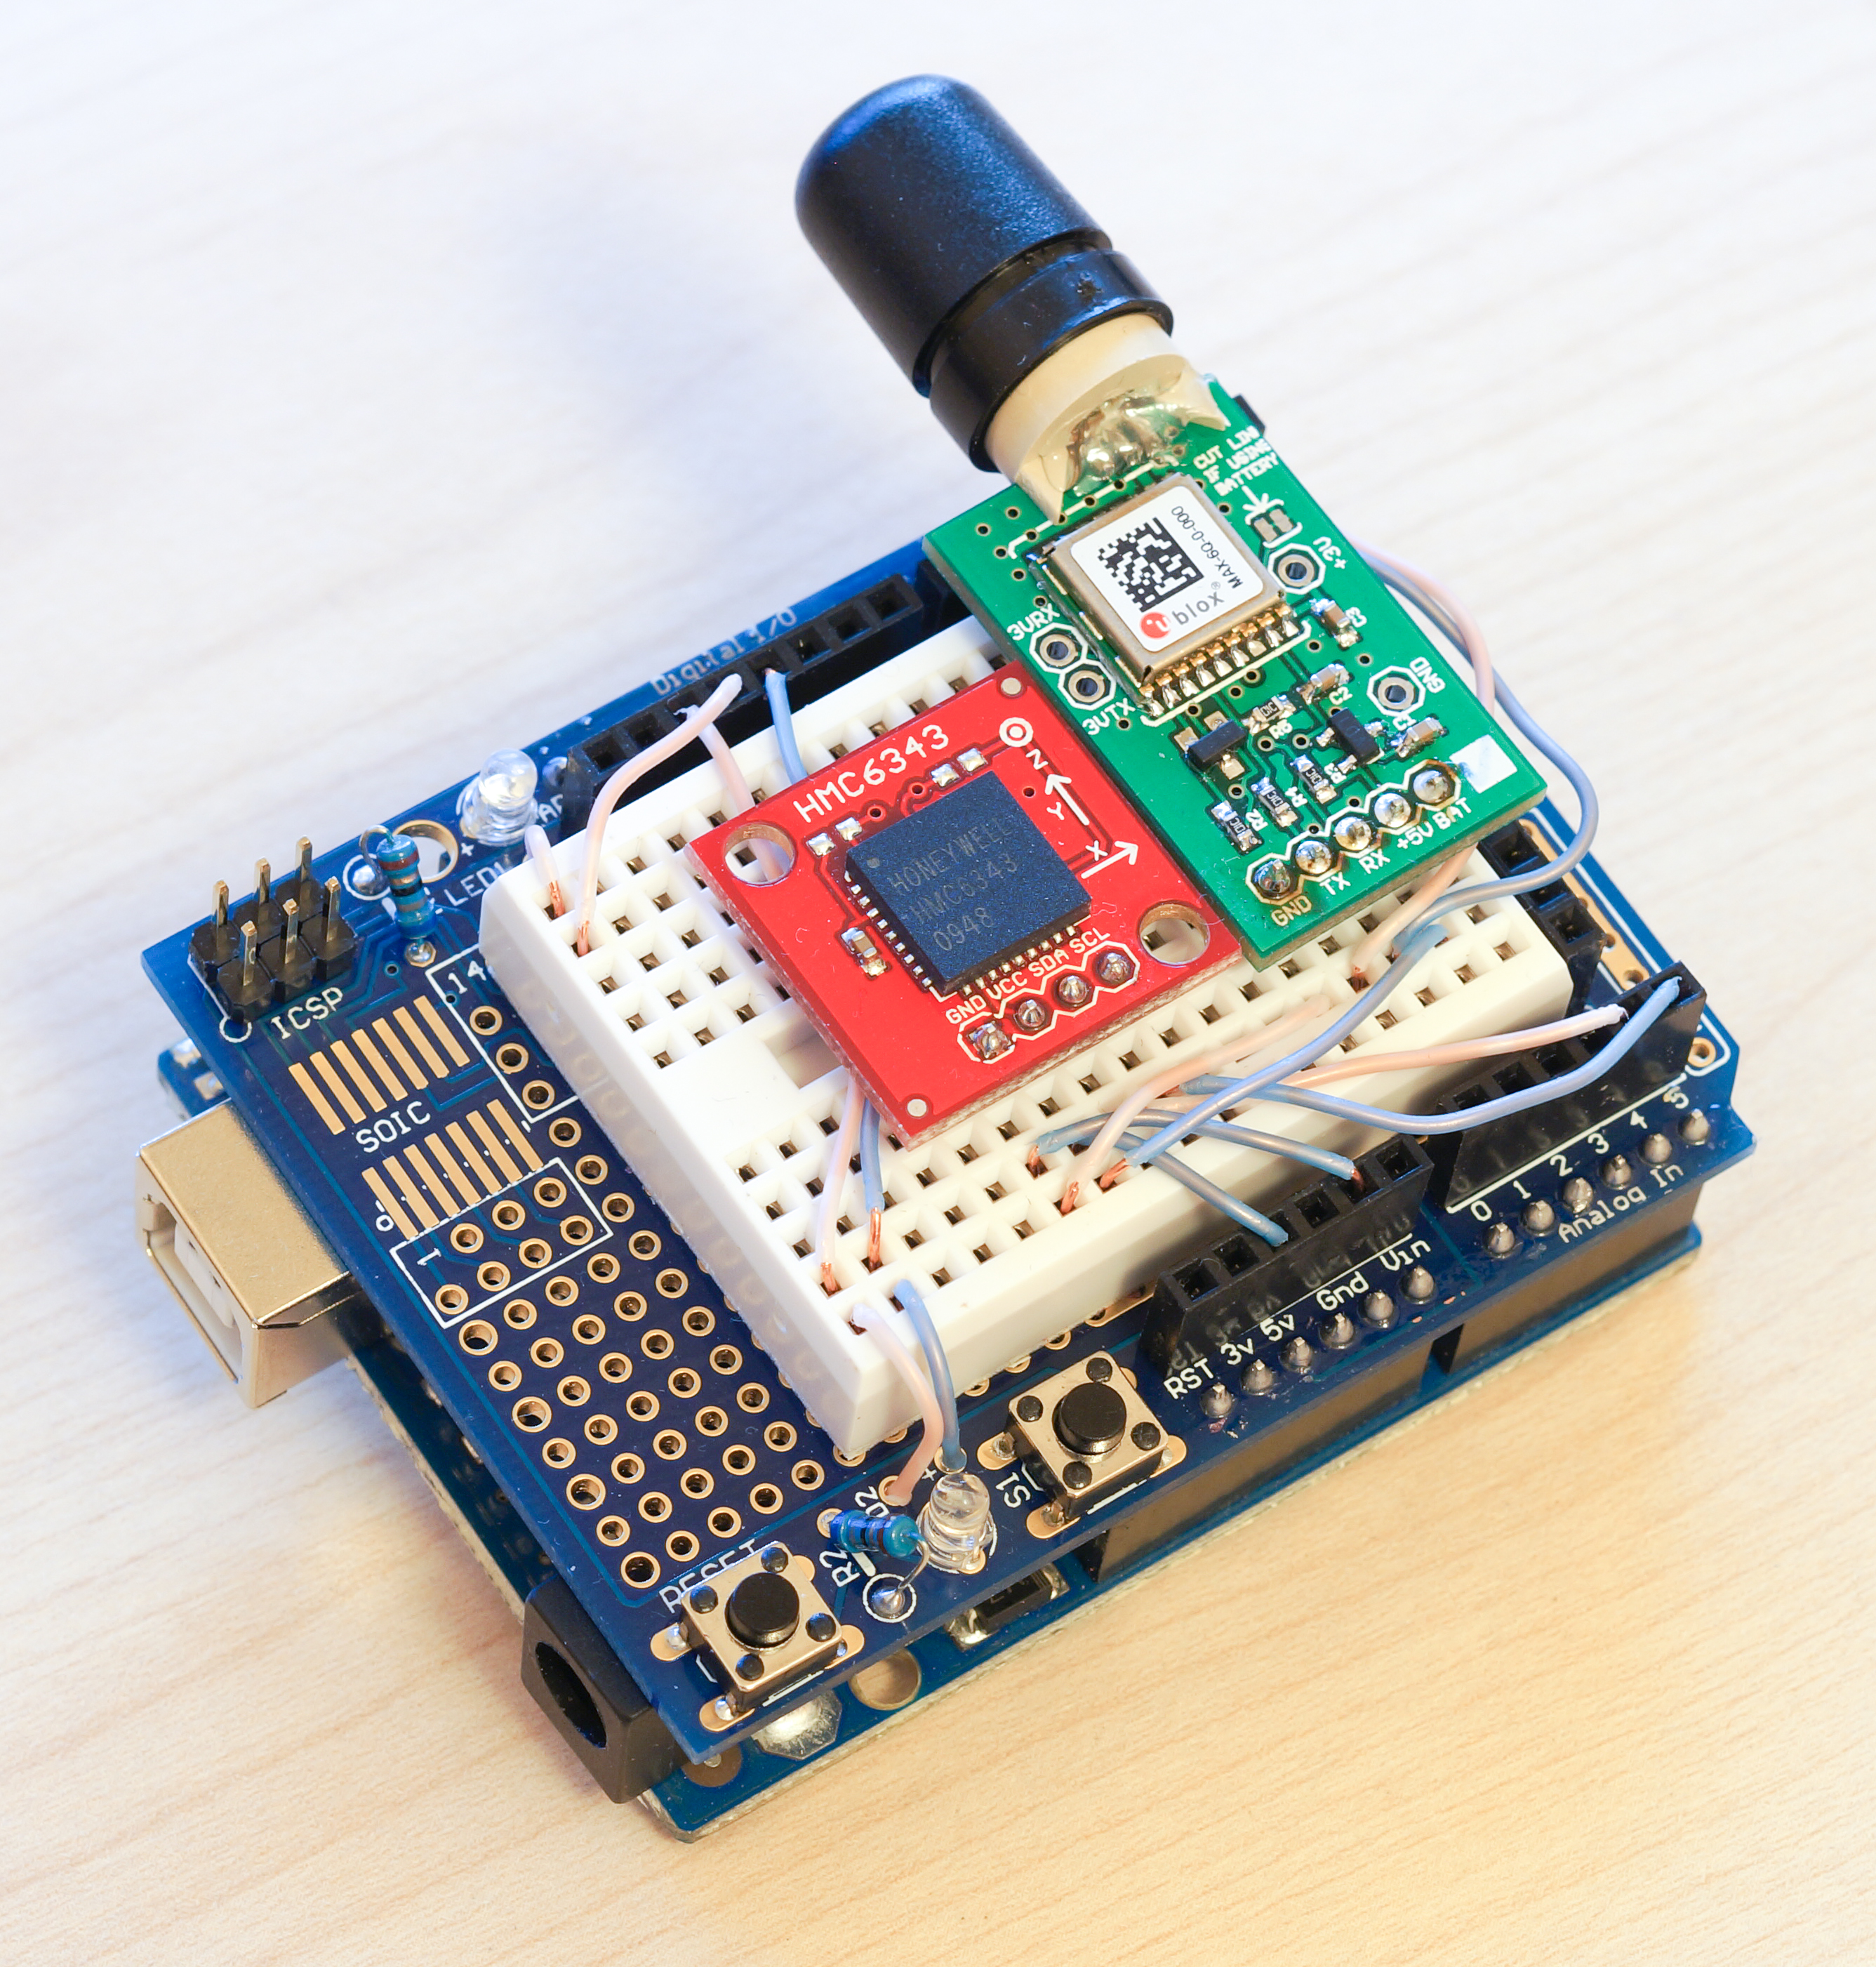
\includegraphics[width=0.48\textwidth]{images/figure_8}
\caption{The HMC6343, MAX-6 and SL-1202 connected via a breadboard prototyping shield to the Arduino, in the setup and configuration that was then attached to the rear of the 110W for the experiments.}
\label{arduino}
\end{figure}

\begin{figure}[h]
\centering
\includegraphics[width=0.48\textwidth]{images/tablet_back}
\caption{The setup from figure \ref{arduino} attached to the rear of the 110W. The sensors are configured such that (in the orientation of this photograph) the X axis is positive pointing straight down, Y is positive pointing straight right and Z is positive pointing perpendicular out of the rear face of the tablet.}
\label{tablet_back}
\end{figure}

Leveraging standard SL avatar/camera control interfaces was explored by programming the Arduino to mimic a standard USB HID joystick via the Lightweight USB Framework for AVRs (LUFA), sending messages that the viewer interpreted as coming from a joystick and allowing the use of the standard joystick options. However the granularity of control attainable via this method was not sufficient and thus the viewer was modified (giving rise to the Pangolin viewer) to make use of the Boost.Asio C++ library to support receiving data via serial port and to use these data to control the movement of the avatar and camera by directly interfacing with the control functions at a lower level of abstraction. Receipt of messages is performed in an asynchronous non-blocking fashion, with the viewer's main loop processing the most recently received message in each iteration. Messages follow the format

$\langle bearing \rangle$ $\langle pitch \rangle$ $\langle roll \rangle$ $\langle latitude \rangle$ $\langle longitude \rangle$

The viewer's GUI was modified with the addition of a dialogue that allows the user to specify the path of the serial device, separately enable or disable sensor-driven camera and movement control, as well as providing numerous controls for fine-tuning its behavior, including the ability to specify high-pass filters for avatar movement and specify the smoothing applied to camera control. This GUI also presents the necessary fields for input of the anchor point details and fields for diagnostic output of the received information. Figure \ref{pangolin_screenshot} shows this GUI within the Pangolin viewer.

\begin{figure}[h]
\centering
\includegraphics[width=0.48\textwidth]{images/figure_9}
\caption{The GUI within the Pangolin viewer that allows administration of the position and orientation control of the avatar. In this screenshot Pangolin is connected to the Arduino and is receiving position and orientation data.}
\label{pangolin_screenshot}
\end{figure}

\section{Results}
Two plausible modalities of interaction were identified for this system, with each presenting different requirements with regards to accuracy of position tracking.

The first modality is one in which a number of locations that represent points of particular interest are identified. This is already a common practice at cultural heritage sites, with such locations often bearing signs or placards presenting text and/or images explaining what can be observed from the position. With Pangolin, when a user walks within a certain range of such a point, their avatar can be moved to the corresponding location within the reconstruction (and a sound played to alert the user to the fact that there is something of interest to observe) from which they can then move the tablet around them to examine their surroundings in the reconstruction. This modality is similar to audio tours employed by many museums and cultural heritage sites, but replaces the requirement to follow a static route or type in numbers of locations with the ability to freely navigate the real environment with access to additional information being triggered automatically once within the required range of a point of interest.

The second modality is one of free roaming exploration, in which the movements of the user's avatar within the reconstruction mimic the user's movements within the real world as closely as possible.
The first modality can be scaled to function with different accuracies of position tracking; as long as the distance between any two points of interest is at least as much as the worst case performance of the position tracking then distinguishing correctly between different points will always succeed. The second modality requires extremely accurate position tracking, arguably surpassing the capabilities of mainstream GPS technology even in ideal situations.

During the experiments the MAX-6 was unable to maintain reception of the additional correction data required for SBAS operation; when left stationary for several minutes reception was possible however subsequent movement of only a few meters at walking pace broke the connection. This reduced the theoretical maximum performance of the unit to 2.5m CEP, with observed performance being lower. Figure \ref{map_one} depicts an aerial view of the St Andrews cathedral ruins; the blue line represents the planned route, red the route recorded by the MAX-6 receiver and green the route recorded by the smartphone for comparative purposes, both while walking the planned route.

\begin{figure}[h]
\centering
\includegraphics[width=0.48\textwidth]{images/figure_4}
\caption{Aerial view oriented North upward of the St Andrews cathedral ruins; the blue line represents the planned route, red the route recorded by the MAX-6 and green the route recorded by the smartphone whilst walking the planned route.}
\label{map_one}
\end{figure}

The Hausdorff distance between the planned route and that recorded by the MAX-6 was $1.02e^{-04\circ}$. The `length' of a degree of latitude and a degree of longitude depends upon location upon the Earth; around the location of the St Andrews cathedral 1$^\circ$ of latitude is equivalent to 111347.95m and 1$^\circ$ of longitude to 61843.88m. Thus the Hausdorff distance of $1.02e^{-04\circ}$ can be visualized as $\pm11.3$m of North/South inaccuracy or $\pm6.3$m of East/West inaccuracy (or a combination of both N/S and E/W inaccuracy not exceeding a total displacement of $1.02e^{-04\circ}$ from the planned route).

The MAX-6 did achieve better performance than the smartphone, which recorded a Hausdorff distance of $1.33e^{-04\circ}$ ($\pm14.8$m N/S, $\pm8.2$m E/W). The Hausdorff distance between the routes logged by the MAX-6 and the smartphone was $1.14e^{-04\circ}$ ($\pm12.7$m N/S, $\pm7.0$m E/W), which represents a low correlation between the inaccuracies recorded by the two receivers even though they are of similar magnitudes from the planned route.

The maximum inaccuracies were recorded when walking along the South wall of the cathedral's nave. This wall is one of the most complete sections of the building with stonework reaching some 30ft above ground level and providing an effective obstruction to line-of-sight to half of the sky (and substantially impairing reception of signals from GPS satellites) when in close proximity to it. When considering just the sub-route shown in figure \ref{map_two}, which terminates before this wall begins to significantly obstruct view of the sky, the Hausdorff distances are notably smaller; the MAX-6 achieved a Hausdorff distance of $7.23e^{-05\circ}$ ($\pm8.05$m N/S, $\pm4.47$m E/W) throughout this sub-route, with the smartphone still behind with $8.99e^{-05\circ}$ ($\pm10.01$m N/S, $\pm5.56$m E/W). Again the Hausforff distance between the receivers showed low correlation between the inaccuracies, at $6.43e^{-05\circ}$ ($\pm7.12$m N/S, $\pm3.98$m E/W).
 
\begin{figure}[h]
\centering
\includegraphics[width=0.48\textwidth]{images/figure_5}
\caption{Aerial view oriented North upward of the St Andrews cathedral ruins; the blue line represents the first sub-route of the planned route, red the sub-route recorded by the MAX-6 and green the sub-route recorded by the smartphone whilst walking the first planned sub-route.}
\label{map_two}
\end{figure}

When analyzing the tracks in the vicinity of the nave (see figure \ref{map_three}) it is shown that although the MAX-6 outperformed the smartphone in terms of Hausdorff distance this relationship can be considered misleading as the smartphone track corresponded more closely in shape to the planned route even if it did stray further at its extreme. The discrepancy in the behavior of the two receivers in this situation is attributed to different implementations of dead-reckoning functionality between the receivers. Dead-reckoning is the process used when a GPS receiver loses reception of location data from satellites and extrapolates its position based upon a combination of the last received position data and the velocity of travel at the time of receiving these data.
 
\begin{figure}[h]
\centering
\includegraphics[width=0.48\textwidth]{images/figure_6}
\caption{Aerial view oriented North upward of the St Andrews cathedral ruins; the blue line represents the second sub-route of the planned route, red the sub-route recorded by the MAX-6 and green the sub-route recorded by the smartphone whilst walking the second planned sub-route.}
\label{map_three}
\end{figure}

Pangolin's camera control from orientation data does not have as stringent performance criteria as the movement control from position data. Unlike augmented reality where sparse virtual content is superimposed upon a view of a real environment and the virtual objects must be placed accurately in order for the effect to work well, cross reality presents a complete virtual environment that is viewed `separately' or side-by-side with the real environment and thus discrepancies between orientation of real and virtual environments have a less detrimental effect to the experience. Although the accuracy of the camera control during the experiments was reported as being sufficient, the speed at which the camera orientation moved to match physical orientation was reported as being too slow, resulting in having to wait for the display to `catch up' to changes in orientation. This is attributed to the 10Hz sampling rate of the orientation sensors which, particularly after readings are combined for smoothing purposes to reduce jerky movement, resulted in too infrequent orientation updates. Frame rates within Pangolin whilst navigating the route averaged between 15 and 20 frames per second with the viewer's `quality and speed' slider set to the `low' position.

The style of explorative interaction with virtual content that this system employs is more resilient to input lag and low frame rates than other scenarios of interaction with virtual content such as fast paced competitive video games including First Person Shooters (FPS) [20], but overall user experience would nonetheless be improved by a faster sampling of orientation data and a higher frame rate. Additionally it should be noted that the cathedral reconstruction was created with relatively powerful desktop computers in mind as the primary deployment platform and has not been optimized for use on less powerful mobile platforms such as Pangolin. Performance of Pangolin on a less graphically complex OpenSim region (Salt Pan 2 [17]), that also depicts a reconstruction of a cultural heritage site, was better at 20 to 25 frames per second at the `low' position and between 15 and 20 frames per second at `high' (see figure 7).

\begin{figure}[h]
\centering
\includegraphics[width=0.48\textwidth]{images/figure_7}
\caption{Plot of Pangolin's performance (measured in frames per second) against different graphical settings (selected via the `Quality and speed' slider of the viewer) in two positions within the Salt Pan 2 region.}
\label{framerate_graph}
\end{figure}

\section{Interpretations}
The positional accuracy of $1.02e^{-04\circ}$ attained by the MAX-6 is sufficient for the first modality of interaction (that of distinguishing and navigating between multiple points of interest). This value of $1.02e^{-04\circ}$ (analogous to a combination of $\pm11.3$m of North/South inaccuracy or $\pm6.3$m of East/West inaccuracy) represents a constraint on the granularity of the content; it is the minimum distance required between any two points of interest for them to be correctly differentiated between. This same value is not sufficient for the second modality of interaction (that of free roaming exploration with avatars mimicking their users' movements as closely as possible). This modality would require the use of additional position tracking techniques to improve accuracy to around 1m CEP (analogous to $8.98e^{-06\circ}$ latitude or $1.62e^{-05\circ}$ longitude around the location of the St Andrews cathedral).

Use of a GPS receiver that is lower performance than the MAX-6 used by Pangolin, but more common due to being of the calibre integrated into smartphones and tablets such as that used in the experiments, is still sufficient for the first modality but with a larger minimum distance required between any two points of interest. The Hausdorff distance of $1.33e^{-04\circ}$ recorded by the smartphone used in the experiments is analogous to $\pm14.8$m N/S or $\pm8.2$m E/W around the location of the cathedral.

Observed accuracy of the orientation tracking is sufficient for both modalities of interaction; the accuracy of orientation tracking required does not change with different positional accuracy and the accuracy of orientation attained in the experiments is sufficient for an acceptable user experience, however the experience would benefit from better graphical quality and higher responsiveness to changes in user orientation.

\section{Conclusions}
Manifestations of PoSR involving 2D content are commonplace, but whilst the social allures and educational benefits of 3D environments have been recognized the ability to forge PoSR situations involving 3D content remains elusive. As development of 3D Web technologies furthers, the demand for 3D PoSR will grow. The cross reality concept, when freed from static linking between physical and virtual environments, provides a technique to address this shortcoming. This technique has been investigated by the Pangolin virtual world viewer as a mobile, location and orientation aware cross reality interface to spatially related 3D virtual environments. Pangolin aimed to provide a platform for furthering previous use of such 3D environments, for allowing students to learn from reconstructions of cultural heritage content, by allowing them to interact with such reconstructions whilst simultaneously exploring the corresponding physical environments.

Performance of position tracking by GPS emerged as a constraint upon the modality of interaction possible in such systems, with commercially available non-assisted GPS receivers, of the quality built into smartphones and tablets, capable of sufficient accuracies for the `points of interest' modality to function correctly but not for the free roaming exploration modality.

These conclusions hold for today's commodity technology. We can expect the resolution, processing power and rendering capability of mobile phones and tablets to continue to increase for any fixed price point. Similarly, augmented positioning systems providing greater positional accuracy are likely to emerge. Thus we conclude that the benefits of having accurate virtual interpretations of historic locations available at the sites in a mobile fashion will be available for school visits, cultural heritage investigation and tourists of the future. As mobile 3D cross reality technology becomes common place and matures, applications in education, entertainment, business and the arts will emerge that will surprise us all.

% ======= ======= ======= ======= ======= ======= =======

\chapter{Mirrorshades}
\graphicspath{ {05_mirrorshades_design_implementation/images/} }
\begin{quote}
	\textit{``A vacant-eyed clerk glanced up at me \ldots\ He was wearing a bifocal visor, which gave him a semitransparent view of the OASIS while also allowing him to see his real-world surroundings.''}%~\cite{Cline2012}
\end{quote}
\hfill \textit{Ready Player One, Ernest Cline}
\\
\\

%=========================================================================================================

\label{chapter-mirrorshades}

This chapter discusses the design and development of a parallel reality platform that combines a wide field of view (FOV), stereoscopic 3D, VR head mounted display (HMD) modified with cameras, with an indoor positioning system (IPS), allowing its user to observe and move around their real environment imbued with the ability to alternatively view an immersive VR environment from the equivalent vantage point. Creation of this platform addressed the shortcomings identified in the VTW platform, by using more accurate position tracking, faster and more responsive orientation tracking and a more immersive virtual display.

%Previous XR research approached the vacancy problem by integrating sensor/actuator networks into the environments, such that actions in one could manifest in the other, however direct visual engagement with the virtual environment was only possible from static interfaces at pre-determined locations within the real environment~\cite{Lifton2007a, Dublon2011}. The platform discussed in this document addresses this shortcoming by providing a mobile interface for visual engagement with both environments of a XR system, allowing the user to transition between viewing their real environment and a virtual environment at any time while maintaining the freedom to move around them, multiplexing visual stimuli from their real surroundings and from a parallel, virtual `mirror world'~\cite{Gelernter1993}.

%=========================================================================================================

%A second example of such a situation is found in the book \textit{Ready Player One}, in a scene in which the protagonist users the equivalent of an Internet cafe to access the \textit{OASIS};

%The OASIS is similar to Snow Crash's Metaverse; a fictional multi-user 3D environment with no enforced likeness to the real world, accessed via \textit{``a visor and a pair of haptic gloves''}. The bifocal visor allows this character to switch his attention between the virtual environment of the OASIS and his real surroundings in the Internet cafe.

%=========================================================================================================

\section{Learning from VTW}
The development of the VTW platform as a first foray into applying the concept of PR to the field of virtual heritage revealed reservations around quantitative performance and qualitative experience. Firstly and most critically, the accuracy of position tracking attainable by using a GPS receiver, even one of higher specification and real world performance than those commonly found in smartphones, was not sufficient for the envisaged style of interaction. Secondly, the ability of a hand held  display (the tablet) to provide immersive 3D graphics of a complete, atmospheric reconstruction was limited. Moving forward from VTW, a new project was embarked upon to address these concerns with aims to greatly improve the experience of PR in a virtual heritage scenario.

In contrast to VTW, which was intended for outdoor use upon cultural heritage sites where either no remnants or only parts of original structures still stand, the successive platform was intended for use indoors. This not only allowed the investigation of the application of PR to cultural heritage to be expanded to indoor scenarios, for sites where more of a historic structure still stands, but also allowed for the use of an IPS, many of which offer substantially more accurate proven real world accuracy than GPS does for outdoor positioning.

Furthermore, in place of a hand held display such as the tablet used by VTW, the successive platform makes use of a head mounted display offering stereoscopic 3D graphics over a wide field of view, that promises much greater immersion, with a head tracking solution that substantially outperforms the orientation tracking employed by VTW both in terms of accuracy and responsiveness.

%=========================================================================================================

\subsection{The Mirrorshades Platform}

Figure \ref{systemarchitecture} presents a high level architectural overview of the successive PR platform, dubbed Mirrorshades\footnote{\textbf{Mirrorshades: The Cyberpunk Anthology} (1986) is a defining cyberpunk short story collection edited by Bruce Sterling, who explains how mirrored sunglasses became a literary badge or totem for the cyberpunk movement, whose fiction has frequently involved immersive multi-user virtual environments and head mounted displays.}. This is a parallel reality platform which allows its user to observe and move around their RW environment whilst wearing a HMD, with their position tracked by an IPS, switching between viewing RW visual stimuli provided by cameras mounted to the HMD and VR visual stimuli from the equivalent vantage point of the reconstruction, as tracked by the IPS. A controller held by the user allows them to trigger these switches between RW and VR. The mobile client that produces the graphical content delivered to the HMD can is carried about the person in a bag/satchel.

\begin{figure}[h]
	\begin{center}
		\includegraphics[width=.5\linewidth]{system-architecture.png}
		\caption{High level overview of the Mirrorshades parallel reality platform.}
		\label{systemarchitecture}
	\end{center}
\end{figure}

Emphasis should be placed on the fact that the two views, RW and VR, through the function of IPS and head tracking combined with the spatial equivalence of the constituent environments, represent equivalent vantage points within the two environments, differentiating the modality of interaction from the visual perception exchange systems exhibited in an Istanbul church by Mathieu Briand;

\begin{quote}
	\textit{``In an earlier version, set in the Hagia Eirene church in Istanbul, visitors wearing a wireless headgear viewing device could press a button to exchange the image on the screen with that of another of the six headgear cameras, revealing whatever it was pointing at. Visitors were fascinated by the dynamic visual transformations, such as the way the brightly painted floor could suddenly be replaced by the church dome as they wandered around the space.''}~\cite{Jones2006}
\end{quote}

Likewise, the modality of interaction provided by the Mirrorshades platform distances itself from that of Briand's later experiments into `controlled schizophrenia', in which displacement of body and visions were intentional;

\begin{quote}
	\textit{``The audience members wear helmets that incorporate a camera, goggle-style compact monitor, and headphones. The audience members may also carry a connector that can be plugged and unplugged from the nine sockets placed around the museum, in order to exchange audiovisual experiences with others.}

	\textit{When a connector is not plugged into a socket, one sees the environment through his/her own camera. In other words, one walks around seeing the surrounding environment through his goggle monitor. When the connector is plugged into a socket on the wall, the person sees the view taken by one of the three cameras installed in the building, or taken by another camera worn by another audience member whose camera is also connected to a socket.''}~\cite{Jones2006}
\end{quote}

As the different views that a user of the Mirrorshades platform switches between are inherently the same `place', seen from the same vantage point.

%=========================================================================================================

\subsection{St Salvator's Chapel}

The stage upon which the Mirrorshades platform was designed and developed to perform upon was St Salvator's chapel in St Andrews. Founded in 1450 but internally stripped of its medieval fittings during the Protestant Reformation (1517 - 1648), the chapel looks markedly different in the present day than it did upon its completion. An existing VR reconstruction of the chapel as it stood in the period 1450-1460 and the marked differences between the internal appearance of the VR building and the current building (including the replacement of the original stone roof with a wooden one and drastically different dividing of the internal space) make this chapel an ideal candidate within the context of cultural heritage for the Mirrorshades PR system to be deployed. The magnitude of the changes between the chapel's original state and how it stands today means that AR would not in fact be able to present a faithful image of how the chapel originally looked, but would need to be combined with substantial application of diminished reality to remove present day features that were not there in the past.

\TwoFig{sallies-vrst/sallies-quad-real.jpg}{St Salvator's chapel today.}{sallies-quad-real.jpg}
       {sallies-vrst/sallies-quad-virtual.png}{St Salvator's chapel reconstruction.}{sallies-quad-virtual.png}
       
This reconstruction project has virtually recreated St Salvator’s chapel as it was built and furnished for Bishop James Kennedy between 1450 and 1460. The chapel was of the greatest significance for the new architectural ideas that it introduced into Scotland, at a time when Scotland was particularly open to external artistic influences. However, although the shell of the chapel survives and remains in use, it has lost its vault, its window tracery and its liturgical furnishings, and it now requires specialist skills to appreciate the quality of its original state. As with other reconstructions from the OVW group, the virtual St Salvator's chapel is a product of a collaboration between architectural, art history and computer science scholarship. On the combined evidence of a highly detailed late medieval inventory and of the architecture itself, it has been possible to show how the chapel was furnished internally with altars, choir stalls, lecterns, screens, stained glass and wall paintings and the virtual chapel is enhanced with lighting. The architectural, liturgical and spatial analysis allows our understanding of the history of the Chapel as a living building to be enormously enhanced by experiencing the building in its original context.

\TwoFig{sallies-vrst/sallies-real-toward-altar.jpg}{St Salvator's chapel looking East, present day.}{sallies-real-toward-altar.jpg}
       {sallies-vrst/sallies-virtual-toward-altar.png}{St Salvator's chapel looking East, reconstruction.}{sallies-virtual-toward-altar.png}

The chapel is an aisle-less rectangle with a three-sided east apse. Deeply projecting three-stage buttresses define the bays, which are now capped by pinnacles of 1861-2. The windows which occupy the full space available between the buttresses no longer reflect their original forms. The main entrance to the chapel was through a doorway in the second bay from the west of the south flank, which is covered by a vaulted porch between the buttresses. Two doorways on the north side presumably opened into a lost sacristy and treasury range.

The interior of the chapel is known to have been covered by a stone vault, which is assumed to have been of pointed barrel form with a decorative pattern of ribs, like the small vault over the south porch. The interior is now covered by an inappropriate timber roof.

\TwoFig{sallies-vrst/sallies-real-from-altar.jpg}{St Salvator's chapel looking West, present day.}{sallies-real-from-altar.jpg}
       {sallies-vrst/sallies-virtual-from-altar.png}{St Salvator's chapel looking West, reconstruction.}{sallies-virtual-from-altar.png}

St Salvator’s chapel is considered the first Scottish example of a church planned with an aisle-less rectangular main body terminating in a polygonal eastern apse, a type that was to have a long future for a range of Scottish church types. Such chapels were common in university colleges in France and since Bishop Kennedy had a highly placed kinsman in the university of Paris and drew many ideas for the organisation of his college from that university’s constitution, it is reasonable to assume that he also drew some of his ideas for the architecture of his chapel from there. On this basis, St Salvator’s must be seen as an outstandingly important channel for the introduction into Scotland of new architectural ideas from France. The new architecture made a significant statement in its Scottish context. 

The reconstruction of the chapel involved both the mental reconstruction of modified and lost features, and the establishment of the range of ways in which buildings that represent a spirituality alien to modern students were intended to function. As such it offers an invaluable academic discipline for those involved in the reconstruction, providing eminently practical ways of testing theories and assumptions. It is then of the greatest value for conveying more widely the understanding that has been gained. The development of a PR system which enables comparison between the real and virtual chapel in the same time and place aims to further enhance the value of the reconstruction.

%=========================================================================================================

\section{Virtual Reality Head Mounted Displays}
The concept of virtual reality and the associated head mounted displays that provide wide field of view, stereoscopic 3D graphics coupled with head tracking is currently experiencing a resurgence of interest and investment, thanks largely to the advent of Oculus and their Rift platform. Whilst the first head mounted computer display was created in the late 1960s by Ivan Sutherland~\cite{Rheingold1992}, it was not until the late 1980s and early 1990s that VR began to be pushed to the consumer. Unfortunately, both the hardware and software was not ready for consumer adoption at this time and these systems failed to live up to the substantial hype of being a \textit{``revolutionary technology''} which \textit{``promises to transform society''} (figure \ref{rheingold-virtual-reality.jpg}), resulting in the VR bubble bursting.

\begin{figure}[h]
	\begin{center}
		\includegraphics[width=0.4\textwidth]{rheingold-virtual-reality.jpg}
		\caption{Howard Rheingold's 1992 bestseller \textit{Virtual Reality}~\cite{Rheingold1992}.}
		\label{rheingold-virtual-reality.jpg}
	\end{center}
\end{figure}

Decades after this initial disappointment with consumer VR, Oculus now looks set to finally begin realising a successful consumer VR platform, thanks largely to the substantial advances in display technologies made during the past decade driven by the explosive popularity of smartphones and tablets. Pre-Oculus HMDs predominantly made use of two separate microdisplays, one for each eye; Sutherland's original `Sword of Damocles' made use of two tiny CRT screens, whilst later HMDs made use of two OLED microdisplays. As the number of market applications for microdisplay technology was (\& continues to be) relatively small, there are limited models to chose from and they command high prices when considering integration into a consumer device.

Oculus have taken a different approach for their Rift HMD. Instead of using two small displays, one for each eye, it uses a single larger display upon which two separate images are rendered, side-by-side. This approach has two distinct advantages compared to prior dual display techniques. Firstly, the complexity of the device is reduced, which effects both price, integration and content development. Secondly, the cost of a single display in the 5"-7" range is drastically lower than the cost of a pair of microdisplays, thanks to the surging popularity of smartphones and tablet computers. By making use of readily available displays intended for smartphone/tablet manufacturers, Oculus were able to bring their first Development Kit (DK1) to market for researchers and enthusiasts at a price of only \$300, but still providing substantially wider FOV than the vast majority of existing HMDs (even those with vastly higher price points).

For comparison, examples of consumer-grade commercial HMDs that use the twin OLED microdisplay approach, the Sony HMZ-T1, which launched with a price of \textyen60,000 (\$800 at exchange rates of the time) and its successor the HMZ-T2 which launched with a price of \textyen70,000 (\$900 at exchange rates of the time), provide $45\textdegree$ horizontal FOV/$51.6\textdegree$ diagonal and no head tracking (intended primarily as a personal 3D cinema experience), whilst Oculus' DK1 provides more than $90\textdegree$ horizontal and $110\textdegree$ diagonal FOV. Furthermore, the DK1 integrates a head tracking solution operating at a rate of 1kHz and providing best in class accuracy. Combined with advances in both hardware and software tasked with producing 3D graphics, the user experience of Oculus' HMD offerings is promising to finally deliver on the VR promises of 30 years previous.

The March 2014 acquisition of Oculus by Facebook\footnote{\url{https://www.facebook.com/zuck/posts/10101319050523971}} for \$2 billion\footnote{\url{http://www.theguardian.com/technology/2014/jul/22/facebook-oculus-rift-acquisition-virtual-reality}} and Oculus partnership with Samsung, one of the world's leading display manufacturers, which has already led to the release of an innovative VR HMD that makes use of an existing smartphone as its display\footnote{\url{https://www.oculus.com/gear-vr/}}, lends hope that this wave of VR hype will succeed where its hype-laden 90's cousin failed.

%\textbf{***Maybe talk about what other HMDs there were actually available to me on the market? Vuzix 1200/900/whatever?}

%take bits from that youtube video from Samsung developers?

%=========================================================================================================

\subsection{The Oculus Rift DK1 and Unity Game Engine}

The OVW group took delivery of an Oculus Rift DK1 from the first batch of units shipped to the EU, in August 2013. The immersive experience of using the DK1, thanks to its wide FOV, fast and accurate head tracking, stereoscopic 3D and novelty compared to traditional 2D displays, easily met the requirements of the display aspect of the Mirrorshades platform to exceed that of VTW in terms of user experience.

At this early stage in the DK1's release, the best supported software platform in terms of API provision and integration was the Unity game engine. After experience with modifying the Second Life client with the VTW project, it was decided prudent to convert the OVW group's OpenSim model of St Salvator's chapel into a Unity compatible format, rather than embarking upon further modification to the Second Life client to support the DK1.

One deciding factor in this deliberation was the more stringent performance requirements for an enjoyable HMD experience compared to those of a traditional desktop/handhend display experience; when using a HMD such as the DK1, a high and smooth framerate is required to avoid a kind of motion sickness referred to as `simulator sickness', with Oculus' official guidelines being for Rift applications to \textit{``run at a frame rate equal to or greater than the Rift display refresh rate''}\footnote{\url{http://static.oculus.com/sdk-downloads/documents/Oculus_Best_Practices_Guide.pdf}} which in the case of the DK1 is 60Hz. Due to the possibly ephemeral nature of Second Life content, where users are free to create, modify and destroy content in real time, Second Life as a 3D platform suffers in terms of performance compared to game engines such as Unity due to not being able to exploit techniques such as occlusion culling~\cite{willmott:largecomplex} as these require an offline processing phase that depends upon environmental content to be static and unchanging. The OVW group's experience in presenting Second Life/OpenSim content on a range of different hardware did not point to good odds of managing to render the St Salvator's chapel scene at 60fps, especially when considering that stereoscopic rendering introduces an overhead even when the total resolution of the two side-by-side images is no greater than the single monoscopic image. As Mirrorshades is a mobile application and the computer producing the visuals is carried by the user, the specification of this client are also limited compared to those that the group has used in alternative static deployments.

\textbf{***Some fps graphs of Second Life vs Unity in chapel with Clevo?}

%=========================================================================================================

\subsection{Modifying the DK1 for See Through Video}
\label{modifying-dk1}
The Oculus Rift DK1 covers the user's entire view, such that they cannot see any of their real world surroundings whilst wearing it, and it does not feature any camera provision to allow a mediated view of the real world to be presented to the user. As such, it was necessary to modify the DK1 to provide such capability. When choosing cameras for this task, there were several desired ideal features;
\begin{itemize}
	\item resolution and refresh rate that match (or exceed) those of the DK1,
	\item sensor aspect ratio that matches that of the DK1's display halves,
	\item combined lens focal length and sensor dimension to provide wide FOV (ideally matching the FOV of the DK1),
	\item ease of integration with the Unity platform.
\end{itemize}

The PS3 Eye camera met most of these requirements. It's resolution is only 640x480 pixels, whilst each half of the DK1's display is 640x800 pixels, however unusually for a USB camera it is capable of running at 60fps (the refresh rate of the DK1). The aspect ratio of the 640x480 sensor is 4:3, which although not identical to the 5:4 aspect ratio of each eye's 640x800 `half' of the DK1 screen is closer than the 16:10 or 16:9 aspect ratio of a `widescreen' camera sensor. Furthermore, once dismantled to its bare PCB it features mounting holes for a standard S-mount (M12x0.5mm) lens mount commonly used for CCTV cameras, allowing alternative focal length lenses to be easily fitted.

A very early test with the PS3 Eye and the DK1\footnote{\url{https://www.youtube.com/watch?v=tS0FGZxQzCU}} was performed by simply attaching a single unmodified PS3 Eye camera to the top of the DK1 (figure \ref{rift-pseye-ziptied.jpg}), with its stock lens set to its `wide' setting (75\textdegree, presumably diagonal, FOV\footnote{\url{http://uk.playstation.com/media/247868/7010571 PS3 Eye Web_GB.pdf}}). One purpose of this test was to explore the suitability of Unity's \texttt{WebCamTexture}\footnote{\url{http://docs.unity3d.com/ScriptReference/WebCamTexture.html}} feature for integrating the stream from a USB camera into a 3D application. In this early test, the mediated RW video stream was rendered to a small `floating' window that moved with the user's head (figure \ref{floating-webcam-window.png}), allowing the user to view both environments at once, with the real environment in their peripheral whilst they were attending to the virtual. Whilst an interesting concept, the decision was made to instead render the mediated RW stream to the full DK1 screen so as to allow the user to better observe their real environment thanks to the larger image and higher resolution, with the small floating window likened more to the VTW approach of PR than an experience that allows true immersion in the environment of choice. A second benefit of this switching approach is that it helps to mitigate any detrimental affect of latency in the camera image(s) not matching that of the virtual image(s).

\TwoFig{rift-pseye-ziptied.jpg}{Oculus Rift DK1 with PS3 Eye test.}{rift-pseye-ziptied.jpg}
       {floating-webcam-window.png}{`Floating' window see through video in Unity.}{floating-webcam-window.png}

A pair of PS3 Eye cameras were dismantled, removing their outer plastic housing and stock lenses then fitting S-mount lens mounts. Ideally, the lenses used would provide the same FOV as the Rift itself is capable of displaying, such that the mediate RW stream from the cameras could be displayed at the full size of the Rift and `match' the FOV of whatever virtual content would alternatively be displayed. However there is a trade off with lenses between focal length and distortion; shorter focal lengths mean a wider FOV, however they also introduce more distortion which is not necessarily corrected by the shader that the Rift uses to compensate for the distortion of its own plastic lenses through which the image is viewed.

The PS3 Eye has a `1/4'' type' sensor which is only an indication of its true dimensions\footnote{\url{http://www.dpreview.com/glossary/camera-system/sensor-sizes}} and as Sony has not published the actual dimensions of the sensor we adopt the typical 1/4'' type dimensions\footnote{\url{http://www.photoreview.com.au/tips/buying/unravelling-sensor-sizes}} of 4.5mm diagonal, 3.6mm horizontal, 2.7mm vertical for calculating FOV estimations. Empirical accounts of very short focal length S-mount lenses mounted to the PS3 Eye camera indicated that the distortion becomes very high beneath 2.1mm\footnote{\url{http://peauproductions.com/store/index.php?main_page=index&cPath=26_4}}. Table \ref{fov-table} gives the diagonal, horizontal and vertical FOV of the widest readily available S-mount lenses. Whilst 1.7mm lenses would provide almost identical FOV to the Rift's display (105.9\textdegree\ diagonal for the cameras, 110\textdegree\ diagonal for the Rift) the amount of distortion introduced would likely be of such an extent that the experience of viewing the mediate RW environment would be degraded more by distortion than by limited/non-matching FOV of longer focal length lenses, unless the lens' distortion was compensated in a separate stage.

\begin{table}
\begin{center}
\begin{tabularx}{\textwidth}{c *{4}{>{\centering\arraybackslash}X}}
\toprule
\textbf{Focal length (mm)} & \textbf{Diagonal FOV (\textdegree)} & \textbf{Horizontal FOV (\textdegree)} & \textbf{Vertical FOV (\textdegree)} \\
\midrule
2.5mm & 84    & 71.5 & 56.7 \\
2.1mm & 93.9  & 81.2 & 65.5 \\
2.0mm & 96.7  & 84   & 68 \\
1.9mm & 99.6  & 86.9 & 70.8 \\
1.8mm & 102.7 & 90   & 73.7 \\
1.7mm & 105.9 & 93.3 & 76.9 \\

\bottomrule

\end{tabularx}
\caption{FOV of various focal length lenses resolving onto a 1/4'' type sensor.}
\label{fov-table}
\end{center}
\end{table}

However, using a lens with a short enough focal length to provide a FOV as wide as the Rift isn't strictly necessary as, when wearing the Rift, the edges of the image presented to each eye are not necessarily visible to the user, especially if the Rift's adjustable distance from the eyes is adjusted such that it sits at its furthest position. Such adjustment is actually prudent for a user study, as using the Rift at its maximum extension from the eyes ensures maximum compatibility and comfort with users and also removes a variable between users compared to if each user is permitted to chose the extension themselves. Thus the choice of lens can be dictated by identifying the FOV required to fill the portion of the Rift's images that are visible when the headset is extended to its maximal position, rather than by matching the Rift's overall FOV, possibly allowing the use of lenses with focal length long enough that the distortion they introduce is not so bad as to require a separate correction phase.

Experiments revealed that with the DK1 set to its maximum extension, the area of the images visible to the user was wider than that provided by 2.5mm lenses (84\textdegree\ diagonal) when scaled correctly and narrower than that provided by 2.1mm lenses (93.9\textdegree\ diagonal) when scaled correctly. Without easy availability of a lens with a focal length between 2.5mm and 2.1mm it was decided to make use of the 2.1mm lenses. Figure \ref{lens-comparison-on-ps3eye-pcb.jpg} shows the 2.5mm lens (right) and 2.1mm lens (left) mounted to the PS3 Eye PCBs via S-mount lens mounts, while figure \ref{fov-comparison-1.png} shows the FOV of the selected 2.1mm lenses scaled correctly upon the wider FOV of the DK1's images - as previously mentioned, with the DK1 at its furthest extension, users cannot perceive the area outwith the mediated camera image.

\TwoFig{rift-clips-cameras/lens-comparison-on-ps3eye-pcb.jpg}{S-mount lenses on PS3 Eye camera PCBs.}{lens-comparison-on-ps3eye-pcb.jpg}
       {fov-comparison-1.png}{FOV comparison between DK1 and 2.1mm lenses.}{fov-comparison-1.png}

%{fov-comparison-2.png}{}{fov-comparison-2.png}

The PS3 Eye cameras were mounted to the DK1 by modifying the 3D printable sensor mount design released by the University of Southern California Institute for Creative Technologies\footnote{\url{http://projects.ict.usc.edu/mxr/diy/oculus-sensor-mount/}}. The modified mount comprised a base piece (figure \ref{clips.jpg}) that clips securely over the front of the DK1 and a slotted plate (figure \ref{clips-hori-plate.jpg}) onto which the PS3 Eye cameras are mounted. These parts were 3D printed using a MakerBot Replicator 2X\footnote{\url{http://store.makerbot.com/replicator2x}} and then combined using epoxy resin. The combination is shown attached to the DK1 by figure \ref{hori-1.jpg}. The slots in the slotted plate are spaced to match the mounting holes of the PS3 Eye PCB, such that the cameras can be attached by metal stand-offs (figure \ref{hori-2.jpg}) and can then be easily moved left and right to alter the distance between them to account for different interpupillary distances. Figure \ref{hori-3.jpg} shows how one camera is mounted upside down to allow enough clearance for the PCBs to be moved close enough together to accommodate short interpuillary distances.

\begin{figure}[h]
    \centering
    \begin{minipage}{.32\textwidth}
        \centering
        \includegraphics[width=\textwidth]{rift-clips-cameras/clips.jpg}
        \caption{Camera mount base.}
        \label{clips.jpg}
    \end{minipage}%
    \hspace{.01\textwidth}
    \begin{minipage}{0.32\textwidth}
        \centering
        \includegraphics[width=\textwidth]{rift-clips-cameras/clips-hori-plate.jpg}
        \caption{Camera mount slotted plate.}
        \label{clips-hori-plate.jpg}
    \end{minipage}%
    \hspace{.01\textwidth}
    \begin{minipage}{0.32\textwidth}
        \centering
        \includegraphics[width=\textwidth]{rift-clips-cameras/hori-1.jpg}
        \caption{Camera mount attached to DK1.}
        \label{hori-1.jpg}
    \end{minipage}
\end{figure}

\TwoFig{rift-clips-cameras/hori-2.jpg}{Cameras mounted using stand-offs.}{hori-2.jpg}
       {rift-clips-cameras/hori-3.jpg}{Two PS3 Eye cameras mounted on DK1.}{hori-3.jpg}

Although the initial integration test with a single PS3 Eye camera revealed easy accessibility of the camera within Unity, using two PS3 Eye cameras proved temperamental. Unity's \texttt{WebCamTexture} support identifies webcams via their `name' as provided by their driver. In the case of the PS3 Eye using the driver provided by Code Laboratories\footnote{\url{https://codelaboratories.com/products/eye/driver/}} (this third party driver must be used as no official Windows driver is available with Sony only marketing the PS3 Eye for use with their PS3 console) an issue arises where both cameras present the same name to Unity and the second camera overwrites the reference to the first, only allowing access to a single camera. Figure \ref{ps3-eye-unity-overwrite.png} shows this issue, that whilst Windows' device manager successfully identifies both cameras independently, Unity's \path{WebCamTexture.devices()} function returns a reference to only one (the \texttt{BisonCam, NB Pro} entry is the laptop's internal webcam). A partial solution to this issue was presented by a community provided Unity package\footnote{\url{http://tips.hecomi.com/entry/20130731/1375279561} (Japanese)}, which allowed the setup up to be successfully tested within a departmental building\footnote{\url{https://www.youtube.com/watch?v=oy5NqqDtkJ4}}.

\begin{figure}[h]
	\begin{center}
		\includegraphics[width=.8\linewidth]{ps3-eye-unity-overwrite.png}
		\caption{Unity failing to instantiate references to multiple PS3 Eye cameras.}
		\label{ps3-eye-unity-overwrite.png}
	\end{center}
\end{figure}

An oversight in the design of the camera mounts was realised by when William Steptoe later released details of his `AR Rift' project\footnote{\url{http://willsteptoe.com/post/66968953089/ar-rift-part-1}}. Although the DK1's overall screen has a resolution of 1280x800 in a `horizontal' 16:10 aspect ratio, each `half' of this screen as presented individually to each eye has a resolution of 640x800 in a `vertical' 4:5 aspect ratio. Thus to best match the aspect ratio of a 4:3 camera sensor, such as that of the PS3 Eye, to each half of the DK1's screen, that camera should be oriented in a portrait orientation rather than the landscape orientation employed thus far by the Mirrorshades platform with the PS3 Eye cameras. Thus new mounting hardware was designed and printed, by further modification of the USC's original 3D designs, allowing for vertical mounting of the PS3 Eye cameras. This new design is shown in figure \ref{clips-vert.jpg} (the recessed section in the centre of the clip allows for the heads of bolts to clear the front of the DK1) and the assembled units are shown attached to the DK1 in figure \ref{vert-6.jpg}. Additionally soon after this point, the metal stand-offs that had been used to mount the camera PCBs to the clips (see figure \ref{vert-1.jpg}) were replaced with a combination of rubber washers and threaded bolts (see figure \ref{vert-4.jpg}) both to reduce the discrepancy in the mediated RW images caused by the distance between the camera sensors and the user's eyes (by reducing this distance) and to allow for finer alteration of the orientation of the cameras.

\TwoFig{rift-clips-cameras/clips-vert.jpg}{Updated camera mount.}{clips-vert.jpg}
       {rift-clips-cameras/vert-6.jpg}{PS3 Eye cameras using updated mounts.}{vert-6.jpg}

\TwoFig{rift-clips-cameras/vert-1.jpg}{Updated camera mount with stand-offs.}{vert-1.jpg}
       {rift-clips-cameras/vert-4.jpg}{Updated camera mount with rubber washers.}{vert-4.jpg}

Unfortunately the PS3 Eye naming solution was temperamental at best and two camera compatibility was frequently lost. It was decided prudent to therefore replace the PS3 Eye cameras with alternatives, rather than attempting to glean a solution to their reliable compatibility with Unity. Using Steptoe's project as a guide, a pair of Logitech C310\footnote{\url{http://www.logitech.com/en-gb/product/hd-webcam-c310}} cameras were sourced. Whilst the stated refresh rate of the C310 is only 30Hz, half that of the PS3 Eye, it supports a resolution of 1280x960, which is higher than that of the PS3 Eye and of each half of the DK1's display. Thus the switch from the PS3 Eye cameras to the C310 represented a sacrifice in framerate, but an increase in resolution. Empirically the increase in resolution was however indiscernible, likely due to the effect of the DK1's optics reducing the visual acuity of its display, whilst the reduction in framerate was more prominently noticeable.

The C310 cameras received the same attention as the PS3 Eye cameras; they were dismantled and outfitted with S-mount lens mounts. As the sensor in the C310 is also of the 1/4" type, the FOV provided by the 2.1mm lenses on the C310 cameras is comparable to that of the same lenses mounted to the PS3 Eye cameras. Due to the lack of mounting holes present on the C310 PCB, the PCBs were set into a thin sheet of thermoplastic (figure \ref{thermoplastic.jpg}) which was then attached to the 3D printed clips with the same rubber washer and threaded bolt arrangement as the PS3 Eye cameras. The assembled DK1 + dual C310 solution is shown by figures \ref{vert-7.jpg} (3/4 view), \ref{middle.jpg} (profile view) and \ref{right.jpg} (detail view).

\TwoFig{rift-clips-cameras/thermoplastic.jpg}{Setting C310 PCBs into thermoplastic.}{thermoplastic.jpg}
       {rift-clips-cameras/vert-7.jpg}{C310 mounted to DK1 (three-quarter view).}{vert-7.jpg}

\TwoFig{rift-clips-cameras/middle.jpg}{C310 mounted to DK1 (front view).}{middle.jpg}
       {rift-clips-cameras/right.jpg}{C310 mounted to DK1 (detail view).}{right.jpg}

%=========================================================================================================

\subsection{Switchable Stereoscopic See Through Video with Unity}

Unity's \texttt{WebCamTexture} support was used to gain access to the C310 video streams within Unity. Due to better provisioned drivers, there was no issue with Unity obtaining references to both C310 as there had been with two PS3 Eye cameras. These video streams were applied to a pair of planes, of matching orientation and aspect ratio to the video stream, that are situated perpendicular to the two virtual cameras of the Oculus Unity prefab. This is shown by figure \ref{unity-screenshot-1.png} in which the smaller portrait planes in the centre of the image are those onto which the camera streams are rendered.

\begin{figure}[h]
    \begin{center}
    \begin{minipage}[t]{.32\textwidth}
        \begin{center}
        \includegraphics[width=\textwidth]{unity-screenshots/unity-screenshot-1.png}
        \caption{Camera and backing planes in Unity.}
        \label{unity-screenshot-1.png}
        \end{center}
    \end{minipage}%
    \hspace{.01\textwidth}
    \begin{minipage}[t]{.32\textwidth}
		\begin{center}
        \includegraphics[width=\textwidth]{unity-screenshots/unity-screenshot-2.png}
        \caption{Left camera plane in Unity.}
        \label{unity-screenshot-2.png}
        \end{center}
    \end{minipage}%
    \hspace{.01\textwidth}
    \begin{minipage}[t]{.32\textwidth}
        \begin{center}
        \includegraphics[width=\textwidth]{unity-screenshots/unity-screenshot-3.png}
        \caption{Right camera plane in Unity.}
        \label{unity-screenshot-3.png}
        \end{center}
    \end{minipage}
    \end{center}
\end{figure}

It can be seen that these planes overlap considerably as they are only horizontally spaced the same amount as the virtual cameras are spaced (see also figure \ref{webcam-overlap.png}), which is derived from the interpupillary distance that the user inputs to the Oculus configuration utility. By placing each of these two planes in a separate layer and setting the culling mask of the virtual cameras to cull/not-cull these layers appropriately (such that the left virtual camera culls the layer of the right plane but not the left plane and the right virtual camera culls the layer of the left plane but not the right plane) the appropriate virtual camera only sees the appropriate webcam image, even though they overlap - the left virtual camera sees only the camera plane shown highlighted by figure \ref{unity-screenshot-2.png} while the right virtual camera sees only the camera plane shown highlighted by figure \ref{unity-screenshot-3.png}.

\begin{figure}[h]
	\begin{center}
		\includegraphics[width=.4\linewidth]{webcam-overlap.png}
		\caption{Visualisation of overlap between camera planes.}
		\label{webcam-overlap.png}
	\end{center}
\end{figure}

As the Mirrorshades platform required the user to be able to control which environment they are perceiving, either real or virtual, the visibility of these camera planes (\& the virtual environment behind them) must thus be controllable. The opacity of the camera planes is therefore linked to the control mechanisms, however because the camera planes do not completely fill the DK1's FOV (see section \ref{modifying-dk1} and figure \ref{fov-comparison-1.png}) two further, larger, planes are situated behind the camera planes which cover the entire FOV of the DK1. The opacity of these planes is also linked to the control mechanisms, such that when the user operates the control mechanism in a manner to view VR, they are completely transparent to allow VR visual stimuli to pass, but when the user operates the control mechanism in a manner to see RW, they become opaque in order to prevent any RW visual stimuli from passing around the camera planes. Even though these areas around the mediated camera streams are not strictly viewable, the ambient light that they would produce would pose a detrimental effect.

The arrangement of these planes in relation to the virtual cameras is shown by figure \ref{unity-screenshot-6.png}, where it can be seen that the smaller camera planes do not fill the virtual cameras' frustum due to the lower FOV of the C310 than of the DK1. Figure \ref{unity-screenshot-7.png} shows a space between the camera planes and the backing planes, required to avoid a rendering bug that arose with planes situated so close together.

\begin{figure}[h]
	\begin{center}
		\includegraphics[width=.85\linewidth]{unity-screenshots/unity-screenshot-6.png}
		\caption{Arrangement of camera planes and backing planes in Unity.}
		\label{unity-screenshot-6.png}
	\end{center}
\end{figure}

\begin{figure}[h]
	\begin{center}
		\includegraphics[width=.85\linewidth]{unity-screenshots/unity-screenshot-7.png}
		\caption{Spacing between camera planes and backing planes in Unity.}
		\label{unity-screenshot-7.png}
	\end{center}
\end{figure}

%=========================================================================================================

\subsection{Latency of DK1 See Through Video Solution}

Measurement of the end-to-end latency of the C310 solution was performed by placing the DK1, with the lens cups removed, in front of a LCD monitor displaying a timer\footnote{\url{http://www.flatpanels.dk/monitortest_inputlag_dk.php}}. In this context, end-to-end latency refers to the time taken for a visible change in the scene in front of the DK1 (in this instance, the image upon the monitor) to be reflected by a comparable change upon the DK1's display. This figure accounts for latency introduced by the C310 cameras themselves, by the Unity engine and by the DK1's display. A digital camera was set up on a tripod behind the monitor and DK1, such that it could record both the monitor and the milliseconds value on the DK1's screen. The digital camera was set at a sufficiently high ISO as to record video at 50fps with a shutter speed of 1/4000 of a second.

Both the monitor and the DK1's screen refresh at 60Hz, each frame lasting for 16.67ms, whilst a 1/4000 of a second shutter on a camera means that the shutter is open for 0.25ms. The response time of the monitor (quoted by the manufacturer as 8ms grey-to-grey) was evidently much higher than that of the Rift, as the tenths and even hundredths digit on the monitor was usually legible in each frame of the video whereas on the Rift the hundredths and thousandths digits were always illegible. Thus to determine an estimate of the latency of the DK1 + camera setup using Unity, adjacent video frames were identified where a transition from one tenth digit to the next was legible enough on the Rift's display and the hundredths/thousandths digits were legible enough on the monitor, such as the pair shown by figures \ref{vid1.jpg} and \ref{vid2.jpg}. From these values, it can be inferred that the tenths digit on the DK1's screen (visible through the right eyecup hole) changed from 9 (figure \ref{vid1.jpg}) to 0 (figure \ref{vid2.jpg}) sometime between 181ms (figure \ref{vid1.jpg}) and 198ms (figure \ref{vid2.jpg}) on the monitor, which represents a latency of between 181ms and 198ms. Out of 11 pairs of frames like this identified, 7 pairs showed this 181-198ms latency, while 4 showed 198-215ms latency as in figures \ref{vid3.jpg} and \ref{vid4.jpg}.

\TwoFig{latency/vid1.jpg}{Measuring latency (video frame, 1/2).}{vid1.jpg}
       {latency/vid2.jpg}{Measuring latency (video frame, 2/2).}{vid2.jpg}

\TwoFig{latency/vid3.jpg}{Measuring latency (video frame, 1/2).}{vid3.jpg}
       {latency/vid4.jpg}{Measuring latency (video frame, 2/2).}{vid4.jpg}

In addition to video frames, still photographs taken at the same 1/4000 of a second shutter speed gave some better legible stills which corroborated this 181-251ms figure. This figure is substantially greater than the 30-60ms figure often quoted\footnote{\url{https://www.oculus.com/blog/the-latent-power-of-prediction/}} as the upper limit for an acceptable VR experience, however how much it affects a relatively `slow' style of interaction such as that of applying PR to a cultural heritage site versus that of a `fast' application such as a competitive twitch game is open to interpretation from experimental results.

\begin{figure}[h]
    \begin{center}
    \begin{minipage}{.32\textwidth}
        \begin{center}
        \includegraphics[width=\textwidth]{latency/still1.jpg}
        \caption{Measuring latency (still photograph, 1/3).}
        \label{still1.jpg}
        \end{center}
    \end{minipage}%
    \hspace{.01\textwidth}
    \begin{minipage}{.32\textwidth}
		\begin{center}
        \includegraphics[width=\textwidth]{latency/still2.jpg}
        \caption{Measuring latency (still photograph, 2/3).}
        \label{still2.jpg}
        \end{center}
    \end{minipage}%
    \hspace{.01\textwidth}
    \begin{minipage}{.32\textwidth}
        \begin{center}
        \includegraphics[width=\textwidth]{latency/still3.jpg}
        \caption{Measuring latency (still photograph, 3/3).}
        \label{still3.jpg}
        \end{center}
    \end{minipage}
    \end{center}
\end{figure}

%=========================================================================================================

\subsection{Registration of Camera and Unity Visuals}

As mentioned in section \ref{caseforpr} the registration (the `alignment') between real and virtual objects in the Mirrorshades system is less critical than that of an AR system, as virtual objects in PR are seen as part of a complete VR environment rather than gaining context from their accurate superposition upon a background of the RW environment. Whilst accurate registration will intuitively positively effect the user experience of the Mirrorshades platform, especially when interaction with a reduced maximum opacity of the RW visuals (see section \ref{subsub-baseopacity}) is considered, the context provided to virtual objects by their wider virtual background and an emphasis on an interaction style that switches between environments rather than permanently overlays one upon the other means that highly accurate registration is less of a concern than for many applications of AR. In fact registration accuracies insufficient for successful AR experiences may well be quite sufficient for successful PR experiences.

This lessened requirement for accurate registration allows the Mirrorshades platform to operate using just the DK1's head tracker without what Azuma refers to as `additional registration strategies'~\cite{Azuma1997}. This tracker provides 1Khz sampling with roughly 2ms delay (from head movement to Unity receiving the data) and most importantly thanks to sensor fusion performed over data from accelerometer, gyroscope and magnetometer, drift is reduced to negligible levels. Mitigating drift in the head tracking solution was important for Oculus as it is a requirement for any VR experience that has a fixed reference point such as \textit{``a game with a cockpit, where your head’s orientation does not affect the position of whatever car/plane/mech you’re piloting''}\footnote{\url{https://www.kickstarter.com/projects/1523379957/oculus-rift-step-into-the-game/posts/380099}}\saveFN\rifttrackerfn. It would result in a poor VR experience if drift was allowed to mount between a user's head orientation and this fixed reference point - \textit{``imagine re-orienting your head back to perfect center but in-game you're now looking slightly left or right''}\useFN\rifttrackerfn.

In the case of Mirrorshades, the fixed reference point is the chapel - both the RW and the VR chapel, as they occupy the same `place'. By making sure that the two chapels are aligned at the beginning of each session, the negligible drift in the head tracker means that sufficient registration between the two environments is maintained throughout, without the need to introduce any additional registration strategies. This alignment is effected by knowing the starting orientation of the virtual cameras in the VR chapel and then physically placing the DK1 in the corresponding orientation in the RW chapel. This starting orientation in the VR chapel is shown in figure \ref{sallies-rift-frame-of-reference.png} and producing the same orientation with the DK1 is trivial as it is parallel with the architecture of the building (including the floor tiles, which proved to be a useful grid to accurately align the DK1 against).

\begin{figure}
	\begin{center}
		\includegraphics[width=.85\linewidth]{sallies-rift-frame-of-reference.png}
		\caption{Starting orientation of virtual cameras (toward left side) within Unity chapel reconstruction (top down view).}
		\label{sallies-rift-frame-of-reference.png}
	\end{center}
\end{figure}

%=========================================================================================================

\subsection{Constraints of DK1 See Through Solution}

\label{constraints_of_dk1_see_through_solution}

Whilst the FOV of the image produced by the C310 is sufficient to fill the area of the DK1's screen visible when extended to its furthest position, there are other aspects of the camera solution to consider, including the depth of field (DoF) of the camera solution and the fixed convergence of the cameras.

Due to the fact that depth of field of an image captured by a camera increases both as lens focal length and sensor size decreases, combining a short focal length lens (such as the 2.1mm used in the solution) with a small sensor (such as the 1/4'' type used in the solution) results in a plenty sufficient depth of field when looking through the DK1 with C310 so as not to feel markedly different in this respect to viewing in the same lighting conditions with bare eyes.

With regards to convergence, when viewing an object in the real world the eyes rotate such that the perpendicular axes that bisect each eye converge at the point that one is looking at. This results in disparity between the images produced by each eye, as each sees the object from a different angle due to the physical distance between the eyes. This disparity leads to stereopsis which is one of the contributing factors that leads to our ability to perceive depth. Oculus exploit this situation with their HMDs, by presenting a slightly different image to each eye, allowing virtual objects to appear at varying distances behind or in front of the virtual display.

For a stereo camera video see through solution, however, the convergence between the cameras is fixed, unless one were to implement a complex system employing eye tracking to dynamically physically reorient the cameras to match the orientation of the eyes. Thus one can either chose to mount the cameras parallel to each other, such that their optical axes never converge/converge at infinity, or to fix them `toed-in' such that they converge at a non infinite distance.

With parallel cameras, any object captured by the cameras at infinity will be cast to the virtual screen. However any object captured by the cameras closer than infinity will be cast in front of the virtual screen with negative parallax. Viewing an entire scene in this manner is uncomfortable and should be avoided. With toed-in cameras, objects behind the convergence point will be rendered with positive parallax and will appear to be behind the virtual screen, whilst objects before the convergence point will be rendered with negative parallax and will appear to be in front of the virtual screen.

With toed-in cameras, the distance of the convergence point from the user should be chosen to sit somewhere in the middle of the environment and task. For Mirrorshades, this distance was set by trial and error to be somewhere in the region of 15 to 20ft, which resulted in the most comfortable and natural feeling experience when engaging in the sort of behaviour of a visitor to a cultural heritage site such as St Salvator's chapel, which involves mainly observing aspects of the building and architecture in this sort of distance range.

Toed-in cameras lead to both depth plane curvature, which causes objects at the corners of the image to appear further away than those toward the centre, and , keystone distortion, which causes vertical discrepancy between each image, as the cameras' sensors are oriented in different planes, such that for one camera an image will appear larger at one side than the other, whilst for the other camera the image will appear larger on the other side~\cite{Woods1993}. As with depth plane curvature, keystone distortion is worse toward the corners.

It should also be noted in this discussion that the DK1's combination of optics and rendering shader means that the user's eyes focus at infinity. This is intentional, as focussing on a far away plane is less strenuous than focussing on one closer, especially one only a few inches from the eyes. However this has the effect that the user is focussing their eyes at infinity, whilst perceiving objects at varying distances between them and infinity. This is a caveat inherent to the DK1 that cannot be avoided, however it should be noted that this is an additional degradation to the user's view of their RW environment whilst using the experimental setup, compared to viewing the RW environment directly.

A further consideration is the discrepancy between the cameras' sensors and the users' eyes, caused due to the fact that the cameras must be mounted to the front of the DK1 and thus several inches in front of the user's eyes. This has the effect of making the user experience viewing the real world from several inches in front of where their eyes truly are (as if their eyes were `on stalks'), whilst viewing VR through the same setup does not have this effect. The distance between the sensors and the user's eyes was reduced when iterating from the first mounting mechanism with metal stand-offs (figure \ref{deep-mounts.jpg}) to the second mechanism with rubber washers (figure \ref{shallow-mounts.jpg}), however with the interaction style of Mirrorshades where the user is predominantly focussed on observing objects and architecture 15-20ft away from them the discrepancy is not particularly noticeable - it is when trying to manipulate objects much closer to the eyes that the discrepancy becomes prominent.

\TwoFig{rift-clips-cameras/deep-mounts.jpg}{Early camera mounts, large eye/sensor distance.}{deep-mounts.jpg}
       {rift-clips-cameras/shallow-mounts.jpg}{Later camera mounts, smaller eye/sensor distance.}{shallow-mounts.jpg}

%Because of the approach that the DK1 uses to produce a `3D' image, by using side-by-side stereoscopic rendering where each eye receives a different image, with these images horizontally separated on the single screen, the solution does not feature zero parallax.

%By displaying a different image to each eye, which are 

%This is however inherent to all side-by-side stereoscopic HMDs and is not a product of the modifications to the DK1 to afford it with video see through capabilities.

%(autostereoscopic displays feature zero parallax when the image is being formed on the monitor surface)

%=========================================================================================================

\section{Indoor Positioning Systems}

For outdoor applications, GPS represents a suitable solution for the vast majority of position tracking requirements. Global coverage and the ability to scale accuracy as required, from many metres with a basic GPS receiver such as those integrated into smartphones, to a few metres with SBAS augmentations and further to as little as 10cm with the (costly) deployment of Differential GPS (DGPS) beacons, has led to GPS occupying the role of the `go to' solution where position tracking is required for an outdoor application. For indoor applications however, there is no single technology or solution that provides similar coverage or suitability as GPS does outside: a large number of different technologies have been employed to produce Indoor Positioning Systems (IPS), which are summarised in figure \ref{mautz-table.png} taken from Mautz~\cite{Mautz2012}.

\begin{table}
	\begin{center}
		\includegraphics[width=\linewidth]{mautz-table.png}
	\end{center}
	\caption{Overview of IPS technologies}
	\label{mautz-table.png}
\end{table}

Because of this diversity in technology, with different IPS solutions covering various swathes of the continuums of accuracy and coverage (see figure \ref{Mautz-000.png}, from Mautz~\cite{Mautz2012}), introducing a host of performance and suitability considerations, it is necessary to carefully consider the requirements of the application (see figure \ref{Mautz-003.png}, from Mautz~\cite{Mautz2012}) and then choose the best suited of the many different IPS approaches. Unsurprisingly, selection of a particular IPS usually leads to balancing these requirements in a trade-off, as each of the challenges of indoor positioning effects each technology more or less than others~\cite{Mautz2009}.

\TwoFig{Mautz-000.png}{IPS technologies plotted against their accuracy and coverage.}{Mautz-000.png}
       {Mautz-003.png}{Requirements parameters of IPS.}{Mautz-003.png}

%=========================================================================================================

\subsection{IPS Requirements for Mirrorshades}
The positional accuracy of the IPS used for the Mirrorshades platform needs to be substantially higher than that of the GPS solution used for VTW. As a pedestrian application wherein the user walks through doorways (whether real or virtual) and observes multiple rooms within a building, it is necessary to achieve a level of accuracy that allows, for example, reliably discerning between adjacent rooms, between doorways and their surrounding walls and for approximating position within rooms and corridors.

Coverage required depends largely upon the size of the cultural heritage site that Mirrorshades is deployed to. However it is prudent to select an IPS that can scale quite arbitrarily from small scenarios (perhaps of a small village church) to substantially larger scenarios (such as a cathedral similar to that at St Andrews), such that the suitability of the platform isn't restricted to sites of particular sizes.

A high update frequency is not especially important to Mirrorshades. The envisaged style of interaction is one wherein users walk relatively slowly through the environments, as they wish to observe and take in their surroundings. Updates in the range of several hz will be sufficient, especially if users are attending more to their real environment than the equivalent virtual environment when actively moving around (which is to be encouraged, as one cannot walk through an unattended RW obstacle as one can a VR one). Similarly, low latency is not critical. Even if the IPS takes a few seconds to `catch up' with the user, because the user is committed to a deliberate study and comparison of their real and virtual surroundings they are not going to be foiled in their task if they find they have to wait momentarily when switching from real to virtual views.

Cost represents a more concrete restriction for Mirrorshades, as the costs of installing and using different IPS range drastically. For example, an IPS that locates users via propagation modelling/empirical fingerprinting/pathloss of WiFi signals can make use of existing WiFi infrastructure installed in a building and use nothing more expensive than a smartphone carried by the mobile user. Conversely, using a motion capture suit as an IPS solution will incur substantial costs for each suit, with additional costs for the supporting infrastructure. In a similar vein to the vision of Mirrorshades, an existing project combined the Oculus Rift HMD with an Xsens MVN motion capture suit, allowing participants to walk around a virtual environment of the same layout and dimensions as their real environment\footnote{\url{https://www.youtube.com/watch?v=LtMfrkRqlRs}}, but without any video see-through of the real environment. The use of a motion capture suit allowed extremely accurate positional tracking, however as a \textit{``complete standard Xsens MVN system is available at around \euro{}50,000''}\footnote{Personal correspondence with Xsens EMEA Entertainment Business Manager.} and requires a not insubstantial setup phase of the participant donning the suit, it is unsuitable for a virtual heritage scenario where budget is likely to be substantially more limited and  where visitors are unlikely to be willing to don a complex motion capture suit in order to explore the site. To illustrate a real world comparison of the trade off between costs, accuracy, frequency, etc. of different IPS technologies, considering the departmental building shown by \ref{jack-cole-splodges-red.png}, \textit{``To cover ground floor and have room level accuracy in each room + tracking in the corridors, the cost would be ca. \$25,000''}\footnote{Personal correspondence with Sonitor Technologies Vice President Sales and Business Development EMEA and APAC.} for a commercial ultrasonic IPS.

Reliance upon deployed infrastructure such as beacons and markers also needs to be avoided for Mirrorshades if possible, as most cultural heritage sites will not allow the installation of any such infrastructure into the site/environment, or may only allow strictly temporary infrastructure to be deployed. Approaches that require extensive infrastructure to be deployed, or for which the deployment and calibration phase of infrastructure is long and thus not suitable for temporary deployments, are therefore unusable. Similarly, intrusiveness of the IPS used for Mirrorshades needs to be considered such that the IPS does not drastically affect the user's ability to observe the real and virtual sites around them.

Robustness of all aspects of a virtual heritage system is critical for enjoyment and beneficial experience by the user. Visitors to a cultural heritage site, especially if they are only visiting for a short period of time in passing, are not going to be pliant to waiting for a malfunctioning virtual heritage system to right itself. Furthermore, many virtual heritage systems are installed by experts into locations where the permanent on-site staff do not have the technical knowledge or experience to troubleshoot and repair them, so these systems must be robust enough to continue successful operation for extended periods of time without intervention by knowledgeable administration.

%http://www.memsic.com/wireless-sensor-networks/MCS-KIT410CA
%8x Crickets
%GBP1850
%email from Willow.co.uk

%=========================================================================================================

\subsection{PlayStation Move}

An initial technology investigated for suitability as an IPS for use with Mirrorshades was PlayStation Move (PSMove), a game controller platform released by Sony for use with their PlayStation 3 console. The platform comprises a hand held controller which contains inertial sensors and has a plastic sphere on its end that is illuminated from within by a RGB LED. The bundled PS3 Eye camera uses vision tracking to track the controller's position in relation to itself. Through use of the PSMove API~\cite{Perl2012}, the PSMove platform can be used by a regular computer, by making use of the OpenCV\footnote{\url{http://opencv.org/}} computer vision project.

Whilst the PSMove has been used successfully for pedestrian position tracking in previous projects, included those that used an Oculus Rift HMD\footnote{\url{http://projects.ict.usc.edu/mxr/blog/project-holodeck-wows-in-dublin/}}, it quickly became apparent when auditioning the platform that it only performs reliably when in very dimly lit conditions. Even the relatively dim scene shown by figure \ref{psmove-screenshot.png} represented too much ambient light for reliable tracking, so the suitability of the platform for use at a cultural heritage site was not evident.

\begin{figure}[h]
	\begin{center}
		\includegraphics[width=.8\linewidth]{psmove-screenshot.png}
		\caption{PSMove failing to locate illuminated marker even in dim conditions.}
		\label{psmove-screenshot.png}
	\end{center}
\end{figure}

%=========================================================================================================

\subsection{Indoor Atlas}

During the evaluation phase of different IPS and their suitability to the envisaged Mirrorshades platform, Finnish startup IndoorAtlas\footnote{\url{https://www.indooratlas.com/}} released the first public beta of their indoor positioning technology that uses the magnetometers found in smartphones to locate a user within a magnetic `fingerprint' of a particular building, taking inspiration from animals, such as the spiny lobster, that are able to determine their position in addition to their direction from the Earth's magnetic field~\cite{Boles2003}. A spin out from research at the University of Oulu in 2009~\cite{Haverinen2009,Haverinen2009a}, with a similar project undertaken by Media Lab researchers in 2011~\cite{Chung2011}, IndoorAtlas exploits how the Earth's magnetic field is distorted by both natural and man-made sources. Indoors, these distortions come from building materials, especially in structures employing a framework of metal beams, but also from electrical cabling, HVAC ducting, etc. By recording a map of these distortions in an offline mapping phase, producing a fingerpint of the magnetic field around a building, the location of a user can be deduced by comparing the readings from their smartphone's magnetometer to this fingerprint in real time.

IndoorAtlas promised to be a good match for the IPS requirements of the Mirrorshades platform. In particular, the lack of dependence upon any deployed infrastructure such as ultrasound beacons or visual tracking targets suits the deployment area of Mirrorshades well, as most cultural heritage sites will not be amenable to the deployment of such hardware. Furthermore, the reliance upon only a smartphone held by the user means that coverage is only limited by the area that has prior been mapped in the offline mapping phase, allowing the positioning to scale to arbitrarily large indoor cultural heritage sites. This dependence upon only a smartphone also meets the low cost requirement of the Mirrorshades platform, as mid to high end smartphones with sensitive magnetometers can presently be purchased for just a few hundred dollars.

The major concern at this point was whether the building materials employed in the construction of cultural heritage sites such as chapels, castles and cathedrals would create great enough distortions to the Earth's magnetic field for IndoorAtlas to provide its boasted accuracy, which would be sufficient to discern between adjacent rooms, between doorways and their surrounding walls and estimate position within rooms and corridors. These building materials are largely various types of stone, along with wood, a far cry from the metal framework that permeates most modern buildings. Whilst initial tests of the IndoorAtlas beta technology within a departmental building\footnote{\url{https://www.youtube.com/watch?v=l-eIvzpScRs}}\footnote{\url{https://www.youtube.com/watch?v=9hc2zEeQJXQ}} of roughly 40m and 30m tall were promising, this was a modern building with a steel beam structure and an abundance of computing infrastructure and its associated cabling and cooling provision (see figure \ref{jack-cole-ceiling.jpg}). Figure \ref{jack-cole-splodges-red.png} shows the results of one of these tests, with each red dot representing a position reported by the IndoorAtlas platform while walking around the building at a slow walking pace ($<1$ms$^{-1}$, akin to how a visitor to a cultural heritage site might walk.

\begin{figure}[h]
	\begin{center}
		\includegraphics[width=.6\linewidth]{jack-cole-ceiling.jpg}
		\caption{Metalwork abundant in department building ceiling.}
		\label{jack-cole-ceiling.jpg}
	\end{center}
\end{figure}

\TwoFig{jack-cole-splodges-red.png}{Positions reported by IndoorAtlas within department building.}{jack-cole-splodges-red.png}
       {jack-cole-indooratlas-routes.png}{Route mapped in department building during offline phase.}{jack-cole-indooratlas-routes.png}

It should be noted that the IndoorAtlas technology only reports positions upon routes that have been previously mapped in an offline mapping phase; for the test results shown by figure \ref{jack-cole-splodges-red.png}, this offline mapping phase comprised walking the route shown by the thick black line in figure \ref{jack-cole-indooratlas-routes.png} several times. In the subsequent test, had the user deviated from this route, IndoorAtlas would still have reported them as being somewhere upon it; it would not attempt to extrapolate their position into unmapped territory. This is presumably because the scale of distortions in the Earth's magnetic field is quite fine grained, supported by the fact that many of the black dots are less than a meter apart, thus extrapolation would not fair well. This is an important aspect to take into account when performing the offline mapping phase, as one must map sufficient paths to cover all possible places and routes that a user may walk. For locations comprised mainly of corridors and small rooms, this is not an issue, however for a location that contains a large open space in which the user is free to meander, a more involved mapping process in which the entire space is systematically covered by back and forth routes that progress across the space is required.

Initial testing of IndoorAtlas at St Salvator's chapel proved surprisingly successful, with the platform able to track the smartphone accurately throughout the building even without any obvious overbearing metal content in the structure or its furnishings. Figure \ref{sallies-splodges-red.png} shows the set of positions reported by the IndoorAtlas platform whilst walking throughout the chapel, which is roughly 30m across, after an offline mapping phase that mapped the routes shown in figure \ref{sallies-indoor-atlas-routes.png}.

\TwoFig{sallies-splodges-red.png}{Positions reported during preliminary testing of IndoorAtlas at St Salvator's chapel.}{sallies-splodges-red.png}
       {sallies-indoor-atlas-routes.png}{Routes mapped in St Salvator's chapel during offline phase.}{sallies-indoor-atlas-routes.png}

Upon closer inspection of the building, metal grating that runs along the ground along the central aisle, representing much of the horizontal movement in figure \ref{sallies-splodges-red.png} and shown in figure \ref{DSCN0172.jpg} and figure \ref{DSCN0174.jpg} in detail, which also extends to the open area in front of the altar as shown in figure \ref{DSCN0175.jpg}, may explain this unexpectedly high performance, however in other areas such as when walking to either side of the altar (far right of figures \ref{sallies-splodges-red.png} and \ref{sallies-indoor-atlas-routes.png}) there were no obvious sources of magnetic interference (see figure \ref{DSCN0176.jpg}) to account for the maintained accuracy. Possible less obvious explanations could be possible ferromagnetic properties of the stone used in the building's construction and the presence of electrical lighting and audio systems installed into the chapel (loudspeaker and light fixture visible in figure \ref{DSCN0177.jpg}) which presumably make use of electrical cables routed throughout the building.

\begin{figure}[h]
    \begin{center}
    \begin{minipage}{.32\textwidth}
        \begin{center}
        \includegraphics[width=\textwidth]{Sallies-photos/DSCN0172.jpg}
        \caption{St Salvator's chapel aisle, flanked by gratings.}
        \label{DSCN0172.jpg}
        \end{center}
    \end{minipage}%
    \hspace{.01\textwidth}
    \begin{minipage}{.32\textwidth}
		\begin{center}
        \includegraphics[width=\textwidth]{Sallies-photos/DSCN0174.jpg}
        \caption{Detail of St Salvator's chapel gratings.}
        \label{DSCN0174.jpg}
        \end{center}
    \end{minipage}%
    \hspace{.01\textwidth}
    \begin{minipage}{.32\textwidth}
        \begin{center}
        \includegraphics[width=\textwidth]{Sallies-photos/DSCN0175.jpg}
        \caption{Gratings before altar at St Salvator's chapel.}
        \label{DSCN0175.jpg}
        \end{center}
    \end{minipage}
    \end{center}
\end{figure}

\TwoFig{Sallies-photos/DSCN0176.jpg}{Altar in St Salvator's chapel, with no obvious metal.}{DSCN0176.jpg}
       {Sallies-photos/DSCN0177.jpg}{Loudspeaker and electric light fixture within St Salvator's chapel.}{DSCN0177.jpg}
       
%=========================================================================================================

\section{Mobile Client}
\label{mobile-client}
Although the Unity engine allows for executables to be built for myriad platforms, including popular mobile platforms such as Android, iOS and Windows Phone, at the time of Mirrorshades' development the only platforms upon which Oculus' Unity integration for the DK1 was available were Windows and Mac OS standalone and community efforts to support the DK1 on Android were at a rudimentary stage of functional head tracking but no distortion shader\footnote{\url{https://www.youtube.com/watch?v=pO2Vt8CuxsA}}. Thus the mobile client used for the Mirrorshades platform was a small Windows laptop computer, an 11'' Clevo W110ER with an Intel i7-3632QM 4-core/8-thread processor, Nvidia GT 650M graphics card and 16GiB system memory, to be worn in a satchel that would also serve to hold other hardware and cables required for the platform to operate.

Since the development of Mirrorshades, Oculus' have partnered with Samsung to produce the Samsung Gear VR, a device that combines Samsung's Galaxy Note 4 smartphone with a HMD housing containing lenses and head tracker, to produce a mobile VR HMD. Although not available at the time of the development and experimentation with Mirrorshades, Gear VR now represents an ideal platform for a PR system such as Mirrorshades to be implemented upon. Whilst the graphical quality of the visuals of a smartphone based approach may not match those of a laptop powered approach, the physical modality of the Gear VR is ideal for a mobile application such as the PR exploration of a cultural heritage site, as even in a more graceful setup as those used during Mirrorshades experiments the reliance upon a separate HMD, laptop, smartphone and control device make for a physical modality not suited for anything but research in the lab or field. As Gear VR is based around an Android smartphone it would not only remove the requirement for separate HMD and client to produce its visuals, as the hardware and software provision to operate IndoorAtlas is already present within the Note 4 and the Gear VR HMD housing even features an input area that would negate the requirement for the user to carry a separate control device to perform transitions between their real and virtual environments.

%=========================================================================================================

\subsection{Integrating IndoorAtlas and Unity}

Due to the role of the mobile client being filled by a laptop computer, position data obtained via IndoorAtlas using an Android smartphone had to be relayed to the laptop. Modifications were made to an IndoorAtlas SDK beta example app, such that it submits position data to a remote MySQL database server via a PHP/HTTP POST mechanism. This not only allows the mobile client to determine its position by polling the database server for the most up-to-date data, but also allows for remote logging (unrestricted by local storage on the smartphone) and for other applications to easily make use of the location data; during development, a Web based visualisation of the position data was used for both the department building (figure \ref{indooratlas-webpage-jack-cole.png}) and St Salvator's chapel (figure \ref{indooratlas-webpage-sallies.png}). These Web pages render the position of the user as a red mark using a relative position \texttt{div} and served as a source of diagnostic information that was quickly accessible from any platform.

\TwoFig{indooratlas-webpage-jack-cole.png}{Web visualisation of IndoorAtlas information for department building.}{indooratlas-webpage-jack-cole.png}
        {indooratlas-webpage-sallies.png}{Web visualisation of IndoorAtlas information for St Salvator's chapel.}{indooratlas-webpage-sallies.png}

Translating RW positions reported by IndoorAtlas into VR positions within the Unity environments is performed in a similar same way as RW positions reported by GPS were translated into VR positions within the OpenSim environment in section \ref{second_life_position_control}, except that the myriad formats that position data are reported by the IndoorAtlas API negates the requirement to use the haversine formula. As well as providing indoor positions in the form of longitude and latitude pairs, the API also provides positions as offsets from the origin of the floorplan image file used when performing the offline mapping phase, in both pixels and meters. Thus, instead of deriving the displacement between the anchor point and the user's position by using haversine to calculate great circle distances between pairs of longitude and latitude, the displacement is instead obtained by simply adding/negating the position of the user reported in meters from the position of the anchor point also in meters. This approach is possible with IndoorAtlas as the use of a floorplan image provides a frame of reference, that can be indexed by 2D pixel coordinates and converted into meters using a pixels-per-meter value, that did not exist with the GPS approach adopted for VTW but that requires no offline mapping phase.

%\begin{figure}
%	\begin{center}
%		\includegraphics[width=.8\linewidth]{Jack-Cole-unity-anchor-new.png}
%		\caption{Anchor point (yellow) and avatar position (red).}
%		\label{Jack-Cole-unity-anchor-new.png}
%	\end{center}
%\end{figure}
	
Using IndoorAtlas reported positions in Unity is configured and achieved by a combination of two scripted objects. One object, the anchor point, simply contains fields for the entry and storage of the RW position information of the anchor point (see figure \ref{unity-anchor-point.png}). In the Unity environment this object can be rendered with no texture or collider, such that it does not interfere with the environment in any way, but by using a dedicated object for the anchor point rather than attaching the script to another object, the anchor point object itself can be moved throughout the environment to the correct VR position instead of the user having to enter these details in addition to the corresponding RW ones and this inferred position then used in the calculations.

Thanks to the ability of the Unity engine to build applications for myriad platforms, the integration of IndoorAtlas IPS into Unity could be tested within the department building using a pair of Android smartphones\footnote{\url{https://www.youtube.com/watch?v=i3lEnXZMjms}} before moving on to the full DK1 based setup. This can be seen in figure \ref{indooratlas-two-phones.png}, where the smartphone in the right hand (a Google Nexus 4) is running the modified IndoorAtlas SDK beta example app, POSTing position data to the remote MySQL server, while the smartphone in the left hand (a Google Nexus 5) is running a Unity application that depicts a top-down view of the user's current position within a 3D model of the department building.

\TwoFig{indooratlas-two-phones.png}{Unity and IndoorAtlas integration testing using two smartphones.}{indooratlas-two-phones.png}
       {unity-screenshots/unity-anchor-point.png}{RW anchor point settings in Unity application.}{unity-anchor-point.png}

%=========================================================================================================

\section{Informing Transitions Between RW and VR}
Attending to visual stimuli from the RW environment via the cameras is required for the user to safely move around. Delay in IndoorAtlas reporting their position and inaccuracies in these position data mean that moving around while attending only to visual stimuli from the VR environment would not be safe for the user, even with unchanging RW obstacles with perfectly accurate representations in the VR environment - an unlikely scenario considering a cultural heritage scenario, in which it is extremely likely that many RW obstacles will not have equivalent VR representations. Whilst one can walk through a virtual wall, the same is not true of a real one! Thus the `default' view through the DK1 must display enough of the view through the cameras for the user to safely navigate their environment, including any obstacles within it (whether these are static objects such as walls and furniture, or dynamic objects such as other humans). For the user to alternatively view through the DK1 a scene that is more, or completely, virtual, thus requires a transition to be performed in which the visual stimuli presented to the user via the DK1 are changed from the default view to the new view.

As discussed in section \ref{transitions_in_parallel_reality}, when a user experiences such a transition from viewing the visual stimuli of one environment (or combination of environments) to viewing the visual stimuli from another environment (or different combination of environments), this will have an effect upon their sense of presence - a break in presence, defined in this context as a deflection along the focus axis of the combined Milgram/Waterworth model (see figure \ref{focus-locus-sensus-with-virtuality-continuum}) from presence and toward absence.

These breaks are undesirable, as they stand to make the act of performing a transition between two environments (or combinations of environments) unpleasant, to detract from the fundamental purpose of allowing the user to transition between environments and could even act to deter users from triggering these transitions when they wish to. Thus, implementing these transitions in a manner that minimises the severity of the breaks is integral to the realisation of an enjoyable and useful mobile PR platform for use in cultural heritage.

At the most abstract level, there are two aspects of a transition that can be altered to investigate their effect upon the severity of the breaks they cause;
\begin{enumerate}
	\item the starting and ending position upon the locus axis;
	\item the implementation of replacing one set of visual stimuli with the other.
\end{enumerate}

Considering the first aspect, the difference in breaks in presence is illustrated by considering the scenario represented by figure \ref{focus-locus-sensus-with-virtuality-continuum-with-transition}, in which the user performs a transition between an environment that is wholly RW (at the `bottom' of the locus axis) and en environment that is wholly VR (at the `top' of the locus axis), with the scenario represented by figure \ref{transition-mix-vr.png}, in which the user performs a transition between an environment that is a mix of the RW and VR environments as perceived from the equivalent vantage point and the VR environment in isolation.

\begin{figure}[h]
	\begin{center}
		\includegraphics[width=.8\textwidth]{transition-mix-vr.png}
		\caption{Visualisation using the combined Milgram/Waterworth model of the theorised experience of a user of a PR system performing a transition between a RW/VR mix and the VR environment.}
		\label{transition-mix-vr.png}
	\end{center}
\end{figure}

In the former scenario, the user is expected to experience greater focus when engaging with RW than when engaging with the RW/VR mix in the latter scenario, as comprehending the mixed environment requires a greater degree of conceptual/abstract reasoning to understand how the two environments mesh. However in the latter scenario, performing a transition between the RW/VR mix and the wholly VR environment results in a much lesser deflection upon the focus axis, as instead of being presented with a completely new environment they are instead presented with a solidification of the VR environment that they were already perceiving to a lessened extent when engaging with the RW/VR mix.

Considering the second aspect, the difference in breaks is illustrated by once again considering the scenario represented by figure \ref{focus-locus-sensus-with-virtuality-continuum-with-transition} but this time comparing it to figure \ref{transition-rw-vr-hard.png}. In the former, the visual stimuli of one environment are gradually replaced with those of the other (such as by performing linear interpolation upon the opacity of the textures), while in the latter, the visual stimuli of one environment are instantaneously replaced with those of the other. The instantaneous switching will come as more of a shock to the user than the gradual exchange, resulting in a worse break in presence and thus greater deflection upon the focus axis, but also requiring a greater length of time of receiving visual stimuli from the VR environment before understanding them. The gradual replacement also allows the user to temporarily perceive a mixed environment, which grants them some small amount of the same benefits as outlined for the first aspect.

\begin{figure}[h]
	\begin{center}
		\includegraphics[width=.8\textwidth]{transition-rw-vr-hard.png}
		\caption{Visualisation using the combined Milgram/Waterworth model of the theorised experience of a user of a PR system performing am instantaneous transition between its constituent RW and VR environments.}
		\label{transition-rw-vr-hard.png}
	\end{center}
\end{figure}

In order to best implement PR for situations such as cultural heritage, ascertaining the optimum manner in which to perform these transitions between the constituent environments is important. As such, a number of different transition methods were designed and implemented for evaluation through user studies.

Granting the user the ability to trigger transitions between different visual stimuli, including the ability to choose different styles of transition, requires the user to be provided with a control mechanism. This control mechanism needs to detract as little as possible from the user's ability to process the visual stimuli that they are receiving from the DK1 and as the camera solution mounted to the DK1 is set up in a manner such that looking at things close to the user (such as a physical control) in order to differentiate between different controls to trigger different styles of transition would be uncomfortable due to the heightened negative parallax (see section \ref{constraints_of_dk1_see_through_solution}), a control modality that can be quickly learned and then used by touch/memory is necessary.

Using the smartphone upon which IndoorAtlas operates did not represent a good solution, as a lack of physical buttons meant that triggering different transitions would require touching different areas of the screen - a task that would not be reliably performable without looking at the phone each time. As the smartphone must be held in the user's hand (placing it in a pocket or in the satchel was attempted, however a severe negative impact on the performance of IndoorAtlas was experience) the control mechanism must be usable with the remaining single hand. An Xbox 360 controller is thus used to accomplish this goal. When held with just the right hand, the controller features multiple push buttons and an analogue trigger accessible to the thumb and first finger. These buttons are easily distinguishable from each other via touch, due to their simple geometric layout, while the provision of an analogue trigger allows for user controllable transition speeds in addition to simple triggers. Pressing one of the buttons, or pulling the trigger, causes a transition to trigger, while releasing the buttons and trigger cause the default view to return to the DK1 (whether that is wholly RW or a RW/VR mix).

%=========================================================================================================

\section{Transition Types}

Four different styles of transition were implemented for the Mirrorshades platform, three that are triggered by the user via the controller and one that occurs automatically at timed intervals. In addition, a mode that changes the default visual stimuli from wholly RW to a mix of RW and VR, to control the starting and ending position upon the locus axis, is provided.

%=========================================================================================================

\subsection{Hard switch}
\label{sub-hardswitch}
The user presses and holds the \texttt{[A]} button on the controller to switch the visual stimuli displayed by the DK1 from the default to VR. When the \texttt{[A]} button is released, the visual stimuli displayed by the DK1 switch back from VR to the default. This is a `hard' or `immediate' switch with no fading or transition effect. Figure \ref{scenario1} illustrates this scenario while figure \ref{transition-rw-vr-hard.png}, discussed in the previous section, alludes to the expected user experience of this transition upon the combined Milgram/Waterworth model (assuming a default environment that is wholly RW).

\begin{figure}[h]
	\begin{center}
		\includegraphics[width=0.5\textwidth]{switching-hard-with-controller.png}
		\caption{Instantaneous hard switch between RW and VR visual stimuli.}
		\label{scenario1}
	\end{center}
\end{figure}

%=========================================================================================================

\subsection{Transition with linear interpolation}
\label{transition-with-linear-interpolation}
The user presses and holds the \texttt{[B]} button on the controller to switch the visual stimuli displayed by the DK1 from the default to VR. When the \texttt{[B]} button is released, the visual stimuli displayed by the HMD switch back from VR to the default. This switch fades between the default and VR  visual stimuli using linear interpolation on the opacity of the game objects that the webcam feeds are rendered upon. Figure \ref{scenario12} illustrates this scenario while figure \ref{focus-locus-sensus-with-virtuality-continuum-with-transition}, discussed in the previous section, alludes to the user's experience of this transition upon the combined Milgram/Waterworth model (assuming a default environment that is wholly RW).

\begin{figure}[h]
	\begin{center}
		\includegraphics[width=.8\textwidth]{switching-soft-with-controller.png}
		\caption{Switch with linear interpolation between RW and VR visual stimuli.}
		\label{scenario12}
	\end{center}
\end{figure}

%=========================================================================================================

\subsection{Analogue selectable opacity}
\label{analogue-selectable-opacity}
The user pulls the right analogue trigger (\texttt{[RT]}) on the controller, where the position of the trigger maps directly to the opacity of the game objects that the camera feeds are rendered upon. The user can choose to stop at any intermediary position that suits their needs, keeping the level of opacity of the camera feeds at that position, as well as controlling the rate at which the visual stimuli from the default environment fade (by changing how quickly they change their depression of the trigger). Pulling the trigger all the way in displays only visual stimuli from the VR environment, while releasing it completely displays only visual stimuli from the default environment. The number of intermediary positions is limited only by the resolution of the trigger and the encoding of the value.

This method allows the user to superimpose VR visual stimuli upon default visual stimuli at any level that they wish. This is similar, but not identical, to AR, as instead of displaying a small number of virtual objects upon the user's view of their RW environment, a complete VR environment is superimposed upon the user's view of their RW environment. Figure \ref{scenario2} illustrates this scenario, while considering the combined Milgram/Waterworth model this method in essence allows the user to control the severity of the deflection upon the focus axis by altering the speed at which the oscillation upon the focus axis is performed to suit their disposition, the current environmental conditions, the task at hand, etc.

\begin{figure}[h]
	\begin{center}
		\includegraphics[width=.8\textwidth]{switching-analogue-with-controller.png}
		\caption{Analogue selectable opacity between RW and VR visual stimuli, where any intermediary position can be lingered upon.}
		\label{scenario2}
	\end{center}
\end{figure}

%=========================================================================================================

%\pagebreak

%=========================================================================================================

\subsection{Periodic hard switches}
\label{subsub-periodic}
Independent or in addition to any of the previous scenarios, the visual stimuli displayed by the DK1 switch from default to VR at a set interval and for a set amount of time. For example, every 3 seconds the stimuli switch from the default to VR for 0.2 of a second before switching back from VR to the default. Any user triggered transitions cause the interval timer to be reset, such that an `automated' switch will never occur after less time from a user triggered switch than the set interval. Automated transitions are disabled whilst \texttt{[RT]} is at all depressed. Figure \ref{scenariotimed} illustrates this scenario, where \texttt{i} represents the interval between switches and \texttt{d} represents the duration of the switch from RW to VR.

\begin{figure}[h]
	\begin{center}
		\includegraphics[width=\textwidth]{timed-switch.png}
		\caption{Periodic instantaneous hard switches between RW and VR visual stimuli.}
		\label{scenariotimed}
	\end{center}
\end{figure}

Considering the combined Milgram/Waterworth model the periodic glimpses of the VR environment are expected to lessen the deflection upon the focus axis when performing a transition, in a similar manner as to how changing the default environment from wholly RW to a RW/VR mix is expected to achieve the same (see figure \ref{transition-mix-vr.png}), however without necessarily causing the associated increase in sensus and decrease in focus when viewing the default environment that a RW/VR mix is expected to entail.

%=========================================================================================================

\subsection{Reduced maximum opacity}
\label{subsub-baseopacity}
Independent or in addition to any of the previous scenarios, the maximum opacity of the game objects that the webcam feeds are rendered upon is reduced, such that the default position at which a transition has not been triggered (either by a button press, trigger movement or by a periodic switch) displays a mix of VR superimposed upon RW. Figure \ref{scenariobaseopacity} illustrates this scenario in combination with a hard switch (from section \ref{sub-hardswitch}) in which the user triggers hard switches between the default position of a superimposition of VR upon RW and a position where only VR stimuli are present, while figure \ref{transition-mix-vr.png} shows this concept upon the combined Milgram/Waterworth model when combined with a linear interpolated transition.

\begin{figure}[h]
	\begin{center}
		\includegraphics[width=0.5\textwidth]{base-opacity-hard-switch.png}
		\caption{Instantaneous hard switch between RW/VR mix and VR visual stimuli.}
		\label{scenariobaseopacity}
	\end{center}
\end{figure}

%=========================================================================================================

\section{The Assembled Mirrorshades PR Platform}

Figure \ref{experimentalimplementation} presents an overview of the individual components and services that make up the Mirrorshades PR platform as used in user studies at St Salvator's chapel.

\begin{figure}[h]
	\thispagestyle{empty}
	\begin{center}
		\includegraphics[width=.925\linewidth]{experimental-implementation.png}
		\caption{Implementation of Mirrorshades PR platform.}
		\label{experimentalimplementation}
	\end{center}
\end{figure}

\subsection{Hardware Components}
The hardware components of the system that are carried by the user comprise;
\begin{itemize}
	\item an Oculus Rift DK1 HMD modified by the addition of a stereo camera video see through solution comprising 2x Logitech C310 webcams modified with S-mount lens mounts and 2.1mm lenses to provide approximately 81.2\textdegree\ horizontal FOV of the RW environment;
	\item a 12000mAh USB battery pack, capable of outputting 2.1A at 5V, to power the DK1;
	\item a Clevo W110ER laptop computer, with an Intel i7-3632QM four-core/eight-thread processor, Nvidia GT 650M graphics card, 16GiB system memory and a SSD to allow safe operation while moving;
	\item a Google Nexus 5 smartphone, running Android 4.4.4;
	\item an Xbox 360 wireless controller, with USB receiver;
\end{itemize}

Figure \ref{DSCN0198.jpg} shows an overview of this hardware; the laptop computer is bottom left, the DK1 control box (with USB battery pack, 4-port USB hub and Xbox controller receiver) is bottom right, the DK1 itself (with camera solution attached) is top right, the Xbox controller is top center and the Nexus 5 smartphone is top left. Figure \ref{DSCN0191.jpg} shows a detailed view of the USB battery pack (white, bottom), the DK1 control box (directly above battery), the USB hub (on top, right) and the Xbox controller receiver (top, left). The use of a USB hub allows there to be only two wires running between the control box bundle and the laptop, which can be seen in figure \ref{DSCN0198.jpg} - the grey cable atop the laptop is the cable from the USB hub and carries the DK1 head tracker information, camera feeds and Xbox controller commands, the black cable is the HDMI cable that carries visual output from the laptop to the DK1. Unlike the DK2, which is powered solely by its USB connection, the DK1 requires an external power source as it draws more power than a single USB socket on a computer can provide. Luckily, this external power supply is rated at 5V, the same as a USB connection, so a USB battery pack that provides sufficient current (more than a computer's USB sockets, but less than high powered USB wall chargers and battery packs) could be used to enabled the DK1 to be used mobile.

\TwoFig{DSCN0198.jpg}{Hardware of the Mirrorshades platform carried by the user.}{DSCN0198.jpg}
       {DSCN0191.jpg}{Detail of Mirrorshades control box bundle.}{DSCN0191.jpg}

The laptop and control box bundle are carried in a satchel hung over the user's shoulder, the smartphone is held in their left hand and the Xbox controller is held in their right hand. In addition to this hardware carried by the user, a remote server is used to provide a MySQL database. During the user studies at St Salvator's chapel, the server used had an Intel Xeon E3-1270 four-core/eight-thread processor, 32GiB RAM, 4x WD RE4 1TB hard disks in software RAID6 and 100mbit/s Internet connectivity. This server ran the Debian stable release, with a standard LAMP stack and mdadm for RAID management.

\subsection{Software Components}
The software components of the system comprise;
\begin{itemize}
	\item an Android application that runs on the Nexus 5 smartphone, determines the location of the smartphone within the building that it is in using IndoorAtlas and submits these location data via PHP to a database server;
	\item a PHP page on the database server that allows IndoorAtlas position data to be submitted to MySQL;
	\item a MySQL database server that stores location data for the phone and allows these data to be accessed by any SQL capable client;
	\item Web visualizations of position data held within the MySQL database for both the department building and St Salvtor's chapel;
	\item a Unity application that runs on the laptop, combining a virtual model of the building, experienced with the DK1's head tracking, with RW camera streams, controlled via Xbox controller actions and the IndoorAtlas position data polled from the MySQL database server.
\end{itemize}

Due to the use of a SSD with high transfer rates, the video stream sent to the DK1 from the Unity application could be recorded to the SSD, which by using Nvidia's ShadowPlay\footnote{\url{http://www.geforce.co.uk/geforce-experience/shadowplay}} technology, is accomplished without a measurable detriment to framerate of the application. Unlike traditional software video capture solutions such as FRAPS\footnote{\url{http://www.fraps.com/}}, which read individual frames from the graphics hardware's back buffer and then encode them using the CPU, ShadowPlay makes use of hardware accelerated support built into the GPU to perform the capture and encode process upon the GPU and thus reduce the overhead introduced by FRAPS like methods.

%=========================================================================================================

\subsection{Execution}
The Unity application hosts the VR representation of the chapel and takes in feeds from both cameras, the DK1 head tracker and the Xbox controller. It also polls the MySQL server for the most recent position data. All of these inputs are combined together to form the visual output for the DK1 to display to the user. As the user moves their head, the visuals that are presented to them upon the DK1's display change accordingly; the RW visuals change due to the cameras being physically fixed to the DK1 and the VR visuals change due to data from the head tracker being used to change the orientation of the in game `cameras' accordingly.

Alignment between RW and VR is achieved simply by placing the DK1 in the appropriate orientation before starting the Unity application - the Unity prefab that encapsulates the avatar functionality has a known virtual origin orientation and knowing this allows the DK1 to simply be oriented to match it to align the RW and VR visuals. The drift inherent in the DK1 head tracker means that this alignment will eventually decay until it negatively affects the user experience, however in the initial tests of the platform in preparation for user studies it became apparent that the length of time required for this drift to post a problem is substantially longer than the amount of time a user is expected to use the platform for exploring a site such as St Salvator's chapel. Most visitors (without using the Mirrorshades platform) to the chapel were observed to spend roughly 5 minutes walking through and observing the building and tests of roughly 15 minutes duration with the Mirrorshades platform revealed no noticeable drift from the original quality of alignment.

As the user changes their position by walking, the visuals that are presented to them upon the DK1's display also change accordingly; again the RW visuals change due to the cameras' physical position upon the DK1 whilst the VR visuals change due to the user's position, as reported by the smartphone and IndoorAtlas, being used to move the position of the relevant Unity prefab to the equivalent position within the VR representation. As the user presses buttons or pulls the trigger upon the Xbox controller, the visuals that are presented to them upon the DK1's display transition between RW and VR in different styles depending upon which button/trigger was activated.

%=========================================================================================================

\section{Initial Testing}
\label{initial-testing}
The completed Mirrorshades platform was initially tested within the department building\footnote{\url{https://www.youtube.com/watch?v=oy5NqqDtkJ4}}, as shown in figures \ref{testing-vids-screenshots/jc-1.png} to \ref{testing-vids-screenshots/jc-2.png}. Note that this test took place with an earlier PS3 Eye based camera solution in which the camera feeds were rendered to the full expanse of the DK1's display, rather than the later C310 solution in which the camera feeds have their FOV correctly scaled to the DK1's display (see section \ref{modifying-dk1}). This initial integration test confirmed the correct functioning of the platform as a whole and that the accuracy of the IPS was great enough for the desired modality of interaction, at least within the department building with its abundance of metal building materials and electrical provisions.

\TwoFig{testing-vids-screenshots/jc-1.png}{Mirrorshades test in department building (real).}{testing-vids-screenshots/jc-1.png}
       {testing-vids-screenshots/jc-2.png}{Mirrorshades test in department building (virtual).}{testing-vids-screenshots/jc-2.png}

%\TwoFig{testing-vids-screenshots/jc-3.png}{Mirrorshades test in department building.}{testing-vids-screenshots/jc-3.png}
%       {testing-vids-screenshots/jc-4.png}{Mirrorshades test in department building.}{testing-vids-screenshots/jc-4.png}

The first test in St Salvator's chapel\footnote{\url{https://www.youtube.com/watch?v=W4oPIHIr9Z4}}, as shown in figures \ref{testing-vids-screenshots/sallies-first-1.png} and \ref{testing-vids-screenshots/sallies-first-2.png}, confirmed that the accuracy of the IPS within the chapel was great enough and that the wireless network provision within the chapel was of sufficient speed and stability to support the operating of the platform.

\TwoFig{testing-vids-screenshots/sallies-first-1.png}{Mirrorshades test in St Salvator's chapel (real).}{testing-vids-screenshots/sallies-first-1.png}
       {testing-vids-screenshots/sallies-first-2.png}{Mirrorshades test in St Salvator's chapel (virtual).}{testing-vids-screenshots/sallies-first-2.png}

Testing then took place with members of the Open Virtual Worlds research group\footnote{\url{https://www.youtube.com/watch?v=pvGV5dCjt4U}}, as seen in figures \ref{testing-vids-screenshots/sallies-second-1.png} to \ref{testing-vids-screenshots/sallies-second-8.png}, to provide initial feedback from participants not involved closely with the design and development of the platform. During these early tests, there was already a strong preference expressed from the participants toward the transition with linear interpolation (see section \ref{transition-with-linear-interpolation}) which is why in the following first stage of user studies this was the transition adopted for those in which there was only a single user-controllable transition style.

\TwoFig{testing-vids-screenshots/sallies-second-1.png}{Mirrorshades test with OVW group members in St Salvator's chapel (composite, 1/4).}{testing-vids-screenshots/sallies-second-1.png}
       {testing-vids-screenshots/sallies-second-4.png}{Mirrorshades test with OVW group members in St Salvator's chapel (composite, 2/4).}{testing-vids-screenshots/sallies-second-4.png}

%\TwoFig{testing-vids-screenshots/sallies-second-5.png}{Mirrorshades test with OVW group members in St Salvator's chapel.}{testing-vids-screenshots/sallies-second-5.png}
%       {testing-vids-screenshots/sallies-second-6.png}{Mirrorshades test with OVW group members in St Salvator's chapel.}{testing-vids-screenshots/sallies-second-6.png}

\TwoFig{testing-vids-screenshots/sallies-second-7.png}{Mirrorshades test with OVW group members in St Salvator's chapel (composite, 3/4).}{testing-vids-screenshots/sallies-second-7.png}
       {testing-vids-screenshots/sallies-second-8.png}{Mirrorshades test with OVW group members in St Salvator's chapel (composite, 4/4).}{testing-vids-screenshots/sallies-second-8.png}

%=========================================================================================================

\section{Summary}
This chapter has covered the development of the hardware and software that together comprise Mirrorshades parallel reality platform. Building upon the lessons of the previous VTW platform, Mirrorshades permits parallel reality experiences with greater positional accuracy and substantially improved virtual immersion. The platform combines an Oculus Rift DK1 HMD with a stereo video see-through solution and the IndoorAtlas indoor positioning system. Several different styles of performing transitions between real and virtual stimuli have been implemented and their predicted effects represented using the combined Milgram/Waterworth model.

Initial testing of the platform was conducted with members of the OVW research group, first within a departmental building and then within St Salvator's chapel itself, which is introduced as an ideal real world location for a case study into the use of Mirrorshades within the field of virtual heritage. Latency measurements were performed and while not ideal, latency of real world visuals did not arise in this initial testing as a substantial detractor to the enjoyment or utility of the platform during these initial trials.

%=========================================================================================================

% ======= ======= ======= ======= ======= ======= =======

%\chapter{Mirrorshades - Evaluation}
\chapter{Evaluation - Merit of PR}
\graphicspath{ {06_mirrorshades_studies_results/images/} }
The design \& development of the Mirrorshades platform was driven both to investigate mobile PR systems as a concept in general \& to assess their suitability when applied to a particular case study as a new modality for interacting with virtual content within the context of a cultural heritage site. For this purpose evaluation of the platform firstly addressed its reception compared to a `traditional' virtual heritage experience \& secondly studied reactions \& preferences toward different PR implementations with regards to the default view \& transition styles provided.

%=========================================================================================================

%Final video
%\url{https://www.youtube.com/watch?v=UsDRPjDwr8A}
%screenshots

%=========================================================================================================

\section{Overview}

The evaluation process was divided into two stages; the first assessed the utility of Mirrorshades as a mobile PR platform in comparison to existing VR techniques used within a virtual heritage context, while the second investigated participants' preferences \& reactions to different transition styles, in order to inform further PR implementations. A combination of qualitative \& quantitative data were collected for both stages, as the nature of the platform experience is such that purely quantitative data are not sufficient to gain an insight into the experiential aspect, but are nonetheless useful to corroborate, or rebut, qualitative responses \& observations.

Participants were sourced by adverts disseminated via an internal university memo system, which sends email to all registered staff \& students each week. The advert appeared for several consecutive weeks. Participants were invited to take part in a \textit{``virtual reality study \ldots\ investigating different ways of switching your view between your real surroundings \& a virtual environment''}. Participation was incentivised by a prize draw to win Amazon vouchers. This approach was adopted instead of sourcing participants from within the OVW group \& (computer science) department, as participants with a heightened knowledge \&/or interest in the technology underlying the platform were expected to skew results by paying conscious attention to the system \& its implementation rather than the actual experience of using the system. In total 17 participants, 10x male \& 7x female, with a mean age of 23.1 years \& a standard deviation of 4.9 years, took part in the user studies, each lasting 20-30 minutes. All studies took place at St Salvator's chapel during afternoon hours, with the chapel open to the general public.

\begin{figure}[ht]
	\begin{center}
		\includegraphics[width=\linewidth]{participant-f.png}
		\caption{Participant using Mirrorshades in a user study at St Salvator's chapel.}
		\label{participant-f.png}
	\end{center}
\end{figure}

\begin{figure}[ht]
	\begin{center}
		\includegraphics[width=\linewidth]{participant-m.png}
		\caption{Participant using Mirrorshades in a user study at St Salvator's chapel.}
		\label{participant-m.png}
	\end{center}
\end{figure}

%=========================================================================================================

\section{Stage 1 - PR for Virtual Heritage}

Previously when immersive VR has been employed in virtual heritage scenarios, it has predominantly been implemented as CAVE experiences~\cite{Roussou2002}. Visitors to a museum or visitor centre will be offered the opportunity to step into a CAVE, possibly donning shutter glasses or similar apparatus to enable a stereoscopic 3D effect, to experience a VR reconstruction of a location, its contents \& actors. Some of these CAVE installations have featured physical control interfaces such as joystick \& 3D mouse~\cite{cabral:x3dexperience} \& haptic interfaces~\cite{Christou2006}, while others have tracked user movement, whether head only or full body  gestures (such as in figure \ref{VTTP_projection.png}). In common among these CAVE experiences is the fact that the VR content they present is experienced with a disconnect to the RW site that it pertains to, as the CAVE itself immerses users in VR visuals \& does not permit them to see any of their RW surroundings, comparable to the experience of weareing a VR HMD without see-through video functionality. Furthermore, the physical size of the CAVE limits the amount in any particular direction that a user can physically move, even if movement is encouraged due to its use as a control methodology. This introduces both temporal \& spatial separation between a user's experiences of the VR content \& the corresponding RW environment.

With the promise of high performance VR HMDs at a consumer price point on the horizon, thanks largely to the rejuvenation in the field effected by Oculus, their use at cultural heritage sites for achieving similar experiences to previous CAVE installations is becoming more plausible \& brings with it certain benefits such as a reduction in the physical space required at the site for the installation. The OVW group's experience with presenting both experts \& interested amateurs, young \& old, with virtual heritage content via Oculus HMDs (both DK1 \& DK2, see section \ref{virtual-heritage-at-st-andrews}) has been very promising. These interactions have taken place in scenarios similar to those of existing CAVE scenarios; the user remains physically stationary \& uses a controller or gestures to move their virtual presence throughout the VR environment, whilst unable to observe their RW environment due to the nature of the HMD isolating them from RW visual stimuli.

In this first stage of the evaluation a comparison is made of this `traditional' style of interacting with VR content at a cultural heritage site wherein VR is experienced in isolation from RW, with both temporal \& spatial separation, against the `new' style afforded by the Mirrorshades PR platform, in which VR can be experienced in tandem with RW by allowing the user to move around their RW environment \& transition at any time into seeing the VR environment from the equivalent vantage point. Participants in this stage of the evaluation thus completed two scenarios wherein they interact with the RW St Salvator's chapel \& its corresponding VR reconstruction;

\begin{enumerate}
	\item \textbf{Traditional scenario} - Participants experience the RW \& VR chapels separately. They navigate the VR chapel from a stationary position, as VR has traditionally been employed at cultural heritage sites via CAVE installations \& by the OVW group with Oculus HMDs, using the Xbox controller to move around the VR environment observed via the DK1, with the DK1 obscuring their view of the RW chapel around them. Subsequently, they navigate the RW chapel without the DK1 or any associated equipment.
	\item \textbf{PR scenario} - Participants experience the RW \& VR chapels in tandem using the Mirrorshades platform. They wear the DK1, holding the Xbox controller in their right hand \& the smartphone in their left, with the laptop \& control box bundle in a satchel worn over one shoulder. Pressing \& holding a button on the Xbox controller triggers a transition from RW visual stimuli to VR visual displayed by the DK1.
\end{enumerate}

%=========================================================================================================

\subsection{Design of the Scenarios}

The scenarios were intended to mimic the style of exploration \& interaction that visitors to the chapel display, after observing the behaviour of such visitors on several occasions. From these observations, a common pattern of behaviour emerged: visitors enter the chapel from the North/West corner then proceed to walk Eastwards along the nave, pausing to look around after passing through the rood screen, before continuing along the nave toward the altar. They then pause in front of the altar upon reaching the end of the pews \& then walk North toward the tomb where they pause again to inspect it. Participants in this first stage of the evaluation process were instructed to imagine that they were performing a similar visit to the chapel \& to follow a similar path, pausing after the rood screen, at the end of the pews \& in front of the tomb to look around their environment(s) in more detail, however they were encouraged to stop \& look around at any times/positions that they wished \& not to feel restricted to the described path \& locations - the intent of the scenario was to encourage a natural style of exploration despite the unusual situation of making use of bulky VR hardware, rather than to restrict them to an `on rails' experience. Participants were shown the map included as figure \ref{chapel-path} (North upwards) to help visualise the scenario.

\begin{figure}[h]
	\begin{center}
		\includegraphics[width=.6\linewidth]{chapel-path.png}
		\caption{The path \& positions within the chapel that participants are instructed to attend to.}
		\label{chapel-path}
	\end{center}
\end{figure}

In the traditional scenario participants interacted with the VR chapel using the DK1 \& Xbox controller while seated. After completing the path in the VR chapel, they removed the DK1 \& walked the same path in the RW chapel. This behaviour alludes to how VR has previously been applied to cultural heritage sites such as St Salvator's chapel, wherein visitors would have the opportunity to experience a CAVE or stationary HMD based reconstruction of the site either before or after having explored the RW site. In the PR scenario participants wore the DK1, held the Xbox controller in their right hand \& the smartphone in their left, with the laptop \& control box bundle in a satchel worn over a shoulder (see figures \ref{participant-f.png} \& \ref{participant-m.png}). They then walked the same path, but this time with the ability to transition at any time between viewing the RW chapel \& the VR chapel from the equivalent vantage point.

In the PR scenario, participants had access to a single transition style, the transition with linear interpolation (see section \ref{transition-with-linear-interpolation}), triggered by pressing \& holding the \texttt{A} button on the Xbox controller. As mentioned in section \ref{initial-testing}, this transition emerged as the `favourite' during initial tests within the OVW group. As such, it was chosen as the only transition style for the PR scenario in this first stage of evaluation wherein the focus of the investigation was upon comparing the PR scenario to the traditional scenario experience \& not upon gleaning details of the merits \& drawbacks exhibited by different PR implementations. The default view on the DK1's screen was 100\% RW with the transition causing a change to 100\% VR, a situation visualised upon the combined model in figure \ref{focus-locus-sensus-with-virtuality-continuum-with-transition}.

Before taking part in the two scenarios, participants were given the opportunity to familiarise themselves with the DK1 by spending a few minutes interacting with Oculus' `Tuscany' demo\footnote{\url{https://share.oculus.com/app/oculus-tuscany-demo}}. This demo was developed by Oculus themselves \& is distributed with the Rift Unity integration package. It represented at the time a very polished \& stable DK1 experience, ideal for introducing inexperienced users to HMD based VR. It was thus used to give participants an opportunity to acclimatize to the Rift, in order to reduce skewing their subsequent experiences with the St Salvator's chapel model due to drastically different levels of familiarity with the DK1 between the two scenarios.

%=========================================================================================================

\subsection{Evaluation Techniques}

The comparison of the traditional scenario against the PR scenario was facilitated by the collection of a variety of both qualitative \& quantitative data. All participants completed a pre-task questionnaire which provided calibration for latter data by enquiring about age, gender identity, previous experience with VR HMDs \& whether they had previously visited St Salvtor's chapel, both RW \& VR (the RW chapel is open to the public \& a version of the VR reconstruction is publicly accessible via the OVW group's OpenSim grid\footnote{\url{openvirtualworlds.org}}). The System Usability Scale (SUS)~\cite{Brooke1996} was used to provide a basic comparison between the usability of the two scenarios, while a 12-item Likert-type questionnaire (included as appendix \ref{appendix-12-item-likert-type-questionnaire-stage-1}) was used to collect opinions on more specific aspects of the experience of both scenarios. At the end of the session, after completing both scenarios, participants were engaged in a short structured interview (prompts included as appendix \ref{appendix-interview-questions-stage-1}) in order to allow them to elaborate upon their experience in a more free form manner. Finally, in addition to the DK1 visuals being recorded via ShadowPlay, log data were collected during both scenarios, capturing the information detailed in table \ref{logdatatable} to file for each frame rendered to the DK1's screen.

\begin{center}
\begin{longtable}{| l | p{8cm} |}

\hline

\textbf{Field} & \textbf{Description} \\

\hline

\texttt{<frame number>} & Incremented with each frame pushed to the DK1, starting at 0 when the Unity application is run. \\

\hline

\texttt{<timestamp>} & According to the laptop's internal clock. \\

\hline

\texttt{<original\_position>} & The position as a Unity \texttt{Vector3} where the participant begins the experiment (as reported by IndoorAtlas). \\

\hline

\texttt{<position>} & The position as a Unity \texttt{Vector3} where the participant is on this frame (as reported by IndoorAtlas). \\

\hline

\texttt{<delta\_x>} \& \texttt{<delta\_z>} & The difference in the \texttt{x} \& \texttt{z} axes between \texttt{<original\_position>} \& \texttt{<position>} on this frame. Change in elevation (\texttt{y} axis) is not recorded, as IndoorAtlas does not provide elevation data \& the area of St Salvator's chapel used throughout the studies is level. \\

\hline

\texttt{<left\_rotation>} \& \texttt{<right\_rotation>} & The orientations as Unity \texttt{Quaternion} of the two Unity camera game objects. The orientation of these Unity objects is tied to the orientation of the DK1, so these values represent the orientation of the participant's head on each frame. \\

\hline

\texttt{<base\_oapcity>} & The maximum opacity of the game objects upon which the camera feeds are rendered. This is how reduced maximum opacity (see section \ref{subsub-baseopacity}) is implemented (by setting this field to a value \textless 1). \\

\hline

\texttt{<left\_opacity>} \& \texttt{<right\_opacity>} & The opacity on this frame of the game objects upon which the camera feeds are rendered. \\

\hline

\texttt{<auto\_tick>} & Whether a periodic switch is in progress (see section \ref{subsub-periodic}). \\

\hline

\texttt{<auto\_duration>} \& \texttt{<auto\_spacing>} & The interval \& duration values of the periodic hard switching (if applicable). \\

\hline

\texttt{<framerate>} & An estimate of the current frame rate (frames per second). \\

\hline

\texttt{<A\_button>}, \texttt{<B\_button>} \& \texttt{<right\_trigger>} & The current values of these inputs on the Xbox controller. For the \texttt{A} \& \texttt{B} buttons this is binary, either pressed or not, while for the trigger it is a numeric value representing the amount that the trigger is being depressed. \\

\hline
\caption{Log data captured during Mirrorshades evaluations.}
\label{logdatatable}
\end{longtable}
\end{center}

%=========================================================================================================

%\subsection{Process}

%The stage 1 investigations took place as follows;

%\begin{enumerate}
%	\item Participants completed the pre-task questionnaire.
	
%	\item Participants were given the opportunity to familiarise themselves with the DK1 by spending a few minutes interacting with Oculus' `Tuscany' demo\footnote{\url{https://share.oculus.com/app/oculus-tuscany-demo}}. This demo was developed by Oculus themselves \& is distributed with the Rift Unity integration package. It represented at the time a very polished \& stable DK1 experience, ideal for introducing inexperienced users to HMD based VR. It was thus used to give participants an opportunity to acclimatize to the Rift, in order to reduce skewing their subsequent experiences with the St Salvator's chapel model due to drastically different levels of familiarity with the DK1 between the two scenarios.
	
%	\item Participants completed the traditional scenario.
	
%	\item Participants completed the SUS questionnaire \& the 12-item Likert-type questionnaire for their experience with the traditional scenario.
	
%	\item Participants completed the PR scenario.
	
%	\item Participants completed the SUS questionnaire \& the 12-item Likert-type questionnaire for the PR scenario.
	
%	\item Participants are engaged in a short structured interview.
%\end{enumerate}

%=========================================================================================================

\subsection{Hypotheses}
\label{stage1hypotheses}
This first stage of evaluation was designed to ascertain whether applying mobile PR to a cultural heritage scenario results in an improvement in participant engagement with \& understanding of the relationships between the RW \& VR environments, compared to a traditional virtual heritage scenario. Such improvements were expected to result from addressing the problems of spatial \& temporal separation inherent with the traditional scenario by imparting upon the participant the ability to transition at will between equivalent vantage points within the RW \& VR environments.

Overall participants were expected to report that the PR scenario did allow them to better compare \& contrast the RW \& VR environments, identify differences between the RW \& VR environments \& gain a better understanding of how the RW \& VR environments relate to each other. However it was also expected that some participants would report that having to `split' their attention between the two environments in the PR scenario led to lessened engagement \& understanding \& that the visual quality of the RW view through the cameras led to them preferring the traditional scenario.

It was expected that the cumbersome nature of the PR scenario in terms of the hardware that needed to be carried by the participant \& the reduced quality of viewing the RW environment via the cameras would have a noticeable effect upon participants' movement (both in terms of their position \& the orientation of their head) in the PR scenario compared to the VR section of the traditional scenario, most likely a restriction. The cumbersome nature of the hardware was also expected to impact SUS scores, with the PR scenario averaging lower than the traditional scenario. Participants who were able to overcome this cumbersomeness were expected to respond more favourably to the PR scenario than those who could not.

The 12-item Likert-type questionnaire was expected to reveal several distinctions. In particular;
\begin{itemize}
	\item Participants will find it easier to compare \& contrast RW \& VR environments in the PR scenario than in the traditional scenario (q2)
	\item Participants will experience a greater  sense of `being there' in the VR environment in the PR scenario than in the traditional scenario, due to physical movement/embodiment~\cite{Groten2011} (q4)
	\begin{itemize}
		\item Furthermore, participants will have a greater sense of `being in the past' in the PR scenario than in the traditional scenario (q7)
	\end{itemize}
	\item Participants will maintain greater awareness of both RW \& VR environments in the PR scenario than in the traditional scenario (q5)
	\item Participants will gain a better understanding of what the chapel was like in the past in the PR scenario than in the traditional scenario (q12)
\end{itemize}

In addition to substantiating or refuting questionnaire results \& interview responses, the log data themselves were expected to provide insight into relationships between several aspects of the traditional \& PR scenarios, such as;
\begin{itemize}
	\item Head movement (pitch \& yaw) will be more restricted in the PR scenario compared to the VR section of the traditional scenario
	\item Participants will display an aversion to looking around (even at RW) when moving in the PR scenario
\end{itemize}

Interview transcripts were expected to lend support to the following assumptions;
\begin{itemize}
	\item the PR scenario makes it easier to spot differences between RW \& VR than the traditional scenario
	\item the PR scenario reveals differences that the traditional scenario didn't
	\item the traditional scenario does not reveal differences that the PR scenario didn't
	\item the PR scenario is preferred \& is user-reported as 'more engaging' than the traditional scenario
\end{itemize}

Assessing the severity of these issues through this first stage of evaluation is critical such that future PR implementations can be informed in order to allow them to achieve a quality of experience sufficient that participants do not feel that the drawbacks outweigh the benefits. For application of PR to virtual heritage to be a success, users must not feel restricted from performing transitions due to their jarring nature, or prefer a traditional virtual heritage experience due to the superior visual acuity of unmediated RW stimuli compared to mediated RW stimuli in the PR scenario.

%=========================================================================================================

\section{Stage 1 Results}

A total of 6 participants completed the stage 1 investigation;
\begin{itemize}
	\item Age ranged from 21 to 26, with a mean of 23.3 \& a standard deviation of 1.86
	\item 3x identified as male \& 3x as female
	\item All reported previous experience with a games console controller
	\item 1x reported previous experience with a HMD
	\item 2x reported having previously visited the chapel
	\item None had previously experienced the virtual chapel
\end{itemize}

%=========================================================================================================

\subsection{SUS}
As expected, the PR scenario scored lower on SUS than the traditional scenario (see figure \ref{sus.png}), but not drastically so.

\TwoFig{1/sus.png}{SUS results.}{sus.png}
       {1/post_task_questionnaire_boxplot.png}{Likert-type questionnaire results.}{post_task_questionnaire_boxplot.png}

%=========================================================================================================

\subsection{Likert-type Questionnaires}

One participant did not complete the Likert-type questionnaires. Coincidentally this participant was also the only one to have reported previous experience with a HMD in the pre-task questionnaire, so the Likert-type questionnaire responses wholly represent participants with no prior HMD experience. With the resurgence of interest in HMD based VR in recent years, the number of developers \& enthusiasts with HMD experience is climbing. However until the first commercial VR HMDs are released \& begin to permeate gaming \& media consumption audiences the situation captured by these questionnaire results, where all visitors to a cultural heritage site had no previous HMD experience, should be considered representative of the general public. When considering the responses to the Likert-type questionnaires (see figure \ref{post_task_questionnaire_boxplot.png}) for the first stage participants several observations can be made.

\begin{itemize}
	\item Participants enjoyed the PR scenario more than the traditional scenario (q1)
	\item Participants found it easier to compare features from past \& present in the PR scenario (q2)
	\item Perceived motion sickness/dizziness was not noticeably different between the two scenarios (q3)
	\item There was a greater sense of `being there' in the VR environment in the PR scenario (q4)
	\item There was a greater awareness of both environments in the PR scenario (q5)
	\item Participants found the PR scenario a more rewarding way to explore the chapel (q6)
	\item Participants had a greater sense of being in the past in the PR scenario (q7)
	\item Both scenarios scored fairly low for participants thinking they would have preferred a conventional monitor (q8)
	\item The PR scenario changed participants’ understanding of the chapel more than the traditional scenario (q9)
	\item Both scenarios scored equally low for participants’ thinking they did not notice differences between RW \& VR (q10)
	\item The visual quality of the headset was perceived as being worse in the mobile scenario (q11). Whilst the visual quality of the VR visuals was identical in both scenarios, this result is presumably because during the PR scenario the participants were viewing the RW environment upon the DK1's screen via the cameras, with much lower visual acuity than in the traditional scenario where they observed the RW environment unmediated.
	\item Participants felt that they better understood what the chapel was like in the past after the PR scenario, compared to the traditional scenario (q12)
\end{itemize}

These results largely confirm the hypotheses from section \ref{stage1hypotheses}. It is also worth noting that although the PR scenario scored lower than the traditional scenario in SUS, both scenarios scored highly in question 2 (\textit{``It was easy to compare features from the past \& the present''}) \& low in question 8 (\textit{``I would have preferred a conventional computer monitor''}).

%=========================================================================================================

\subsection{Interview Transcripts}

Studying the structured interviews that took place after participants had completed both scenarios (interviews were recorded \& subsequently transcribed) provided a wealth of qualitative feedback about the stage 1 investigation.

All participants said that the PR scenario was (much) more engaging than the traditional scenario, even though 2x participants said that they preferred the traditional scenario. Of those that said they preferred the traditional scenario, one did not find it comfortable to walk while wearing the DK1 \& the other reported gaining a better understanding of the past from the traditional scenario. The participant who found it uncomfortable to walk while wearing the DK1 was notably taller than all of the other participants in this stage. This is worth mentioning as the `height' of the virtual cameras in the VR reconstruction was fixed with reference to the UK average height of 5 feet 9 inches \& was not changed to account for different participant heights, as this would have required a lengthy calibration phase for each \& every participant. Thus for a participant of average height, the discrepancy between their RW viewpoint \& their VR viewpoint was minimal, however for a particularly short or tall participant this discrepancy would have been much worse \& may have contributed to the discomfort of walking with the DK1 as each transition between RW \& VR would have resulted in a perceptible shift in height. Those that said that they preferred the PR scenario alluded to the immediacy of comparison between RW \& VR afforded by it as a contributing factor.

Twice as many participants reported that the PR scenario made it easier to spot differences between RW \& VR as reported that the traditional scenario made it easier, with 4 out of 6 participants reporting noticing differences between RW \& VR in the PR scenario that they did not notice in the traditional scenario. In particular, the different position of the rood screen was mentioned by several participants \& one participant was able to list multiple differences that s/he had spotted in the PR scenario that they had not noticed in the traditional scenario. One participant directly mentioned then confirmed that immediacy of comparison between RW \& VR was the enabler of spotting more differences, another mentioned that with the traditional scenario it was not clear that you were \textit{``trying to look into the past''} but in the PR scenario it was obvious because \textit{``you can see the differences''}, while another directly said that s/he preferred the PR scenario because \textit{``it was easier to compare \& contrast between the real world \& the virtual one''}.

The quality of the cameras was mentioned as a possible detractor by one of the participants who answered that the traditional scenario made it easier to spot differences between RW \& VR, with another participant specifically mentioning that a higher \textit{``resolution''} was needed.

The one participant to report experiencing motion sickness elaborated that it was worse when using the DK1 in the traditional scenario than when walking with the DK1 in the PR scenario, because \textit{``sitting down \& moving around feels weird''} (a reference to moving throughout the VR environment using the Xbox controller whilst physically stationary sitting on a chair). This observation alludes to the idea of physical embodiment/movement improving a VR experience, by demonstrating the opposite position of restricted movement \& a lack of matching embodiment worsening the VR experience.

With regards to movement in the PR scenario, the accuracy \& especially the lag of the indoor positioning was cited by one participant as needing work, because it \textit{``caught me off guard twice''}. From watching the ShadowPlay recorded videos from the PR scenario, it is clear that in many cases the participants would trigger a transition to VR visual stimuli only to find that their VR position had not yet `caught up' with their RW position.

%=========================================================================================================

\subsection{Log Data}

For the traditional scenario log data were recorded while each participant was engaging with the VR chapel, in a seated position \& using the Xbox controller to navigate the VR environment. For the PR scenario log data were recorded throughout the whole scenario, such that data are available for both the periods in which participants were observing the RW chapel via the DK1 \& cameras in addition to the periods in which participants were observing the VR chapel. As such, several comparisons can be made between these data. Within the PR scenario, comparisons can be made between the periods that participants were observing RW \& the periods that participants were observing VR. Between the traditional scenario \& the PR scenario, comparisons can be made between the VR section of the traditional scenario \& the periods that participants were observing VR in the PR scenario. Log data were not captured for participant 2, nor were they captured for the traditional scenario for participant 5.

When looking at either scenario's data (the VR section of the traditional scenario \& both RW \& VR periods of the PR scenario) it is immediately evident that participants looked to their sides \& turned their heads horizontally (yaw) far more than they looked above \& beneath themselves by tilting their heads vertically (pitch). This relationship is shown in figures \ref{1_pitch_yaw_2up.png}, \ref{4_pitch_yaw_2up.png} \& \ref{6_pitch_yaw_2up.png}, which show pitch \& yaw plotted against time for both the traditional scenario \& the PR scenario, for participants 1, 4 \& 6 respectively. With the traditional scenario on the left of each pair of plots \& the PR scenario on the right, the displacement of the blue line representing yaw is substantially greater in both than the displacement of the red line representing yaw.

\begin{figure}
	\begin{center}
	\includegraphics[width=\textwidth]{1/1_pitch_yaw_2up.png}
	\caption{Pitch \& yaw against time for participant 1 in traditional \& PR scenarios.}
	\label{1_pitch_yaw_2up.png}
	\end{center}
\end{figure}

\begin{figure}
	\begin{center}
	\includegraphics[width=\textwidth]{1/4_pitch_yaw_2up.png}
	\caption{Pitch \& yaw against time for participant 4 in traditional \& PR scenarios.}
	\label{4_pitch_yaw_2up.png}
	\end{center}
\end{figure}

\begin{figure}
	\begin{center}
	\includegraphics[width=\textwidth]{1/6_pitch_yaw_2up.png}
	\caption{Pitch \& yaw against time for participant 6 in traditional \& PR scenarios.}
	\label{6_pitch_yaw_2up.png}
	\end{center}
\end{figure}

This relationship is reflected calculating the standard deviation in pitch \& yaw across both scenarios, shown by table \ref{sdpitchyawtrad} for the traditional scenario \& table \ref{sdpitchyawpr} for the PR scenario. For every participant for which the data are available, the standard deviation in yaw is substantially higher than that in pitch. This relationship can largely be explained by the simple fact that there is more to observe in the chapel(s) at ground level than above eye level or upon the ground, however with the marked difference in the appearance of the chapel roof (stone in the VR reconstruction, wood in the RW chapel today) a smaller difference between pitch \& yaw variance might have been expected for both scenarios.

\begin{table}
\begin{center}
\begin{minipage}[t]{.47\linewidth}
\begin{center}
\begin{tabular}{|c|c|c|}
\hline

\textbf{Participant} & \textbf{Pitch (\textdegree)} & \textbf{Yaw (\textdegree)} \\

\hline

1 & 14.977 & 86.211 \\

\hline

3 & 16.684 & 60.545 \\

\hline

4 & 10.516 & 53.805 \\

\hline

5 & no data & no data \\

\hline

6 & 16.172 & 92.416 \\

\hline
\end{tabular}
\caption{Standard deviation in pitch \& yaw for traditional scenario.}
\label{sdpitchyawtrad}
\end{center}
\end{minipage}
%
\begin{minipage}[t]{.47\linewidth}
\begin{center}
\begin{tabular}{|c|c|c|}
\hline

\textbf{Participant} & \textbf{Pitch (\textdegree)} & \textbf{Yaw (\textdegree)} \\

\hline

1 & 19.186 & 63.427 \\

\hline

3 & 24.228 & 51.666 \\

\hline

4 & 11.723 & 44.526 \\

\hline

5 & 16.542 & 39.601 \\

\hline

6 & 21.999 & 97.122 \\

\hline
\end{tabular}
\caption{Standard deviation in pitch \& yaw for PR scenario (RW \& VR periods combined).}
\label{sdpitchyawpr}
\end{center}
\end{minipage}
\end{center}
\end{table}

When comparing pitch \& yaw data between the RW \& VR periods within the PR scenario, it is notable that for some participants there was more variance in the periods in which they were perceiving VR stimuli than in those in which they were perceiving RW stimuli, meaning that they turned their head more when looking at the VR environment than when looking at the RW environment. This is particularly evident when plotting these pitch \& yaw data against time with the RW/VR visuals indicated. Figure \ref{1_pitch_yaw.png} shows the pitch \& yaw data for participant 1 during the PR scenario, who prominently displayed this tendency toward greater head movement while viewing VR than RW. The coloured background of the plot indicates which environment the participant was perceiving at that time index; blue for RW \& green for VR. There is evident correlation to be seen between the most pronounced changes in yaw (red line) \& the periods that the participant was observing VR stimuli (green background).

\begin{figure}[h]
	\begin{center}
	\includegraphics[width=\textwidth]{1/1_pitch_yaw.png}
	\caption{Pitch \& yaw against time for participant 1 in PR scenario, showing RW/VR periods.}
	\label{1_pitch_yaw.png}
	\end{center}
\end{figure}

As can be seen in figure \ref{3_pitch_yaw.png} this relationship is even more prevalent in the data from participant 3, while the data from participant 5 in figure \ref{5_pitch_yaw.png} still show the relationship but to a lesser extent.

\begin{figure}[h]
	\begin{center}
	\includegraphics[width=\textwidth]{1/3_pitch_yaw.png}
	\caption{Pitch \& yaw against time for participant 3 in PR scenario, showing RW/VR periods.}
	\label{3_pitch_yaw.png}
	\end{center}
\end{figure}

\begin{figure}[h]
	\begin{center}
	\includegraphics[width=\textwidth]{1/5_pitch_yaw.png}
	\caption{Pitch \& yaw against time for participant 5 in PR scenario, showing RW/VR periods.}
	\label{5_pitch_yaw.png}
	\end{center}
\end{figure}

Calculating the mean standard deviation in yaw for both RW \& VR periods, weighted by the duration of the periods, shows this relationship more accurately. With reference to the figures in table \ref{sdyawtab} the mean standard deviation in yaw while perceiving VR stimuli is higher than while perceiving RW stimuli for participant 1 (39.887\textdegree\ compared to 25.545\textdegree) \& even more so for participant 3 (60.636\textdegree\ compared to 11.702\textdegree). The values are closer for participant 5, due to the initial large delta in yaw just before the first transition into VR at around 130 seconds. Recalculating the weighted mean standard deviation from 150 seconds onwards to exclude this peak gives rise to the values of 36.074\textdegree\ for VR stimuli compared to 17.046\textdegree\ for RW stimuli, which is more in fitting with the impressions drawn from studying figure \ref{5_pitch_yaw.png}. The exception to this observation is participant 4, however this participant displayed very restricted head movement throughout both scenarios when compared to the other participants.

\begin{table}
\begin{center}
\begin{minipage}[t]{.47\linewidth}
\begin{center}
\begin{tabular}{|c|c|c|}
\hline

\textbf{Participant} & \textbf{RW (\textdegree)} & \textbf{VR (\textdegree)} \\

\hline

1 & 13.325 & 17.554 \\

\hline

3 & 12.194 & 24.662 \\

\hline

4 & 6.133 & 6.133 \\

\hline

5 & 12.193 & 12.797 \\

\hline

6 & 15.712 & 15.349 \\

\hline
\end{tabular}
\caption{Weighted mean sd in pitch for PR scenario.}
\label{sdpitchtab}
\end{center}
\end{minipage}
%
\begin{minipage}[t]{.47\linewidth}
\begin{center}
\begin{tabular}{|c|c|c|}
\hline

\textbf{Participant} & \textbf{RW (\textdegree)} & \textbf{VR (\textdegree)} \\

\hline

1 & 25.545 & 39.887 \\

\hline

3 & 11.702 & 60.636 \\

\hline

4 & 18.032 & 15.300 \\

\hline

5 & 23.155 & 29.274 \\

\hline

6 & 41.717 & 47.440 \\

\hline
\end{tabular}
\caption{Weighted mean sd in yaw for PR scenario.}
\label{sdyawtab}
\end{center}
\end{minipage}
\end{center}
\end{table}

Furthermore, comparing yaw from the VR periods of the PR scenario (table \ref{sdyawtab}) against yaw from the traditional scenario (table \ref{sdpitchyawtrad}) it can be seen that in most cases there is a noticeably less yaw change in the VR periods of the PR scenario than in the traditional scenario, leading to the conclusion that participants felt more comfortable to perform larger head movements when seated with the DK1 than when standing/walking with the DK1. Observations of participants while they performed the traditional scenario support this with several participants twisting their heads right around to look behind them without changing their direction of their virtual `movement', while when walking in the PR scenario they tended to largely look ahead \& perform larger orientation changes by instead turning their whole body to begin walking in the return direction.

Further comparing head movements between the VR section of the traditional scenario \& the VR periods of the PR scenario, the difference between the magnitude of pitch \& yaw is greater in the VR section of the traditional scenario than in the VR periods of the PR scenario. Comparing these values from tables \ref{sdpitchyawtrad}, \ref{sdpitchyawpr} \& \ref{sdpitchyawtrad} this difference exhibits as smaller variance in yaw \& roughly unchanged (only slight increased) variance in pitch for the VR periods of the PR scenario, further indicating that participants were more comfortable to look around themselves more freely in the traditional scenario than the PR scenario, leading to less overall head movement in the PR scenario than the traditional scenario.

%=====================

When studying plots of head pitch \& yaw against time aligned with plots of distance moved against time, some participants display an aversion to large head movements while moving. Considering participant 1 (figure \ref{1_4up.png}), they seem to have been quite comfortable looking around a lot even while moving in the traditional scenario, while in the PR scenario their large head movements are close to the periods in which their position was not changing as much\footnote{When looking at these plots it is important to appreciate that lag in the IndoorAtlas data results in a small lateral offset between the position data \& the head orientation data, as the latter is unaffected by the lag in the correct reporting \& `settling' of the former.}. When looking at the same data plotted for participant 3 however (figure \ref{3_4up.png}), it seems that they were reluctant to perform large head movements while moving in both scenarios, rather than just the PR scenario.

\begin{figure}
	\begin{center}
	\includegraphics[width=\textwidth]{1/1_4up.png}
	\caption{Pitch \& yaw against time, aligned with distance moved against time, for participant 1 in both scenarios.}
	\label{1_4up.png}
	\end{center}
\end{figure}

\begin{figure}
	\begin{center}
	\includegraphics[width=\textwidth]{1/3_4up.png}
	\caption{Pitch \& yaw against time, aligned with distance moved against time, for participant 3 in both scenarios.}
	\label{3_4up.png}
	\end{center}
\end{figure}

Reluctance to changing head orientation when moving in the traditional scenario can be explained by something as simple as participant 1 having more experience with video games that present the user with a `first person' perspective in which movement \& looking direction are controlled independently. For somebody familiar with this style of control, it is second nature to use one control to change their position whilst simultaneously using another control to change the direction in which they are looking, however for those unfamiliar or inexperienced with such scenarios it is common to observe alternation between movement \& looking, something that the OVW group has observed in people interacting with our content at various demonstrations using keyboard \& mouse, Xbox controller \& other control methodologies. For first person shooter (FPS) video games, this is commonly achieved by using keyboard buttons to control movement while using a mouse to control looking direction. With the traditional scenario, the Xbox controller provides control over movement while the head tracker in the DK1 provides control over looking direction by tracking head orientation.

Reluctance to changing head orientation when moving in the PR scenario is most logically explained by participants feeling as though with the reduced visual acuity of their RW environment \& the discrepancy in position \& environmental objects of their VR environment that they needed to pay more conscious attention to their walking.

%=====================

Finally, when considering the amount of time spent perceiving each environment in the PR scenario, several of the participants showed frequent transitioning behaviour, where they would perform many transitions \& remain perceiving the visual stimuli from each environment for only a few seconds: for participants 1, 4 \& 6, the mean times for both RW \& VR periods are all between 1.68 \& 3.4 seconds. Participant 3 spent longer perceiving each environment with a RW mean of 18.2 seconds \& a VR mean of 7 seconds. The outlier is participant 5, with a RW mean of 31.8 seconds \& a VR mean of 3.6 seconds; this was the participant who found it uncomfortable to walk while wearing the DK1, so a much longer amount of time spent perceiving RW stimuli is understandable.

%=========================================================================================================

\section{Stage 1 Conclusions}

In general, participant reactions to the Mirrorshades platform met the hypotheses. From the questionnaire data \& interview transcripts, participants reported that they found the PR scenario to be both more enjoyable \& more rewarding than the traditional scenario, despite the decreased usability \& comfort effected by the requirement to don \& carry a satchel of hardware \& hold devices in both hands. The PR scenario was reported as allowing easier comparison \& contrast between RW \& VR environments, leading to recognising more differences between the two environments \& a greater change in \& better understanding of the chapel than with the traditional scenario. The visual acuity afforded by the cameras \& both the accuracy \& lag of the IPS surfaced as the major detractors to the experience of the PR scenario.

From the log data, participants displayed restricted head movement throughout the PR scenario, looking to their sides \& above \& beneath themselves less when experiencing the VR chapel in the PR scenario than when experiencing the VR chapel in the traditional scenario. However this restriction does not appear to have been so great that it reduced the utility \& enjoyability of the PR scenario to beneath that of the traditional scenario.

Through this first stage of evaluation the Mirrorshades platform has shown itself to be a rewarding new modality for experiencing VR content in a cultural heritage context, improving upon traditional techniques employed for the presentation of such content by allowing immediate comparison \& contrast between corresponding vantage points in both the RW \& VR environments.

%=========================================================================================================
%=========================================================================================================
%=========================================================================================================
%=========================================================================================================
%=========================================================================================================
%=========================================================================================================
%=========================================================================================================

\clearpage

\section{Stage 2 - Informing PR Implementation}

\subsection{Evaluation}

Evaluating users' preferences toward different methods of transitioning between visual stimuli in different situations pertains to studying their reactions \& responses to ascertain the effect upon their focus of attention, concepts which are largely psychological in nature \& highly subjective~\cite{Ijsselsteijn2001}. Thus, subjective measures will produce the bulk of the data for evaluation. However, objective data will also be collected \& cross referenced with the subjective data in attempts to support or contradict any relationships that are identified.

It is hypothesized that a manner of transitioning between visual stimuli which results in a less severe BIP will be preferable to a manner of transitioning which results in a worse BIP. As focus in the Waterworth model is most closely related to presence in the VR literature~\cite{Waterworth2001}, one of the subjective measures that will be used in this evaluation will be an established presence measure, to try to capture the behaviour of the user's position upon the focus axis.

\subsubsection{Subjective Quantitative - Post-Task Questionnaire}
After completing the task, participants will respond to the Igroup Presence Questionnaire (IPQ)~\cite{Schubert2001} (see appendix \ref{ipqitems} for the items of the IPQ) which will provide subjective quantitative insight into their experiences with the system, in particular in relation to their position upon the focus axis of the combined model. The IPQ represents a useful questionnaire for evaluation of users' subjective experiences of using the Mirrorshades platform because its terms, especially in the `spatial involvement' scale, question about the RW environment in a manner that does not explicitly present it as a `distraction' from the VR interaction as many other presence questionnaires do.
%examples of other presence questionnaires that present RW stimuli as 'distractions'?

%citation for the components being independent
%The IPQ consists of one general item (G), five items in the `spatial presence' (SP) scale, four items in the `involvement' scale (INV) \& four items in the `realness' scale (REAL). For the purposes of this study, all of the REAL items save REAL2 will be omitted from the questionnaire. The REAL items are primarily concerned with eliciting how `real' participants considered the virtual environment to be. These questions are useful for traditional VR experiences where the user is encouraged to suspend belief \& believe the VR environment they are perceiving to be `real' (the same experiences for which RW stimuli are usually considered a `distraction'). The Mirrorshades platform, however, is less concerned with convincing participants that a VR environment is real \& is more concerned with the juxtaposition of VR \& RW environments.
%It is believed that the other REAL questions will get the participants thinking about the wrong things & hamper their responses when talking about XR

%hypothesis
Whilst a traditional VR experience would hope to elicit high SP1 \& SP4 results combined with low INV1 \& INV3 results, Mirrorshades participants are expected to report high SP1 \& SP4 combined with \textit{high} INV1 \& INV3. The results from participants in this investigation will be compared against those who partook in a `traditional' VR experience wherein RW stimuli were considered a distraction.







These data are expected to reveal relationships between various different metrics \& the choice of transition methods. For example, it is expected that participants will perform short transitions to VR or transitions to a mix of RW \& VR when moving \& perform longer transitions to VR when stationary. This kind of relationship will support or contradict the subjective data collected through questionnaire \& interview.

\section{Phase 2.1 Results}

%=========================================================================================================

\clearpage

\subsection{Participant 7}

\begin{figure}[h]
	\begin{center}
	\includegraphics[width=\textwidth]{2.1/7_1-4_3up.png}
	\caption{Some images, yah.}
	\end{center}
\end{figure}

%=========================================================================================================

\clearpage

\subsection{Participant 8}

\begin{figure}[h]
	\begin{center}
	\includegraphics[width=\textwidth]{2.1/8_1-3_3up.png}
	\caption{Some images, yah.}
	\end{center}
\end{figure}

\clearpage

\begin{figure}[h]
	\begin{center}
	\includegraphics[width=\textwidth]{2.1/8_1-4_3up.png}
	\caption{Some images, yah.}
	\end{center}
\end{figure}

%=========================================================================================================

\clearpage

\subsection{Participant 9}

\begin{figure}[h]
	\begin{center}
	\includegraphics[width=\textwidth]{2.1/9_1-3_3up.png}
	\caption{Some images, yah.}
	\end{center}
\end{figure}

\clearpage

\begin{figure}[h]
	\begin{center}
	\includegraphics[width=\textwidth]{2.1/9_1-4_3up.png}
	\caption{Some images, yah.}
	\end{center}
\end{figure}

%=========================================================================================================

\clearpage

\subsection{Participant 10}

\begin{figure}[h]
	\begin{center}
	\includegraphics[width=\textwidth]{2.1/10_1-3_3up.png}
	\caption{Some images, yah.}
	\end{center}
\end{figure}

\clearpage

\begin{figure}[h]
	\begin{center}
	\includegraphics[width=\textwidth]{2.1/10_1-4_3up.png}
	\caption{Some images, yah.}
	\end{center}
\end{figure}

%=========================================================================================================

\clearpage

\subsection{Participant 11}

\begin{figure}[h]
	\begin{center}
	\includegraphics[width=\textwidth]{2.1/11_1-3_3up.png}
	\caption{Some images, yah.}
	\end{center}
\end{figure}

\clearpage

\begin{figure}[h]
	\begin{center}
	\includegraphics[width=\textwidth]{2.1/11_1-4_3up.png}
	\caption{Some images, yah.}
	\end{center}
\end{figure}

%=========================================================================================================

\clearpage

\subsection{Participant 12}

\begin{figure}[h]
	\begin{center}
	\includegraphics[width=\textwidth]{2.1/12_1-3_3up.png}
	\caption{Some images, yah.}
	\end{center}
\end{figure}

\clearpage

\begin{figure}[h]
	\begin{center}
	\includegraphics[width=\textwidth]{2.1/12_1-4_3up.png}
	\caption{Some images, yah.}
	\end{center}
\end{figure}

%=========================================================================================================

\clearpage

\subsection{Participant 13}

\begin{figure}[h]
	\begin{center}
	\includegraphics[width=\textwidth]{2.1/13_1-3_3up.png}
	\caption{Some images, yah.}
	\end{center}
\end{figure}

\clearpage

\begin{figure}[h]
	\begin{center}
	\includegraphics[width=\textwidth]{2.1/13_1-4_3up.png}
	\caption{Some images, yah.}
	\end{center}
\end{figure}

%=========================================================================================================

\clearpage

\section{Phase 2.2 Results}

%=========================================================================================================

\clearpage

\subsection{Participant 14}

\begin{figure}[h]
	\begin{center}
	\includegraphics[width=\textwidth]{2.2/14_75_2up.png}
	\caption{Some images, yah.}
	\end{center}
\end{figure}

\clearpage

\begin{figure}[h]
	\begin{center}
	\includegraphics[width=\textwidth]{2.2/14_50_2up.png}
	\caption{Some images, yah.}
	\end{center}
\end{figure}

%=========================================================================================================

\clearpage

\subsection{Participant 15}

\begin{figure}[h]
	\begin{center}
	\includegraphics[width=\textwidth]{2.2/15_75_2up.png}
	\caption{Some images, yah.}
	\end{center}
\end{figure}

\clearpage

\begin{figure}[h]
	\begin{center}
	\includegraphics[width=\textwidth]{2.2/15_50_2up.png}
	\caption{Some images, yah.}
	\end{center}
\end{figure}

%=========================================================================================================

\clearpage

\subsection{Participant 16}

\begin{figure}[h]
	\begin{center}
	\includegraphics[width=\textwidth]{2.2/16_75_2up.png}
	\caption{Some images, yah.}
	\end{center}
\end{figure}

\clearpage

\begin{figure}[h]
	\begin{center}
	\includegraphics[width=\textwidth]{2.2/16_50_2up.png}
	\caption{Some images, yah.}
	\end{center}
\end{figure}

%=========================================================================================================

\clearpage

\subsection{Participant 17}

\begin{figure}[h]
	\begin{center}
	\includegraphics[width=\textwidth]{2.2/17_75_2up.png}
	\caption{Some images, yah.}
	\end{center}
\end{figure}

\clearpage

\begin{figure}[h]
	\begin{center}
	\includegraphics[width=\textwidth]{2.2/17_50_2up.png}
	\caption{Some images, yah.}
	\end{center}
\end{figure}

%=========================================================================================================

% ======= ======= ======= ======= ======= ======= =======

\chapter{Conclusions \& Discussion}
\begin{quote}
	\textit{``If the chaos of the nineties reflects a radical shift in the paradigms of visual literacy, the final shift away from the Lascaux/Gutenberg tradition of a pre-holographic society, what should we expect from this newer technology, with his promise of discrete encoding and subsequent reconstruction of the full range of sensory perception?''}
\end{quote}
\hfill \textit{Burning Chrome, William Gibson}
\\
\\

%=========================================================================================================



\section{PR Best Practices}

\begin{itemize}
	\item A 100\% RW view \& a 100\% VR view should be provided
	\item A method of transitioning between the two views at a user-controlled speed, with the ability to pause at any inbetween balance, should be provided
	\item A default view with \textless than 100\% RW should be provided, but should be toggleable \& not enforced
	\item This \textless 100\% should not be too much \textless 100\% because going too far hampers the overall experience
\end{itemize}








% ======= ======= ======= ======= ======= ======= =======

%\chapter*{Appendices}

\addcontentsline{toc}{chapter}{Appendices}

\begin{appendices}

\chapter{Stage 1 Evaluation 12-item Likert-type Questionnaire}
\includepdf[pages={1}]{06_mirrorshades_studies_results/PDFs/12-item-likert-type-questionnaire-stage-1.pdf}
\label{appendix-12-item-likert-type-questionnaire-stage-1}

\chapter{Stage 1 Interview Prompts}
\includepdf[pages={1}]{06_mirrorshades_studies_results/PDFs/interview-questions-stage-1.pdf}
\label{appendix-interview-questions-stage-1}

\chapter{Stage 2.1 12-item Likert-type Questionnaire}
\includepdf[pages={1}]{06_mirrorshades_studies_results/PDFs/12-item-likert-type-questionnaire-stage-2-1.pdf}
\label{appendix-12-item-likert-type-questionnaire-stage-2-1}

\chapter{Stage 2.2 9-item Likert-type Questionnaire}
\includepdf[pages={1}]{06_mirrorshades_studies_results/PDFs/9-item-likert-type-questionnaire-stage-2-2.pdf}
\label{appendix-9-item-likert-type-questionnaire-stage-2-2}

\chapter{Stage 2.1 Interview Prompts}
\includepdf[pages={1}]{06_mirrorshades_studies_results/PDFs/interview-questions-stage-2-1.pdf}
\label{appendix-interview-questions-stage-2-1}

\chapter{Stage 2.2 Interview Prompts}
\includepdf[pages={1}]{06_mirrorshades_studies_results/PDFs/interview-questions-stage-2-2.pdf}
\label{appendix-interview-questions-stage-2-2}

\chapter{Igroup Presence Questionnaire (IPQ)}
\includepdf[pages={1-4}]{06_mirrorshades_studies_results/PDFs/igroup-presence-questionnaire.pdf}
\label{appendix-igroup-presence-questionnaire}

\end{appendices}

% ======= ======= ======= ======= ======= ======= =======

%\chapter*{Bibliography}
% no chapter definition for the bibliography because the \bibliography command itself includes a 'Bibliography' title already
\addcontentsline{toc}{chapter}{Bibliography}
\bibliographystyle{unsrt}
\bibliography{bib}

% ======= ======= ======= ======= ======= ======= =======

\end{document}